\input{setup.tex}

% Режим шаблона (должен быть включен один из трех)
\ВКРtrue
%\Практикаtrue
%\Курсоваяtrue

\newcommand{\Дисциплина}{<<Проектирование и архитектура программных систем>>}
\newcommand{\КодСпециальности}{09.03.04}
\newcommand{\Специальность}{Программная инженерия}
\newcommand{\Тема}{Разработка программно-информационной системы для организации}
\newcommand{\ТемаВтораяСтрока}{и проведения занятий йогой}
\newcommand{\ГдеПроводитсяПрактика}{ООО «МЦОБ. Онлайн-сервисы»}
\newcommand{\РуководительПрактПредпр}{Куркина А.В.} 	
\newcommand{\ДолжнРуководительПрактПредпр}{директор}
\newcommand{\РуководительПрактУнивер}{Чаплыгин А. А.}
\newcommand{\ДолжнРуководительПрактУнивер}{к.т.н. доцент}
\newcommand{\Автор}{В. Е. Бабичев}
\newcommand{\АвторРод}{Бабичева В. Е.}
\newcommand{\АвторПолностьюРод}{Бабичева Владислава Евгеньевича}
\newcommand{\Шифр}{22-06-0207}
\newcommand{\Курс}{4}
\newcommand{\Группа}{ПО-21б}
\newcommand{\Руководитель}{Т. Н. Конаныхина}
\newcommand{\Нормоконтроль}{А. А. Чаплыгин}
\newcommand{\ЗавКаф}{А. В. Малышев}
\newcommand{\ДатаПриказа}{«03» апреля 2026~г.}
\newcommand{\НомерПриказа}{1584-с}
\newcommand{\СрокПредоставления}{«09» июня 2026~г.}

\begin{document}
\maketitle
\ifПрактика{}\else{
   \newpage
\begin{center}
	\large\textbf{Минобрнауки России}
	
	\large\textbf{Юго-Западный государственный университет}
	\vskip 1em
	\normalsize{Кафедра программной инженерии}
	\vskip 1em
	\ifВКР{
		\begin{flushright}
			\begin{tabular}{p{.4\textwidth}}
				\centering УТВЕРЖДАЮ: \\
				\centering Заведующий кафедрой \\
				\hrulefill \\
				\setarstrut{\footnotesize}
				\centering\footnotesize{(подпись, инициалы, фамилия)}\\
				\restorearstrut
				«\underline{\hspace{1cm}}»
				\underline{\hspace{3cm}}
				20\underline{\hspace{1cm}} г.\\
			\end{tabular}
		\end{flushright}
	}\fi
\end{center}
\vspace{1em}
\begin{center}
	\large
	\ifВКР{
		ЗАДАНИЕ НА ВЫПУСКНУЮ КВАЛИФИКАЦИОННУЮ РАБОТУ
		ПО ПРОГРАММЕ БАКАЛАВРИАТА}
	\else
	ЗАДАНИЕ НА КУРСОВУЮ РАБОТУ (ПРОЕКТ)
	\fi
	\normalsize
\end{center}
\vspace{1em}
{\parindent0pt
	Студента \АвторРод, шифр\ \Шифр, группа \Группа
	
	1. Тема «\Тема\ \ТемаВтораяСтрока»
	\ifВКР{
		утверждена приказом ректора ЮЗГУ от \ДатаПриказа\ № \НомерПриказа
	}\fi.
	
	2. Срок предоставления работы к защите \СрокПредоставления
	
	3. Исходные данные для создания программной системы:
	
	3.1. Перечень решаемых задач:}

\renewcommand\labelenumi{\theenumi)}
\begin{enumerate}
	\item провести анализ предметной области йога-студий и существующих решений для записи на занятия;
	\item разработать концептуальную модель мобильного приложения «Йога-студия», определить основные сущности и связи между ними;
	\item спроектировать архитектуру приложения (Single Activity + Fragments) и пользовательский интерфейс;
	\item разработать и протестировать мобильное приложение для платформы Android на языке Kotlin с использованием SharedPreferences.
\end{enumerate}

{\parindent0pt
	3.2. Входные данные и требуемые результаты для программы:}

\begin{enumerate}
	\item \textbf{Входными данными} для программной системы являются: регистрационные данные пользователей (имя, email, пароль), профильные данные пользователей (аватар, город, уровень подготовки), данные справочников занятий и инструкторов, параметры записи на занятия, текстовые сообщения отзывов и оценки, поисковые запросы и параметры фильтрации по городу.
	
	\item \textbf{Выходными данными} для программной системы являются: сформированный каталог занятий с фильтрацией по городу, расписание с календарём, профиль пользователя с аватаром и настройками, список записей пользователя, отзывы и рейтинг занятий, статистика прогресса в виде графиков, уведомления о подтверждении записи и напоминания о занятиях.
\end{enumerate}

{\parindent0pt
	
	4. Содержание работы (по разделам):
	
	4.1. Введение.
	
	4.2. Анализ предметной области.
	
	4.3. Техническое задание: основание для разработки, назначение разработки, требования к программной системе, требования к оформлению документации.
	
	4.4. Технический проект: общие сведения о программной системе, проект данных программной системы, проектирование архитектуры программной системы, проектирование пользовательского интерфейса программной системы.
	
	4.5. Рабочий проект: спецификация компонентов и классов программной системы, тестирование программной системы.
	
	4.6. Заключение.
	
	4.7. Список использованных источников.
	
	4.8. Приложения (листинги программного кода, плакаты).
	
	5. Перечень графического материала:
	
	\списокПлакатов
	
	\vskip 2em
	\begin{tabular}{p{6.8cm}C{3.8cm}C{4.8cm}}
		Руководитель \ifВКР{ВКР}\else работы (проекта) \fi & \lhrulefill{\fill} & \fillcenter{Т. Н. Конаныхина}\\
		\setarstrut{\footnotesize}
		& \footnotesize{(подпись, дата)} & \footnotesize{(инициалы, фамилия)}\\
		\restorearstrut
		Задание принял к исполнению & \lhrulefill{\fill} & \fillcenter{В. Е. Бабичев}\\
		\setarstrut{\footnotesize}
		& \footnotesize{(подпись, дата)} & \footnotesize{(инициалы, фамилия)}\\
		\restorearstrut
	\end{tabular}
}

\renewcommand\labelenumi{\theenumi.}

\newpage
   \section*{РЕФЕРАТ}
\addcontentsline{toc}{section}{РЕФЕРАТ}

Объем работы равен \formbytotal{lastpage}{страниц}{е}{ам}{ам}. 
Работа содержит \formbytotal{figurecnt}{иллюстраци}{ю}{и}{й}, 
\formbytotal{tablecnt}{таблиц}{у}{ы}{}, \arabic{bibcount} 
библиографических источников и \formbytotal{числоПлакатов}{лист}{}{а}{ов} 
графического материала.

\textbf{Ключевые слова:} 
мобильное приложение; йога-студия; Android; Kotlin; запись на занятия; 
расписание; профиль пользователя; уведомления; отзывы; статистика; 
графики; SharedPreferences; Material Design.

\textbf{Объект разработки:} 
мобильное приложение «Йога-студия» для платформы Android, 
предназначенное для организации и проведения занятий йогой, 
автоматизации записи клиентов, управления расписанием и 
отслеживания прогресса.

\textbf{Цель работы:} 
разработка программно-информационной системы для организации 
и проведения занятий йогой.

\textbf{Методы и средства:} 
при разработке использовались язык программирования Kotlin, 
средства разработки Android SDK, локальное хранилище SharedPreferences, 
библиотеки MPAndroidChart для построения графиков и CircleImageView 
для отображения аватаров пользователей. Применялись методы 
объектно-ориентированного анализа и проектирования, язык UML 
для моделирования.

\textbf{Результаты:} 
в процессе создания приложения были реализованы модуль авторизации 
и регистрации пользователей, каталог занятий с фильтрацией по городу, 
расписание с календарём, профиль пользователя, система отзывов и 
рейтинга, статистика и графики прогресса, а также уведомления и 
напоминания.

\textbf{Область применения:} 
разработанное приложение может использоваться йога-студиями и 
фитнес-центрами для автоматизации записи клиентов, а также 
отдельными пользователями для отслеживания личного прогресса.}\fi
\tableofcontents
\section*{ОБОЗНАЧЕНИЯ И СОКРАЩЕНИЯ}
\addcontentsline{toc}{section}{ОБОЗНАЧЕНИЯ И СОКРАЩЕНИЯ}

\textbf{Русские сокращения}

\begin{itemize}
	\item \textbf{АПК} – аппаратно-программный комплекс.
	\item \textbf{БД} – база данных.
	\item \textbf{ИС} – информационная система.
	\item \textbf{ИТ} – информационные технологии.
	\item \textbf{ПО} – программное обеспечение.
	\item \textbf{ПС} – программная система.
	\item \textbf{РП} – рабочий проект.
	\item \textbf{ТЗ} – техническое задание.
	\item \textbf{ТП} – технический проект.
	\item \textbf{UI} – пользовательский интерфейс (User Interface).
	\item \textbf{UX} – пользовательский опыт (User Experience).
\end{itemize}

\textbf{Английские сокращения}

\begin{itemize}
	\item \textbf{API} (Application Programming Interface) – интерфейс программирования приложений.
	\item \textbf{CSV} (Comma-Separated Values) – текстовый формат для представления табличных данных.
	\item \textbf{IDE} (Integrated Development Environment) – среда разработки.
	\item \textbf{JSON} (JavaScript Object Notation) – текстовый формат обмена данными.
	\item \textbf{JVM} (Java Virtual Machine) – виртуальная машина Java.
	\item \textbf{SDK} (Software Development Kit) – набор средств разработки.
	\item \textbf{SQL} (Structured Query Language) – язык структурированных запросов.
	\item \textbf{XML} (eXtensible Markup Language) – расширяемый язык разметки.
\end{itemize}

\textbf{Специальные термины (используемые в работе)}

\begin{itemize}
	\item \textbf{Activity} – компонент Android, представляющий один экран с пользовательским интерфейсом.
	\item \textbf{Android SDK} – набор инструментов для разработки приложений под Android.
	\item \textbf{BottomNavigationView} – компонент навигации с нижним меню в Android.
	\item \textbf{Fragment} – компонент Android, представляющий часть интерфейса внутри Activity.
	\item \textbf{Kotlin} – современный язык программирования для Android.
	\item \textbf{RecyclerView} – компонент Android для отображения прокручиваемых списков.
	\item \textbf{SharedPreferences} – механизм Android для локального хранения пар «ключ-значение».
	\item \textbf{ViewPager2} – компонент Android для создания прокручиваемых экранов с вкладками.
\end{itemize}
\ifПрактика{}\else{\section*{ВВЕДЕНИЕ}
\addcontentsline{toc}{section}{ВВЕДЕНИЕ}

В современном мире йога как практика физического и духовного развития становится всё более популярной. Миллионы людей занимаются йогой для поддержания здоровья, снятия стресса и улучшения качества жизни. Однако многие йога-студии сталкиваются с проблемами автоматизации процесса записи клиентов на занятия, управления расписанием и отслеживания прогресса.

Традиционные методы управления (запись по телефону, журналы, таблицы Excel) являются неэффективными и отнимают много времени как у администраторов, так и у клиентов. Клиенты хотят иметь возможность записаться на занятие в любое время, получить напоминание и отслеживать свой прогресс. Администраторам необходим инструмент для управления расписанием, инструкторами и просмотра всех записей.

\textbf{Актуальность} данной работы обусловлена необходимостью создания удобного, бесплатного и автономного инструмента для записи на занятия йогой, который мог бы использоваться как отдельными студиями, так и конечными пользователями.

\textbf{Объектом исследования} являются процессы автоматизации записи на занятия в йога-студиях.

\textbf{Предметом исследования} — методы и средства разработки мобильных приложений для организации занятий йогой.

\textbf{Целью данной работы} является разработка программно-информационной системы для организации и проведения занятий йогой в виде мобильного приложения для платформы Android.

Для достижения поставленной цели необходимо решить следующие задачи:
\begin{enumerate}
	\item провести анализ предметной области и существующих аналогов;
	\item сформулировать функциональные и нефункциональные требования к разрабатываемой системе;
	\item обосновать выбор технологий разработки;
	\item разработать архитектуру приложения;
	\item спроектировать пользовательский интерфейс;
	\item реализовать основные модули приложения;
	\item выполнить тестирование разработанного приложения.
\end{enumerate}

\textbf{Методы исследования:} анализ научной и технической литературы, сравнительный анализ существующих решений, моделирование с использованием UML, объектно-ориентированное проектирование, тестирование программного обеспечения.

\textbf{Научная новизна} заключается в разработке автономного мобильного приложения для записи на занятия йогой, не требующего подключения к интернету и использования серверной инфраструктуры.

\textbf{Практическая значимость} работы состоит в том, что разработанное приложение может быть использовано йога-студиями и фитнес-центрами для автоматизации записи клиентов, а также отдельными пользователями для отслеживания личного прогресса.

Результатом работы является мобильное приложение «Йога-студия» для платформы Android, позволяющее пользователям просматривать расписание, записываться на занятия, отслеживать прогресс, оставлять отзывы и получать уведомления.}\fi
\section{Анализ предметной области}

\subsection{Особенности работы йога-студий и их деятельности}

Йога как практика физического и духовного развития существует тысячи лет. В современном мире йога стала массовым явлением: миллионы людей занимаются ею для поддержания здоровья, снятия стресса и улучшения качества жизни. Йога-студии предлагают различные направления, включая хатха-йогу, винтьясу, аштангу, кундалини, инь-йогу и медитацию.

Современные йога-студии сталкиваются с рядом проблем. В первую очередь, это необходимость управления расписанием занятий и обработка записей клиентов. Также требуется информирование клиентов об изменениях в расписании, отслеживание прогресса клиентов и сбор обратной связи в виде отзывов и рейтингов. Кроме того, важной задачей является управление информацией об инструкторах.

\subsection{Проблематика традиционного подхода к управлению записями}

Традиционные методы управления, такие как запись по телефону, ведение журналов или таблиц Excel, являются неэффективными и отнимают много времени как у администраторов, так и у клиентов. При отсутствии специализированной системы данные о клиентах и записях распределены по разным источникам, что приводит к ряду типовых проблем.

Разрозненность данных проявляется в том, что одни и те же записи дублируются в нескольких местах, создавая расхождения в информации о клиентах и занятиях. Сложность актуализации заключается в том, что любое изменение расписания требует ручной правки в нескольких каналах, из-за чего часть информации быстро устаревает. Высокие издержки пользовательского поиска вынуждают клиента переключаться между источниками, чтобы получить полную картину о занятиях. Отсутствие единого профиля пользователя не позволяет отслеживать историю посещений и прогресс. Кроме того, клиенты не имеют возможности получать своевременные напоминания о предстоящих занятиях.

\subsection{Обоснование необходимости автоматизации процессов}

Автоматизация в рассматриваемой предметной области необходима не сама по себе, а как инструмент устранения перечисленных противоречий. Для йога-студии автоматизация обеспечивает единое информационное пространство, в котором данные о клиентах, расписании, записях и отзывах поддерживаются согласованно.

Практический эффект автоматизации проявляется в нескольких аспектах. Сокращается время обновления расписания и обработки записей клиентов. Снижается вероятность ошибок при повторном ручном вводе данных. Повышается доступность информации для конечного пользователя. Упрощается отслеживание прогресса клиентов. Формируется единая логика управления профилями и записями. Таким образом, автоматизация является необходимым условием устойчивой работы сервиса, ориентированного на регулярное использование и постоянное развитие.

\subsection{Структура предметной области и ключевые сущности}

На основании анализа деятельности сервиса выделяются следующие ключевые сущности. Пользователь представляет собой клиента йога-студии, имеющего профиль с личными данными, уровнем подготовки и историей записей. Занятие является основной единицей, включающей название, описание, время проведения, инструктора, город и максимальное количество участников. Инструктор — это специалист, проводящий занятия, с информацией об имени, специализации и городе работы. Запись представляет собой связь между пользователем и занятием, фиксирующую намерение клиента посетить занятие. Отзыв содержит оценку и комментарий пользователя о посещённом занятии. Прогресс отражает статистику посещений пользователя за определённый период.

\subsubsection{Детальное описание сущности «Пользователь»}

Пользователь является центральной сущностью системы. Каждый пользователь имеет уникальный идентификатор, адрес электронной почты (используемый для входа), пароль (хранится в зашифрованном виде), имя, отображаемое в профиле, город проживания (влияет на фильтрацию занятий), уровень подготовки (новичок, средний, продвинутый), а также аватар (опционально). Пользователь может просматривать каталог занятий, записываться на них, отменять запись, оставлять отзывы и отслеживать свой прогресс.

\subsubsection{Детальное описание сущности «Занятие»}

Занятие представляет собой основную единицу, предоставляемую йога-студией. Каждое занятие характеризуется следующими атрибутами: уникальный идентификатор, название (например, «Хатха-йога для начинающих»), подробное описание, день и время проведения, продолжительность, инструктор, город проведения, максимальное количество участников, текущее количество записанных, цена (если занятие платное), а также флаг публикации (видимо для пользователей или скрыто). Занятия группируются по направлениям и городам.

\subsubsection{Детальное описание сущности «Инструктор»}

Инструктор — это специалист, проводящий занятия. Каждый инструктор имеет уникальный идентификатор, имя, специализацию (направления йоги, которые он преподаёт), город работы, краткую биографию, фотографию и рейтинг (рассчитываемый на основе отзывов пользователей). Инструктор может вести несколько занятий в разных городах. Пользователи могут просматривать профиль инструктора и оставлять отзывы о его занятиях.

\subsubsection{Детальное описание сущности «Запись»}

Запись фиксирует намерение пользователя посетить конкретное занятие. Запись содержит идентификатор пользователя, идентификатор занятия, дату и время создания записи, статус (активна, отменена, посещена). Система проверяет наличие свободных мест перед созданием записи. При отмене записи место освобождается и становится доступным для других пользователей. После проведения занятия статус записи меняется на «посещено», и пользователь получает возможность оставить отзыв.

\subsubsection{Детальное описание сущности «Отзыв»}

Отзыв позволяет пользователю оценить качество проведённого занятия. Отзыв содержит идентификатор пользователя, идентификатор занятия, рейтинг (от 1 до 5 звёзд), текстовый комментарий, дату создания. Пользователь может оставить отзыв только после фактического посещения занятия (статус записи «посещено»). Отзывы влияют на рейтинг инструктора и помогают другим пользователям при выборе занятий.

\subsubsection{Детальное описание сущности «Прогресс»}

Прогресс отражает статистику посещений пользователя за определённый период. Система автоматически обновляет прогресс после каждого посещённого занятия. Прогресс включает общее количество занятий, количество занятий по месяцам, количество занятий по направлениям йоги, а также динамику изменения уровня подготовки. Данные о прогрессе визуализируются в виде графиков с использованием библиотеки MPAndroidChart.

\subsection{Анализ существующих решений в тематике записи на занятия}

На рынке представлено несколько типов решений для записи на занятия йогой. В таблице \ref{tab:comparison} приведён сравнительный анализ существующих аналогов.

\vspace{1em}
\renewcommand{\arraystretch}{1.4}
\begin{table}[H]
	\centering
	\caption{Сравнительный анализ существующих решений}
	\label{tab:comparison}
	\normalsize
	\setlength{\tabcolsep}{6pt}
	\begin{tabular}{|m{4.5cm}|m{2.2cm}|m{2.2cm}|m{2.9cm}|m{2.8cm}|}
		\hline
		Критерий & TimePad & FitStars & Excel/ручной & Наше решение \\
		\hline
		Бесплатно & Нет & Нет & Да & Да \\
		\hline
		Мобильное приложение & Нет & Да & Нет & Да \\
		\hline
		Запись онлайн & Да & Да & Нет & Да \\
		\hline
		Профиль пользователя & Нет & Да & Нет & Да \\
		\hline
		Отслеживание прогресса & Нет & Частично & Нет & Да \\
		\hline
		Отзывы и рейтинг & Нет & Да & Нет & Да \\
		\hline
		Уведомления & Нет & Да & Нет & Да \\
		\hline
		Офлайн-режим & Нет & Нет & Да & Да \\
		\hline
	\end{tabular}
\end{table}
\renewcommand{\arraystretch}{1}

\subsubsection{Зарубежные платформы}

На международном рынке существует ряд решений для управления фитнес-студиями. Платформа Mindbody является одним из лидеров, предоставляя комплексные возможности для управления расписанием, записями и платежами. Однако данный сервис является платным и ориентирован преимущественно на крупные сети студий. Сервис Zen Planner предлагает аналогичный функционал, но также требует ежемесячной платы и не имеет полноценной поддержки русского языка. Ключевым недостатком зарубежных решений является их ориентация на западный рынок и отсутствие бесплатных тарифов для малых студий.

\textbf{Платформа Mindbody} — это комплексное решение для управления фитнес-бизнесом, включающее модули для расписания, записи клиентов, обработки платежей, маркетинга и аналитики. Система интегрируется с различными платёжными шлюзами и предлагает мобильное приложение для клиентов. Однако стоимость подписки начинается от 129 долларов в месяц, что недоступно для малых йога-студий.

\textbf{Платформа ClassPass} — это не столько инструмент управления студией, сколько агрегатор занятий, позволяющий пользователям покупать абонементы и записываться на занятия в различных студиях. С точки зрения студии, ClassPass привлекает новых клиентов, но студия теряет контроль над ценообразованием и взаимоотношениями с клиентами.

\subsubsection{Региональные и отечественные решения}

В Российской Федерации также представлены решения для управления занятиями. FitStars является мобильным приложением, предлагающим каталог занятий и запись онлайн, однако его функционал ограничен, а некоторые возможности требуют платной подписки. TimePad представляет собой платформу для управления мероприятиями, которая может использоваться для записи на занятия, но не имеет мобильного приложения и ориентирована скорее на разовые события, чем на регулярные занятия. Многие студии продолжают использовать ручную запись через Excel и мессенджеры, что подтверждает актуальность разработки нового решения.

\textbf{Платформа FitStars} предлагает бесплатную версию с ограниченным функционалом (до 50 записей в месяц). Платная подписка (от 990 рублей в месяц) открывает доступ к неограниченному количеству записей, статистике и интеграции с социальными сетями. Однако приложение не предоставляет возможности отслеживания прогресса клиентов и не имеет офлайн-режима.

\textbf{Платформа TimePad} изначально создавалась для управления мероприятиями (конференции, семинары, тренинги). Она поддерживает создание событий, продажу билетов и рассылку уведомлений. Однако интерфейс не оптимизирован для регулярных занятий (нет понятия «абонемент», «прогресс», «инструктор»), а мобильное приложение отсутствует.

\subsubsection{Выводы по анализу существующих решений}

Проведённый анализ позволяет выделить несколько ключевых принципов, на которых строятся успешные современные приложения для записи на занятия. Пользователи ожидают возможность записываться на занятия со смартфона в любое время, поэтому мобильная платформа является обязательным требованием. Приложение должно сохранять базовую функциональность даже без подключения к интернету, обеспечивая автономную работу. Наличие профиля пользователя, отслеживание прогресса и персональные рекомендации повышают вовлечённость. Возможность оставлять отзывы и оценки формирует доверие к сервису. Напоминания о занятиях снижают количество пропусков и повышают удовлетворённость клиентов.

Существующие решения, такие как TimePad и FitStars, либо не поддерживают мобильные устройства, либо являются платными, либо не предоставляют полного набора функций для клиентов йога-студий. Таким образом, разработка собственного мобильного приложения «Йога-студия» является актуальной и целесообразной.

\subsection{Анализ целевой аудитории}

Целевая аудитория разрабатываемого приложения может быть разделена на две основные группы: клиенты йога-студий и администраторы (включая инструкторов).

\subsubsection{Портрет клиента йога-студии}

Клиент йога-студии — это человек в возрасте от 18 до 55 лет, ведущий активный образ жизни, интересующийся здоровьем и саморазвитием. Основные потребности клиента: возможность быстро записаться на занятие, получать напоминания, отслеживать свой прогресс, оставлять отзывы. Клиент предпочитает использовать мобильное приложение, так как это удобно и быстро. Большинство клиентов используют смартфоны на базе Android (около 70\% рынка).

\subsubsection{Портрет администратора йога-студии}

Администратор йога-студии — это сотрудник студии, отвечающий за управление расписанием, обработку записей и взаимодействие с клиентами. Основные потребности администратора: возможность быстро изменять расписание, просматривать список записанных клиентов, отслеживать загруженность залов и инструкторов, получать отчёты.

\subsubsection{Портрет инструктора}

Инструктор — это специалист, проводящий занятия. Основные потребности инструктора: просмотр расписания своих занятий, просмотр списка записанных клиентов, возможность отмечать посещаемость, отслеживание своего рейтинга на основе отзывов.

\subsection{Выводы по разделу}

На основе проведённого анализа было принято решение разработать мобильное приложение «Йога-студия» на платформе Android с использованием языка Kotlin. Приложение будет включать полный цикл записи на занятия, профиль пользователя, статистику, отзывы и уведомления. Выбранная архитектура обеспечивает модульность, удобство поддержки и масштабирования.
\section{Техническое задание}

\subsection{Основание для разработки}

Основанием для разработки является задание на выпускную квалификационную работу бакалавра «Разработка программно-информационной системы для организации и проведения занятий йогой», утверждённое приказом ректора ЮЗГУ от «16» апреля 2026 г. №1859-с. Разработка ведётся в соответствии с требованиями ГОСТ 34.602-89 «Техническое задание на создание автоматизированной системы».

\subsection{Цель и назначение разработки}

Программный продукт предназначен для автоматизации процесса записи клиентов на занятия йогой, управления расписанием и отслеживания прогресса пользователей. Целевой аудиторией приложения являются клиенты йога-студий, которые получают удобный инструмент для просмотра расписания, записи на занятия и отслеживания прогресса, а также администраторы и инструкторы, которые используют приложение для управления расписанием, просмотра записей и анализа загруженности.

\subsection{Требования к функциональности}

В таблице \ref{tab:func_req} приведён перечень функциональных требований к разрабатываемому приложению.

\renewcommand{\arraystretch}{1.3}
\begin{table}[H]
	\centering
	\caption{Функциональные требования}
	\label{tab:func_req}
	\normalsize
	\setlength{\tabcolsep}{6pt}
	\begin{tabular}{|m{3.8cm}|m{10cm}|}
		\hline
		\textbf{Идентификатор} & \textbf{Описание требования} \\
		\hline
		FR-01 & Авторизация пользователя с проверкой учётных данных \\
		\hline
		FR-02 & Регистрация нового пользователя (имя, email, пароль, уровень подготовки) \\
		\hline
		FR-03 & Просмотр каталога занятий с фильтрацией по городу \\
		\hline
		FR-04 & Просмотр детальной информации о занятии \\
		\hline
		FR-05 & Запись на выбранное занятие \\
		\hline
		FR-06 & Отмена существующей записи \\
		\hline
		FR-07 & Просмотр расписания с календарём на выбранную дату \\
		\hline
		FR-08 & Редактирование профиля пользователя (аватар, имя, email, город, уровень) \\
		\hline
		FR-09 & Просмотр списка инструкторов с фильтрацией по городу \\
		\hline
		FR-10 & Оставление отзыва и рейтинга (от 1 до 5 звёзд) \\
		\hline
		FR-11 & Просмотр статистики прогресса в виде графиков \\
		\hline
		FR-12 & Просмотр списка активных записей пользователя \\
		\hline
		FR-13 & Получение уведомления о записи на занятие \\
		\hline
		FR-14 & Получение напоминания о занятии за 1 час \\
		\hline
	\end{tabular}
\end{table}
\renewcommand{\arraystretch}{1}

\subsection{Нефункциональные требования}

В таблице \ref{tab:nonfunc_req} приведены нефункциональные требования к разрабатываемому приложению.

\renewcommand{\arraystretch}{1.3}
\begin{table}[H]
	\centering
	\caption{Нефункциональные требования}
	\label{tab:nonfunc_req}
	\normalsize
	\setlength{\tabcolsep}{6pt}
	\begin{tabular}{|m{4.5cm}|m{10cm}|}
		\hline
		\textbf{Категория} & \textbf{Описание требования} \\
		\hline
		Совместимость & Минимальная версия Android 7.0 (API level 24) \\
		\hline
		Локализация & Интерфейс на русском языке \\
		\hline
		Автономность & Работа без подключения к интернету (локальное хранение данных) \\
		\hline
		Производительность & Время отклика интерфейса не более 1 секунды \\
		\hline
		Надёжность & Сохранение данных пользователя при перезапуске приложения \\
		\hline
		Удобство использования & Интуитивно понятная навигация \\
		\hline
		Безопасность & Пароли хранятся в зашифрованном виде \\
		\hline
		Масштабируемость & Возможность добавления новых типов занятий без изменения кода \\
		\hline
	\end{tabular}
\end{table}
\renewcommand{\arraystretch}{1}

\subsection{Требования к интерфейсу}

Приложение должно включать в себя следующие экраны и элементы: навигацию по разделам с помощью BottomNavigationView с пятью вкладками, экран авторизации и регистрации, главный экран с приветствием и рекомендациями, каталог занятий с фильтрацией по городу, экран детальной информации о занятии, расписание с календарём, экран инструкторов с фильтрацией по городу, профиль пользователя с аватаром и настройками, экран статистики с графиками, экран моих записей, а также экран отзывов.

Интерфейс должен быть выполнен в едином стиле с использованием компонентов Material Design, обеспечивающих интуитивно понятное взаимодействие. Все элементы управления должны быть подписаны на русском языке. Шрифты должны быть достаточно крупными для комфортного чтения на экранах с диагональю от 5 дюймов.

\subsection{Моделирование вариантов использования}

На рисунке \ref{fig:usecase} представлена диаграмма прецедентов, демонстрирующая функциональные возможности приложения для пользователя.

\begin{figure}[H]
	\centering
	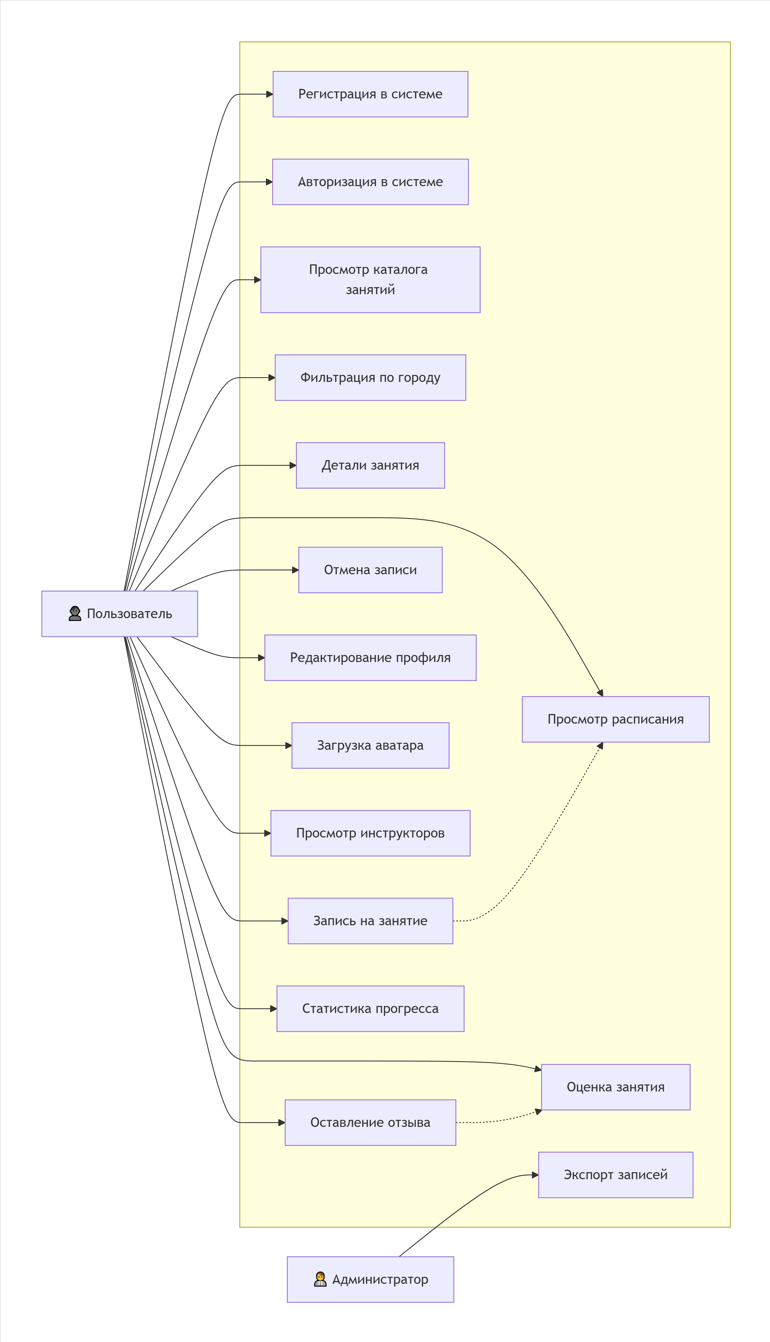
\includegraphics[width=0.8\textwidth]{images/use-case.png}
	\caption{Диаграмма прецедентов}
	\label{fig:usecase}
\end{figure}

Далее приведены агрегированные перечни прецедентов для каждой роли; они детализируются в последующих подпунктах.

\subsubsection{Вариант использования «Регистрация пользователя»}

\textbf{Предусловие:} приложение открыто на экране авторизации, пользователь не авторизован.

\textbf{Постусловие:} создана новая учётная запись, пользователь авторизован и перенаправлен на главный экран.

\textbf{Основной сценарий:}
\begin{enumerate}
	\item Пользователь нажимает кнопку «Регистрация».
	\item Система отображает форму регистрации.
	\item Пользователь вводит имя, адрес электронной почты, пароль и уровень подготовки.
	\item Пользователь нажимает кнопку «Зарегистрироваться».
	\item Система проверяет, не зарегистрирован ли уже указанный email.
	\item Если email свободен, система сохраняет данные в SharedPreferences.
	\item Система автоматически выполняет вход и открывает главный экран.
\end{enumerate}

\textbf{Альтернативный сценарий A1 (email уже зарегистрирован):}
\begin{enumerate}
	\item Система обнаруживает, что указанный email уже существует.
	\item Система отображает сообщение «Пользователь с таким email уже существует».
	\item Регистрация не выполняется, форма остаётся открытой.
\end{enumerate}

\textbf{Альтернативный сценарий A2 (не заполнены обязательные поля):}
\begin{enumerate}
	\item Система обнаруживает, что не все обязательные поля заполнены.
	\item Система подсвечивает незаполненные поля и отображает сообщение «Заполните все поля».
	\item Регистрация не выполняется.
\end{enumerate}

\subsubsection{Вариант использования «Авторизация пользователя»}

\textbf{Предусловие:} приложение открыто на экране авторизации, пользователь зарегистрирован.

\textbf{Постусловие:} пользователь авторизован и перенаправлен на главный экран.

\textbf{Основной сценарий:}
\begin{enumerate}
	\item Пользователь вводит адрес электронной почты и пароль.
	\item Пользователь нажимает кнопку «Войти».
	\item Система проверяет соответствие данных в SharedPreferences.
	\item Данные верны, система открывает главный экран.
\end{enumerate}

\textbf{Альтернативный сценарий A1 (неверный email или пароль):}
\begin{enumerate}
	\item Система проверяет данные и обнаруживает несоответствие.
	\item Система отображает сообщение «Неверный email или пароль».
	\item Пользователь остаётся на экране авторизации.
\end{enumerate}

\subsubsection{Вариант использования «Просмотр каталога занятий»}

\textbf{Предусловие:} пользователь авторизован, открыт главный экран.

\textbf{Постусловие:} отображён список доступных занятий.

\textbf{Основной сценарий:}
\begin{enumerate}
	\item Пользователь нажимает на вкладку «Занятия».
	\item Система загружает список занятий из SharedPreferences.
	\item Система отображает карточки занятий на экране.
	\item Пользователь просматривает список, прокручивая его.
\end{enumerate}

\textbf{Альтернативный сценарий A1 (список занятий пуст):}
\begin{enumerate}
	\item Система обнаруживает, что список занятий пуст.
	\item Система отображает сообщение «Нет доступных занятий».
\end{enumerate}

\subsubsection{Вариант использования «Фильтрация занятий по городу»}

\textbf{Предусловие:} открыт каталог занятий, список загружен.

\textbf{Постусловие:} отображаются только занятия выбранного города.

\textbf{Основной сценарий:}
\begin{enumerate}
	\item Пользователь нажимает на выпадающий список выбора города.
	\item Пользователь выбирает город (Москва, Санкт-Петербург или Казань).
	\item Система применяет фильтр к текущему набору занятий.
	\item Система обновляет карточки занятий на экране.
\end{enumerate}

\subsubsection{Вариант использования «Просмотр детальной информации о занятии»}

\textbf{Предусловие:} занятие отображается в списке или на карте.

\textbf{Постусловие:} открыт экран с детальной информацией о занятии.

\textbf{Основной сценарий:}
\begin{enumerate}
	\item Пользователь нажимает на карточку занятия в списке.
	\item Система открывает экран деталей.
	\item Система отображает название, описание, инструктора, время, место, цену и количество свободных мест.
\end{enumerate}

\subsubsection{Вариант использования «Запись на занятие»}

\textbf{Предусловие:} открыт экран детальной информации о занятии, пользователь не записан на это занятие.

\textbf{Постусловие:} запись сохранена, пользователь получает уведомление.

\textbf{Основной сценарий:}
\begin{enumerate}
	\item Пользователь нажимает кнопку «Записаться».
	\item Система проверяет наличие свободных мест.
	\item Места есть, система сохраняет запись в SharedPreferences.
	\item Система отправляет уведомление о подтверждении записи.
	\item Количество свободных мест уменьшается на 1.
\end{enumerate}

\textbf{Альтернативный сценарий A1 (нет свободных мест):}
\begin{enumerate}
	\item Система обнаруживает, что свободных мест нет.
	\item Система отображает сообщение «Нет свободных мест».
	\item Кнопка «Записаться» становится неактивной.
\end{enumerate}

\textbf{Альтернативный сценарий A2 (пользователь уже записан):}
\begin{enumerate}
	\item Система проверяет, не записан ли уже пользователь.
	\item Пользователь уже записан, система отображает сообщение «Вы уже записаны на это занятие».
\end{enumerate}

\subsubsection{Вариант использования «Отмена записи»}

\textbf{Предусловие:} пользователь записан на занятие, занятие ещё не началось.

\textbf{Постусловие:} запись удалена, место освобождено.

\textbf{Основной сценарий:}
\begin{enumerate}
	\item Пользователь открывает раздел «Мои записи».
	\item Пользователь выбирает запись для отмены.
	\item Пользователь нажимает кнопку «Отменить запись».
	\item Система удаляет запись из SharedPreferences.
	\item Система отображает сообщение «Запись отменена».
\end{enumerate}

\subsubsection{Вариант использования «Просмотр расписания с календарём»}

\textbf{Предусловие:} открыт раздел «Расписание».

\textbf{Постусловие:} отображены занятия на выбранную дату.

\textbf{Основной сценарий:}
\begin{enumerate}
	\item Пользователь открывает раздел «Расписание».
	\item Система отображает календарь на текущий месяц.
	\item Пользователь выбирает дату в календаре.
	\item Система фильтрует занятия по выбранной дате.
	\item Система отображает список занятий на выбранную дату.
\end{enumerate}

\subsubsection{Вариант использования «Просмотр списка инструкторов»}

\textbf{Предусловие:} открыт раздел «Инструкторы».

\textbf{Постусловие:} отображён список инструкторов.

\textbf{Основной сценарий:}
\begin{enumerate}
	\item Пользователь открывает раздел «Инструкторы».
	\item Система загружает список инструкторов из SharedPreferences.
	\item Система отображает карточки инструкторов на экране.
	\item При необходимости пользователь может отфильтровать инструкторов по городу.
\end{enumerate}

\subsubsection{Вариант использования «Редактирование профиля»}

\textbf{Предусловие:} открыт раздел «Профиль».

\textbf{Постусловие:} данные профиля обновлены.

\textbf{Основной сценарий:}
\begin{enumerate}
	\item Пользователь нажимает кнопку «Редактировать профиль».
	\item Система отображает форму с текущими данными.
	\item Пользователь изменяет нужные поля (аватар, имя, email, город, уровень подготовки).
	\item Пользователь нажимает кнопку «Сохранить».
	\item Система обновляет данные в SharedPreferences.
	\item Система отображает обновлённый профиль.
\end{enumerate}

\subsubsection{Вариант использования «Просмотр прогресса в виде графиков»}

\textbf{Предусловие:} открыт раздел «Прогресс».

\textbf{Постусловие:} отображены графики прогресса.

\textbf{Основной сценарий:}
\begin{enumerate}
	\item Пользователь открывает раздел «Прогресс».
	\item Система загружает данные о посещениях из SharedPreferences.
	\item Система строит графики (количество занятий по месяцам).
	\item Пользователь просматривает статистику.
	\item При необходимости пользователь может переключить отображаемый период (неделя, месяц, год).
\end{enumerate}

\subsubsection{Вариант использования «Оставление отзыва и рейтинга»}

\textbf{Предусловие:} занятие завершено, пользователь не оставлял отзыв ранее.

\textbf{Постусловие:} отзыв сохранён.

\textbf{Основной сценарий:}
\begin{enumerate}
	\item Пользователь открывает завершённое занятие в разделе «Мои записи».
	\item Пользователь нажимает кнопку «Оставить отзыв».
	\item Система отображает форму отзыва.
	\item Пользователь выбирает рейтинг от 1 до 5 звёзд.
	\item Пользователь вводит текстовый комментарий (опционально).
	\item Пользователь нажимает кнопку «Сохранить».
	\item Система сохраняет отзыв в SharedPreferences.
	\item Система обновляет рейтинг инструктора.
\end{enumerate}

\subsubsection{Вариант использования «Просмотр списка активных записей»}

\textbf{Предусловие:} открыт раздел «Мои записи».

\textbf{Постусловие:} отображены активные записи пользователя.

\textbf{Основной сценарий:}
\begin{enumerate}
	\item Пользователь открывает раздел «Мои записи».
	\item Система загружает записи из SharedPreferences.
	\item Система отображает список с указанием даты, времени, типа занятия и статуса.
	\item За один час до начала занятия система автоматически отправляет пользователю напоминание о предстоящем занятии.
\end{enumerate}

\subsection{Требования к надёжности}

Приложение должно корректно обрабатывать следующие аварийные ситуации: отсутствие свободного места на устройстве, прерывание работы приложения вследствие входящего звонка или сворачивания, а также некорректный ввод данных пользователем, при котором система должна показывать сообщения об ошибке. Все операции записи и изменения данных должны быть атомарными, что исключает частичное сохранение информации. Приложение должно восстанавливать состояние после принудительного закрытия.

\subsection{Требования к информационной безопасности}

Пароли пользователей должны храниться в зашифрованном виде с использованием стандартных механизмов Android. Все данные пользователя хранятся локально на устройстве и не передаются сторонним сервисам. Доступ к данным профиля осуществляется только через приложение. При некорректном вводе данных система не должна раскрывать информацию о существовании других пользователей. Приложение должно запрашивать только необходимые разрешения (доступ к хранилищу для аватара, доступ к уведомлениям).

\subsection{Требования к программной и технической совместимости}

Система должна корректно функционировать на устройствах под управлением операционной системы Android версии не ниже 7.0 (API level 24). Для работы приложения необходим установленный пакет Google Play Services. Клиентская часть не требует наличия дополнительного программного обеспечения. Рекомендуемый объём оперативной памяти устройства составляет не менее 2 ГБ. Приложение должно поддерживать экраны с разрешением от 480x800 до 1440x2960 пикселей.

\subsection{Требования к оформлению документации}

Разработка программной документации производится согласно ГОСТ 19.102-77 «Единая система программной документации. Стадии разработки», ГОСТ 34.601-90 «Информационная технология. Комплекс стандартов на автоматизированные системы. Стадии создания», а также СТУ 04.02.030-2017 «Курсовые работы (проекты). Выпускные квалификационные работы. Общие требования к структуре и оформлению».
\section{Технический проект}

\subsection{Архитектура программной системы}

Разрабатываемая система представляет собой программно-информационную систему для организации и проведения занятий йогой — мобильное приложение «Йога-студия» для платформы Android. Приложение построено по принципу Single Activity с использованием фрагментов (Fragments). Архитектурная схема приложения представлена на рисунке \ref{fig:architecture}.

\begin{figure}[H]
	\centering
	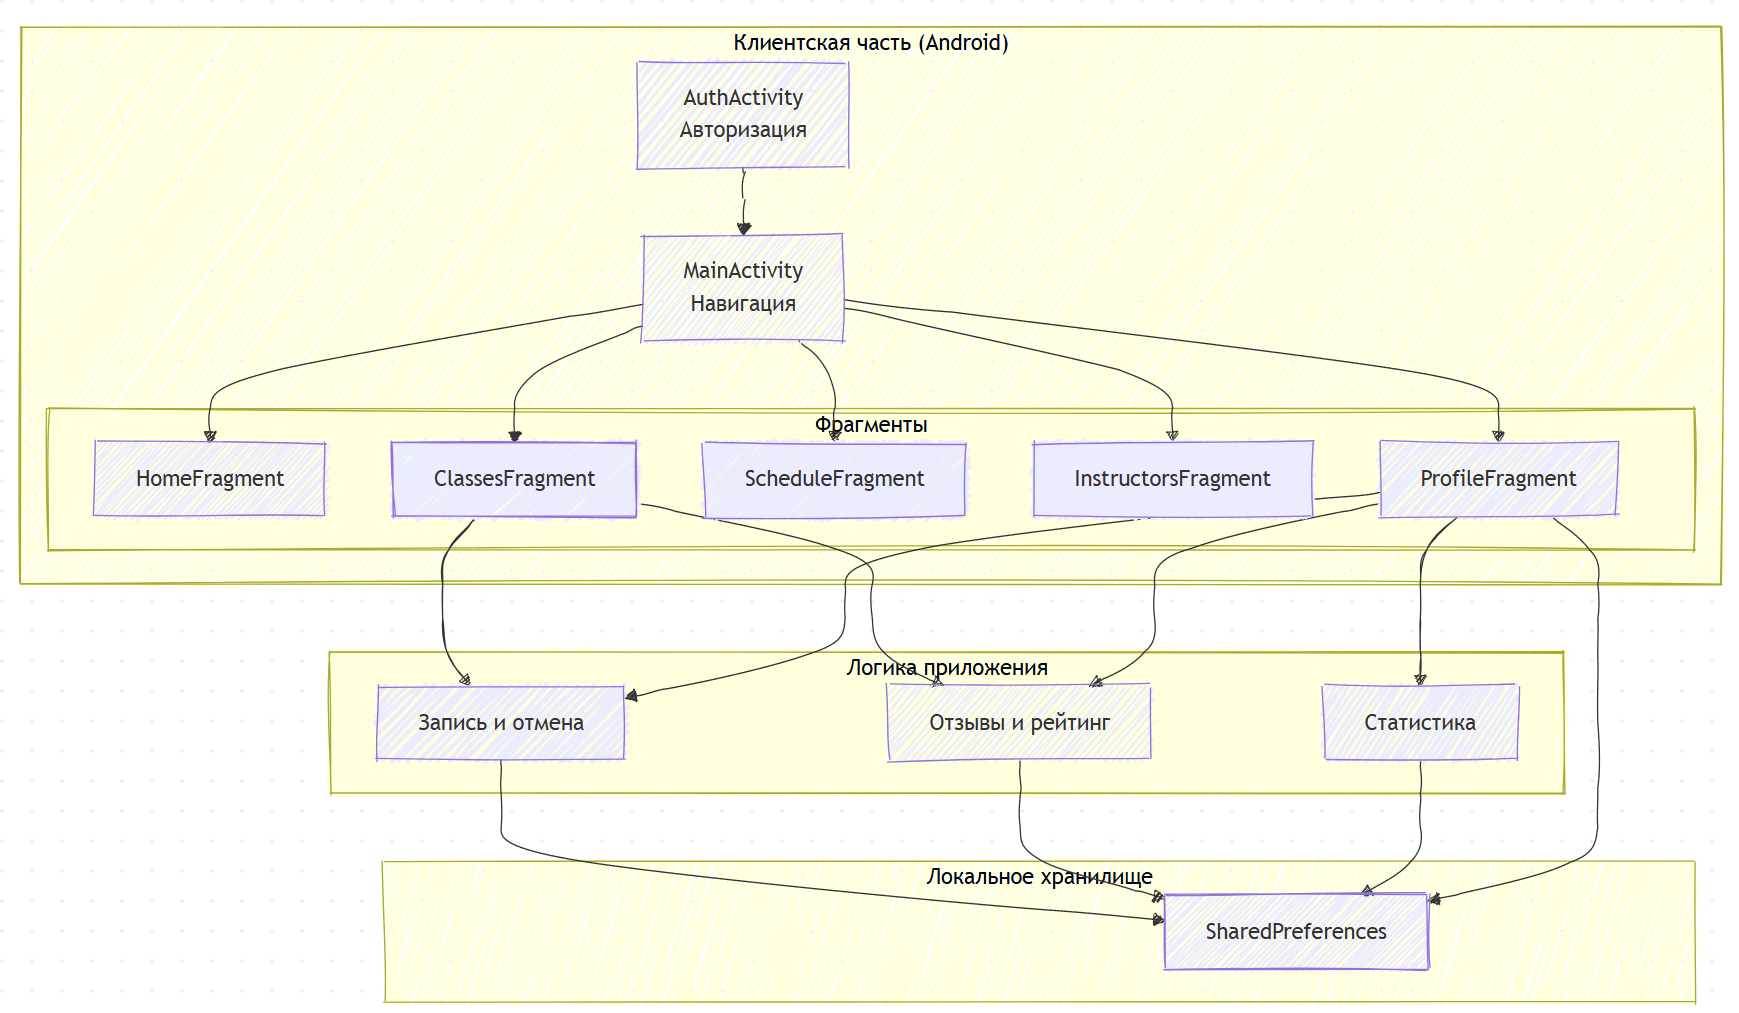
\includegraphics[width=0.9\textwidth]{images/architecture.png}
	\caption{Архитектурная схема приложения «Йога-студия»}
	\label{fig:architecture}
\end{figure}

Выбор такой архитектуры обоснован требованиями проекта: необходимо обеспечить одновременную работу пользовательской части (просмотр занятий, расписания, инструкторов) с единым хранилищем данных. Приложение централизует бизнес-логику и валидацию данных.

\subsection{Обоснование выбора технологий проектирования}

На сегодняшний день рынок мобильных разработок предлагает множество инструментов для создания приложений. Для достижения поставленной цели были выбраны следующие технологии.

\subsubsection{Kotlin как язык программирования}

Kotlin представляет собой современный статически типизированный язык программирования, работающий поверх Java Virtual Machine (JVM). Данный язык был официально рекомендован компанией Google для разработки под Android в 2017 году. Основными преимуществами Kotlin являются лаконичный и выразительный синтаксис, полная совместимость с Java, позволяющая использовать существующие Java-библиотеки, а также null-безопасность, которая существенно снижает количество ошибок во время выполнения. Кроме того, Kotlin поддерживает корутины для асинхронного программирования и имеет официальную поддержку в среде разработки Android Studio.

\subsubsection{Android SDK как фреймворк разработки}

Android Software Development Kit (SDK) представляет собой набор инструментов для разработки приложений под Android, включающий библиотеки, отладчик, эмулятор и документацию. В рамках данного проекта используются следующие основные компоненты Android SDK. Activity является основным компонентом для управления экранами. Fragment используется для создания модульных интерфейсов. RecyclerView применяется для отображения списков, таких как списки занятий и инструкторов. ViewPager2 используется для создания вкладок, в частности на экране авторизации.

\subsubsection{SharedPreferences как способ хранения данных}

Для хранения пользовательских данных, включая профиль, записи, отзывы и прогресс, используются SharedPreferences. Данный механизм представляет собой хранение пар «ключ-значение» локально на устройстве. Основными преимуществами SharedPreferences являются отсутствие необходимости подключения к интернету, простота реализации и сохранение данных даже после перезапуска приложения.

SharedPreferences поддерживает следующие типы данных: строки (String), целые числа (Int), логические значения (Boolean), числа с плавающей точкой (Float, Long), а также наборы строк (Set<String>). Для хранения сложных структур данных (например, списка занятий) используется преобразование в JSON-строку с помощью библиотеки Gson.

\subsubsection{Интеграция с MPAndroidChart для построения графиков}

Для визуализации прогресса пользователя в виде графиков используется библиотека MPAndroidChart. Данная библиотека предоставляет широкие возможности для построения различных типов диаграмм, включая линейные графики, гистограммы и круговые диаграммы. Библиотека имеет открытый исходный код и активно поддерживается сообществом разработчиков.

\subsection{Клиентская часть}

\subsubsection{Структура Activity и Fragments}

Приложение построено по принципу Single Activity с использованием фрагментов (Fragments). Основными компонентами приложения являются AuthActivity, представляющий собой экран авторизации и регистрации с вкладками, а также MainActivity, который является основным экраном с навигацией на основе BottomNavigationView.

Фрагмент HomeFragment отвечает за главный экран, отображающий приветствие, статистику и рекомендации. Фрагмент ClassesFragment реализует каталог занятий со списком и фильтрацией по городу. Фрагмент ScheduleFragment обеспечивает отображение расписания с календарём и списком занятий. Фрагмент InstructorsFragment отображает список инструкторов с фильтрацией по городу. Фрагмент ProfileFragment предоставляет профиль пользователя с аватаром и настройками.

Отдельные Activity используются для списка записей пользователя (MyBookingsActivity), экрана отзыва с рейтингом и комментарием (ReviewActivity), а также экрана статистики и графиков (ProgressActivity).

\subsubsection{Навигация и пользовательский интерфейс}

Навигация между разделами осуществляется с помощью BottomNavigationView, который позволяет переключаться между пятью основными экранами: главным, каталогом занятий, расписанием, инструкторами и профилем. При переходе между вкладками происходит замена одного фрагмента на другой в контейнере, расположенном в MainActivity. Пользовательский интерфейс выполнен с использованием компонентов Material Design, что обеспечивает современный внешний вид и интуитивно понятное взаимодействие.

\subsection{Диаграмма компонентов}

На рисунке \ref{fig:component} представлена диаграмма компонентов приложения, отражающая модульную структуру.

\begin{figure}[H]
	\centering
	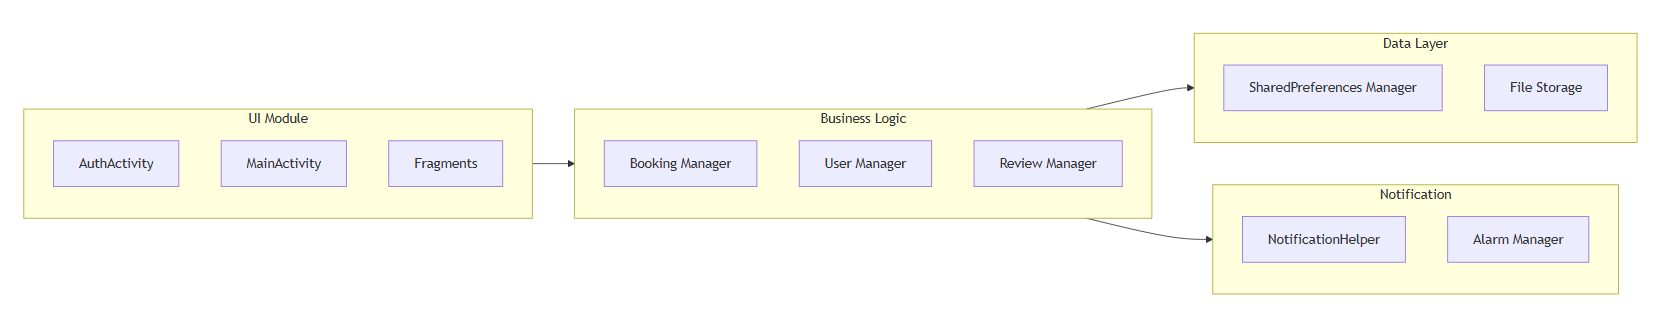
\includegraphics[width=0.9\textwidth]{images/component-diagram.png}
	\caption{Диаграмма компонентов}
	\label{fig:component}
\end{figure}

Приложение включает следующие компоненты: модуль авторизации (отвечает за вход и регистрацию пользователей), модуль навигации (обеспечивает переключение между вкладками), модуль занятий (управляет отображением каталога и деталей занятий), модуль расписания (предоставляет календарь и список занятий), модуль профиля (хранит и редактирует данные пользователя), модуль записей (управляет записью и отменой занятий), модуль отзывов (обрабатывает отзывы и рейтинг занятий), модуль статистики (отображает прогресс в виде графиков), модуль уведомлений (отправляет напоминания о занятиях).

\subsection{Диаграмма классов}

На рисунке \ref{fig:classdiagram} приведена диаграмма классов, отражающая объектную модель предметной области.

\begin{figure}[H]
	\centering
	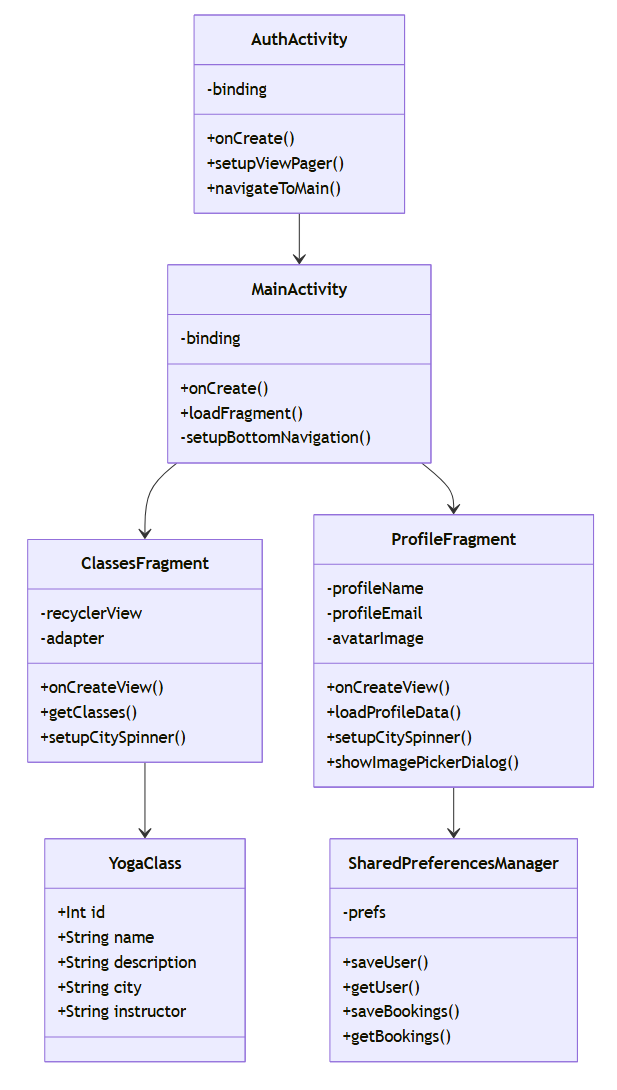
\includegraphics[width=0.7\textwidth]{images/class-diagram.png}
	\caption{Диаграмма классов}
	\label{fig:classdiagram}
\end{figure}

Основными классами приложения являются User (пользователь), Class (занятие), Instructor (инструктор), Booking (запись), Review (отзыв), Progress (прогресс). Класс User связан с Booking и Review. Класс Class связан с Instructor и Booking. Класс Progress связан с User.

\subsection{Диаграмма последовательности}

На рисунке \ref{fig:sequence} показана диаграмма последовательности для сценария «Запись на занятие», демонстрирующая взаимодействие компонентов.

\begin{figure}[H]
	\centering
	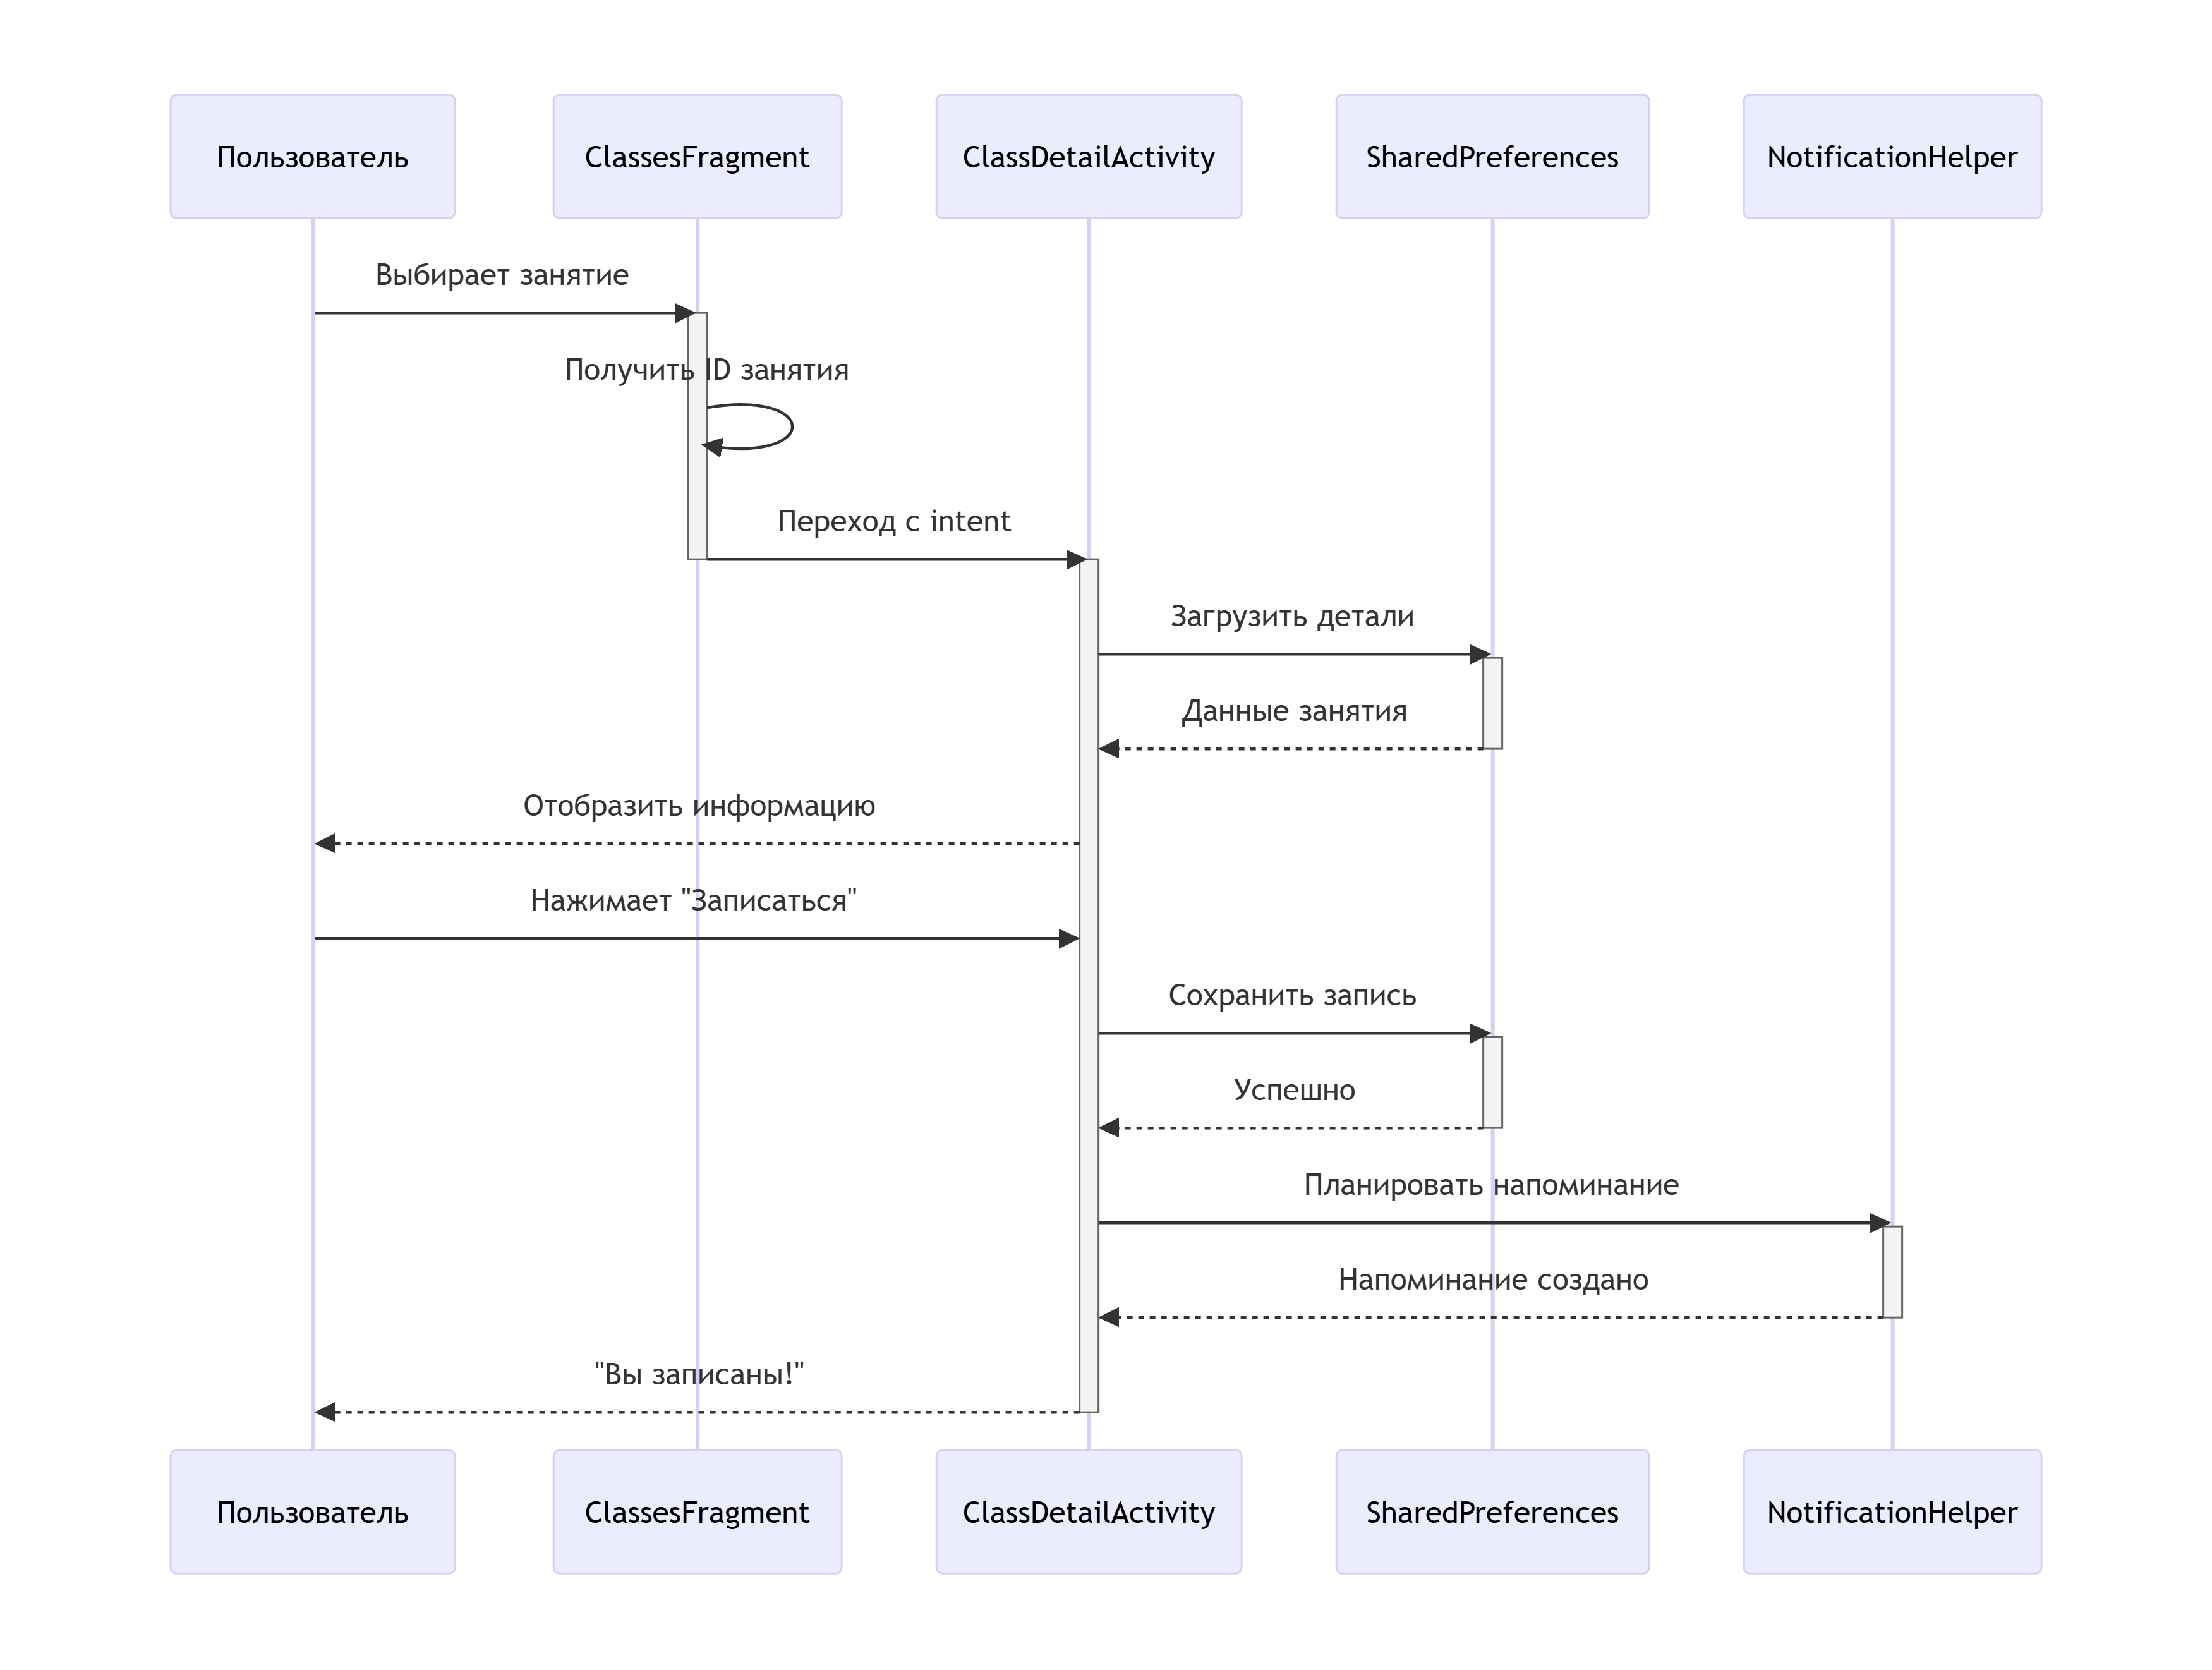
\includegraphics[width=0.9\textwidth]{images/sequence-diagram.png}
	\caption{Диаграмма последовательности (сценарий записи на занятие)}
	\label{fig:sequence}
\end{figure}

Пользователь выбирает занятие в ClassesFragment, система открывает экран деталей. При нажатии кнопки «Записаться» система проверяет наличие свободных мест в SharedPreferences. Если места есть, запись сохраняется, и отправляется уведомление через NotificationHelper.

\subsection{Диаграмма состояний}

На рисунке \ref{fig:state} представлена диаграмма состояний для жизненного цикла записи на занятие.

\begin{figure}[H]
	\centering
	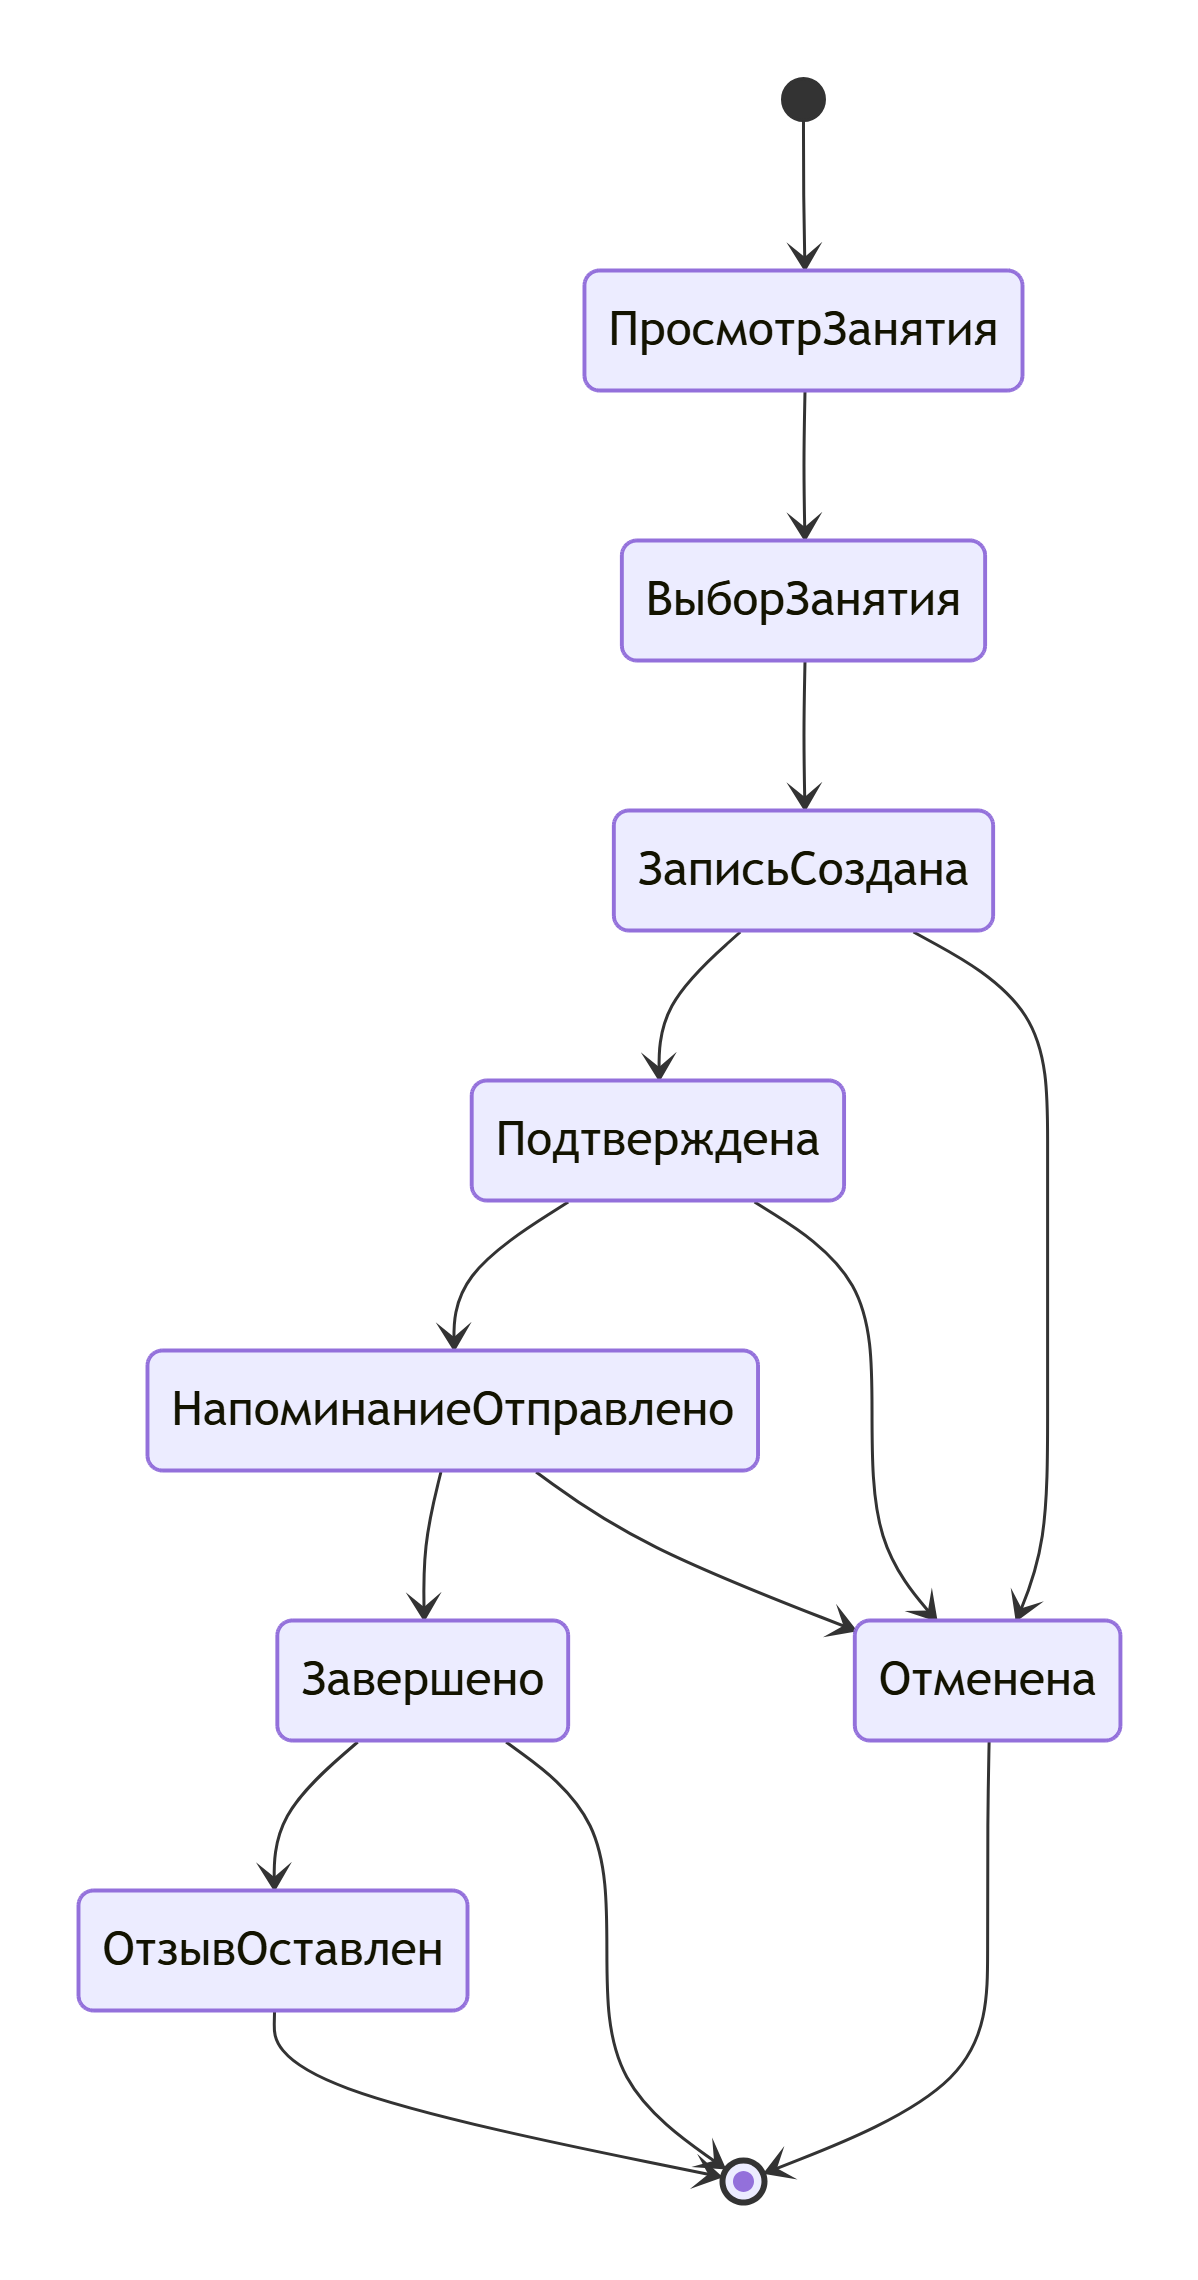
\includegraphics[width=0.7\textwidth]{images/state-diagram.png}
	\caption{Диаграмма состояний записи на занятие}
	\label{fig:state}
\end{figure}

Запись может находиться в следующих состояниях: просмотр занятия, выбор занятия, запись создана, подтверждена, напоминание отправлено, завершено, отменена, отзыв оставлен.

\subsection{Диаграмма взаимодействия фрагментов}

На рисунке \ref{fig:fragment} представлена диаграмма взаимодействия фрагментов в MainActivity, показывающая, как BottomNavigationView управляет загрузкой фрагментов.

\begin{figure}[H]
	\centering
	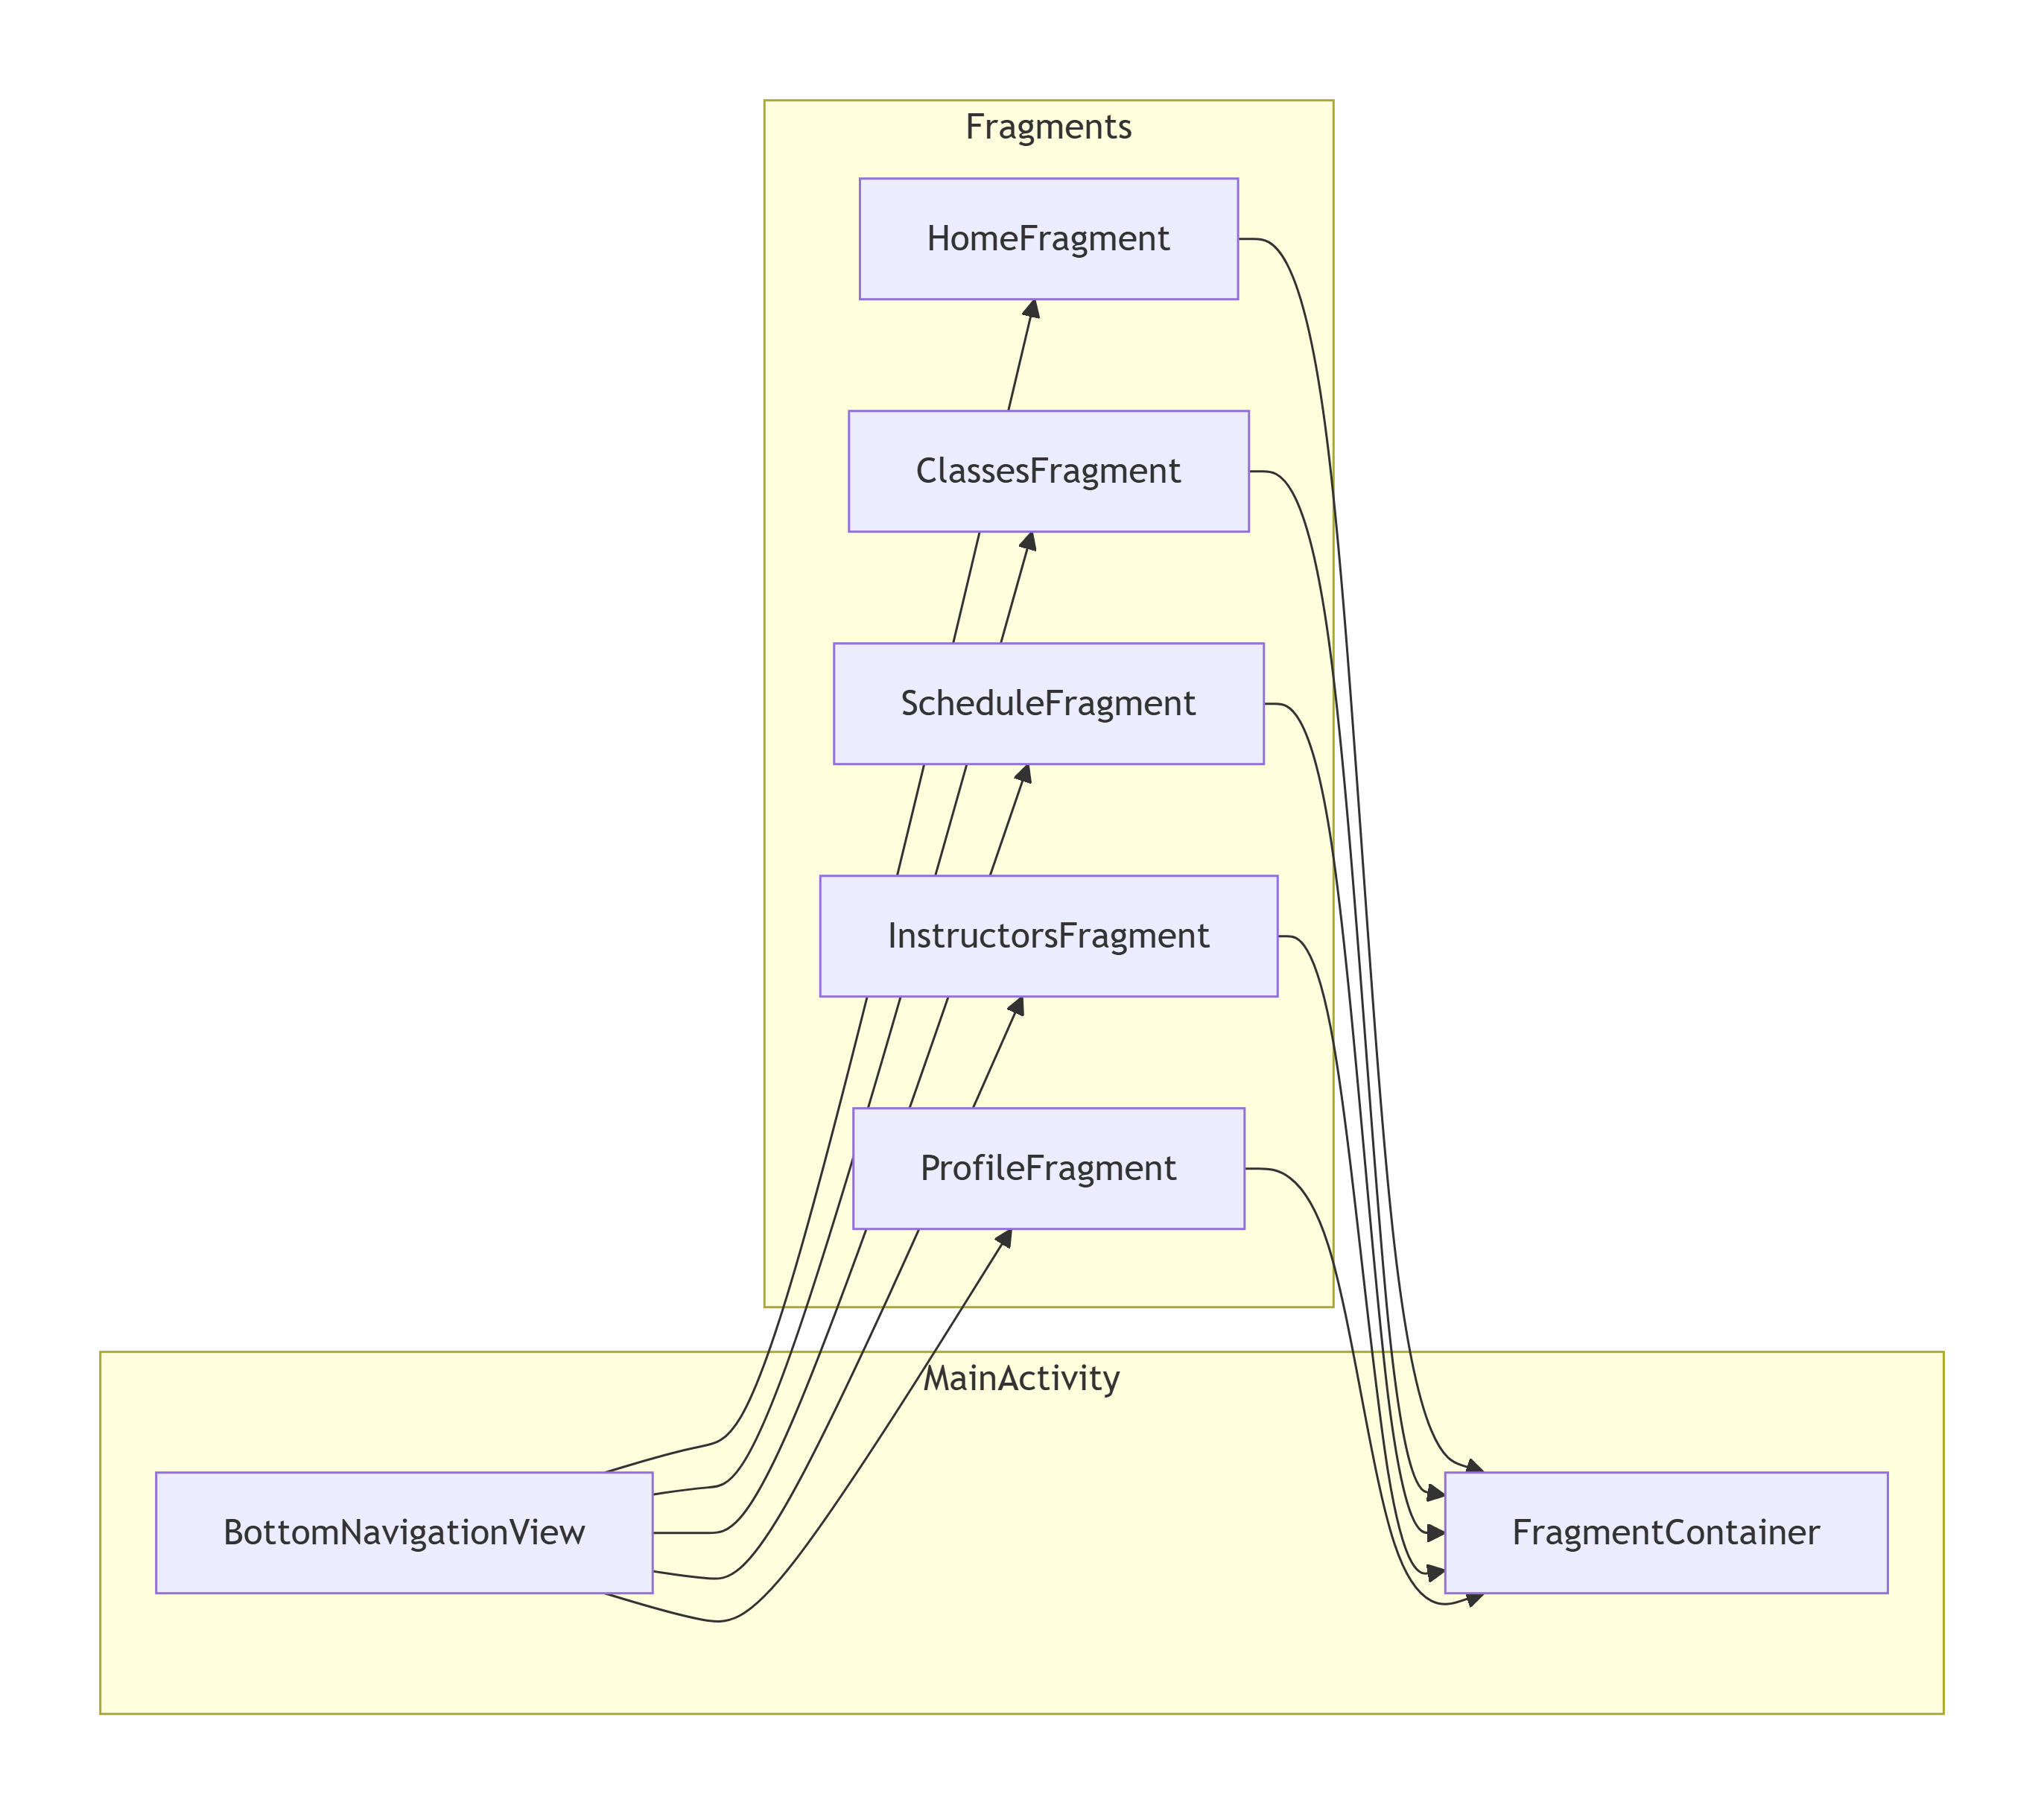
\includegraphics[width=0.9\textwidth]{images/fragment-interaction.png}
	\caption{Диаграмма взаимодействия фрагментов}
	\label{fig:fragment}
\end{figure}

BottomNavigationView обрабатывает выбор пункта меню и заменяет текущий фрагмент на соответствующий выбранному. Для управления фрагментами используется FragmentManager.

\subsection{Диаграмма пакетов}

На рисунке \ref{fig:package} представлена диаграмма пакетов, отражающая модульную структуру приложения на уровне пакетов.

\begin{figure}[H]
	\centering
	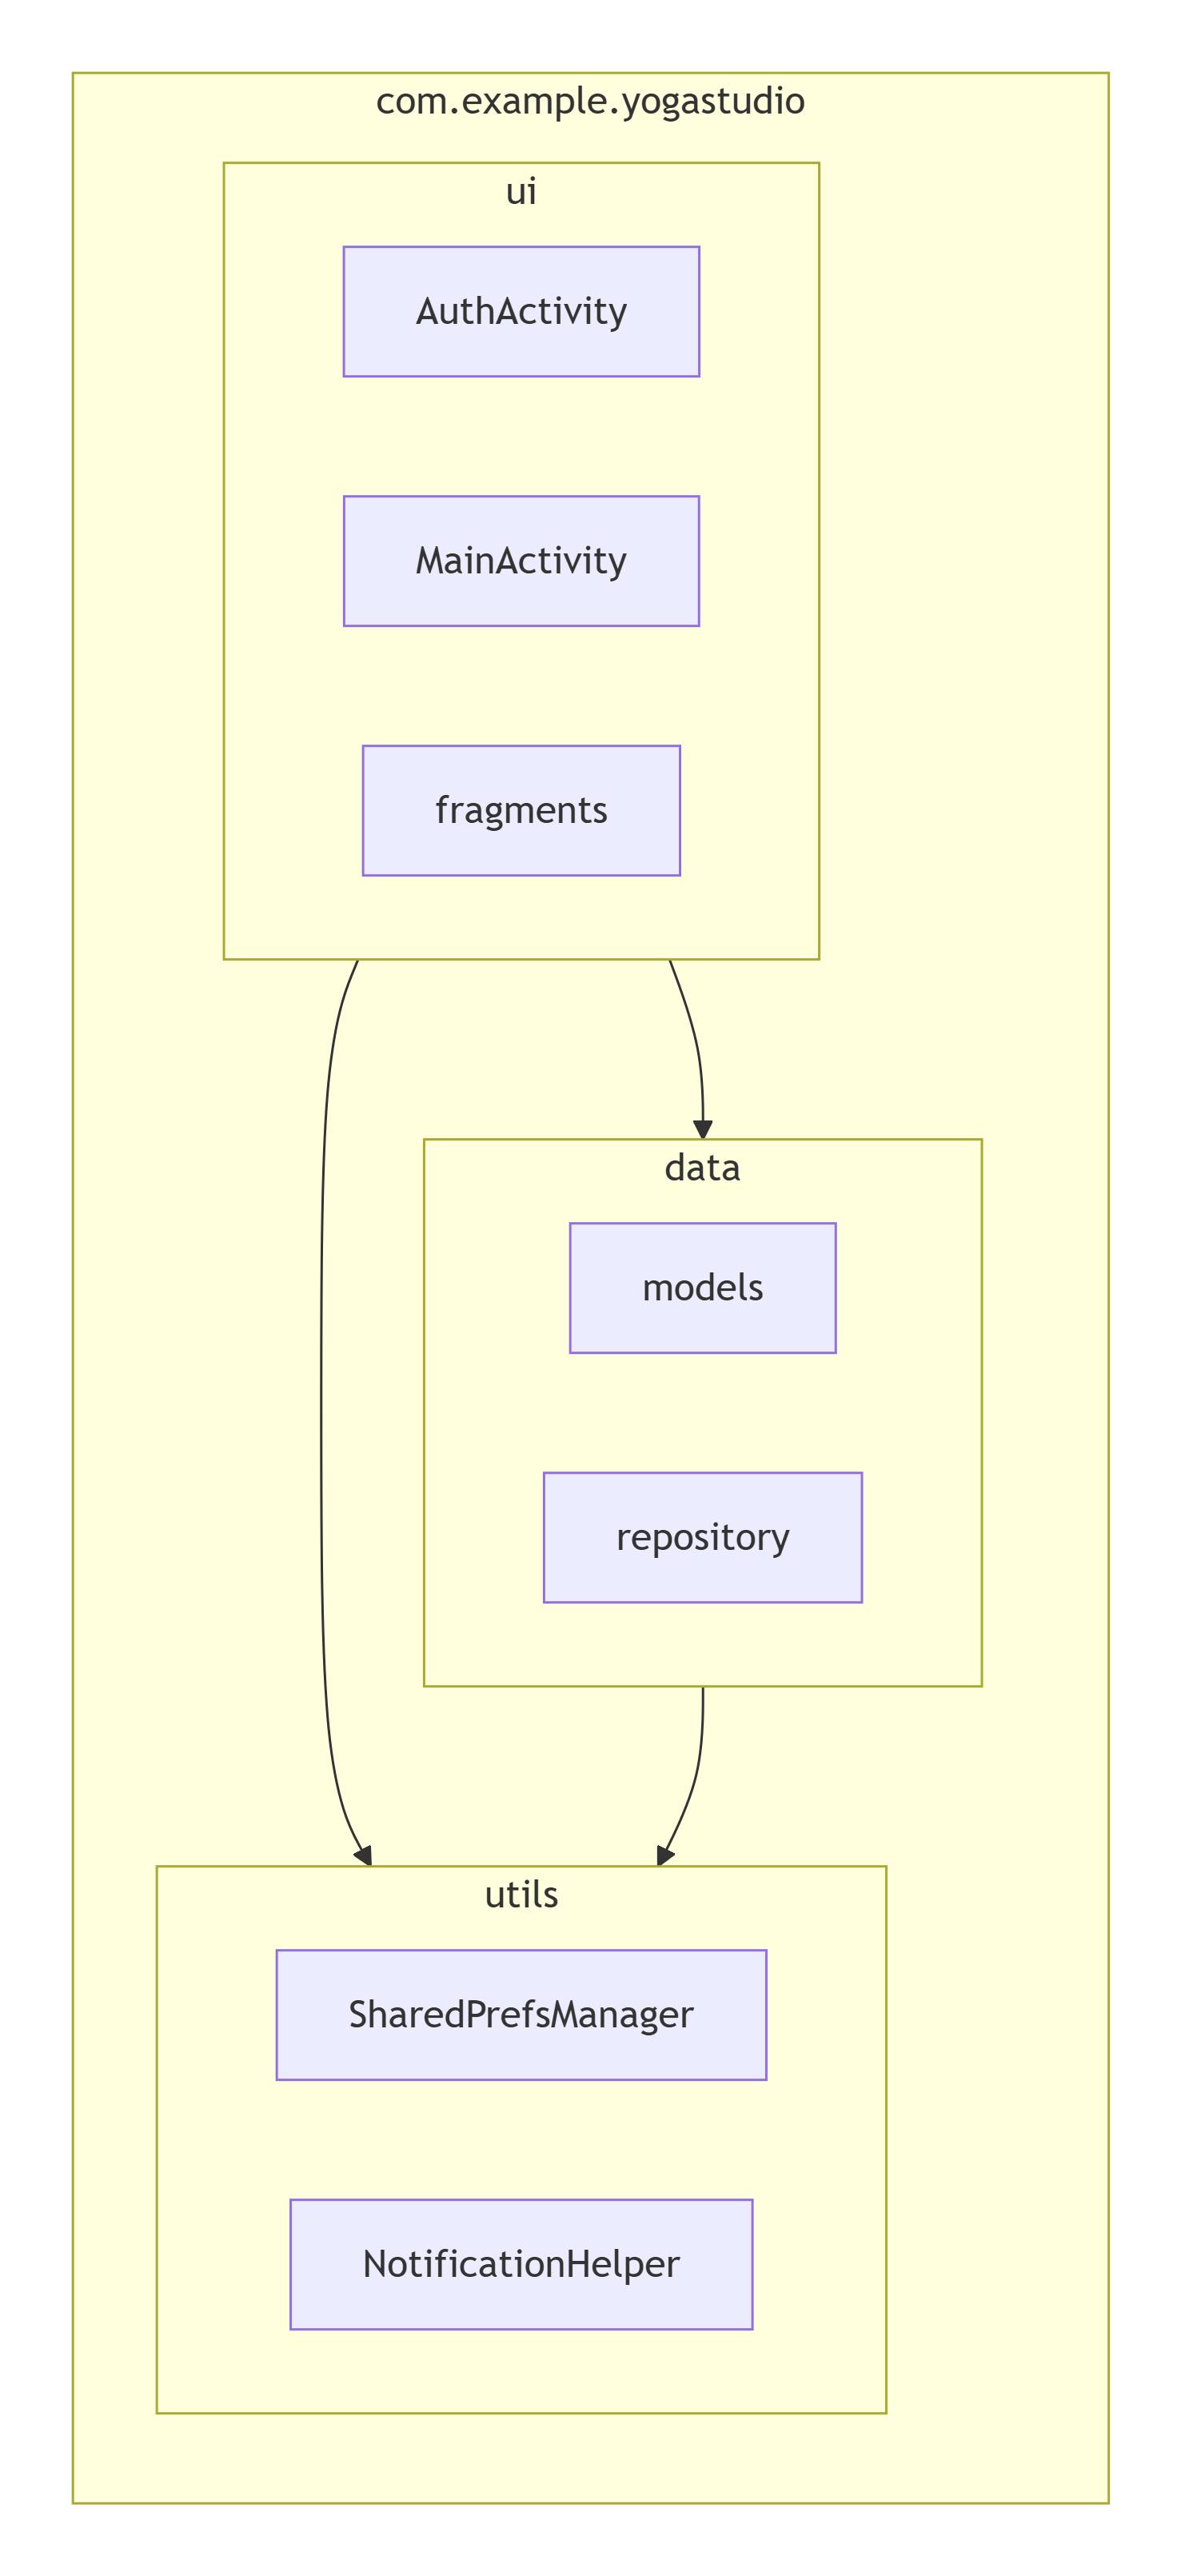
\includegraphics[width=0.7\textwidth]{images/package-diagram.png}
	\caption{Диаграмма пакетов}
	\label{fig:package}
\end{figure}

Приложение разделено на следующие пакеты: ui (пользовательский интерфейс), data (работа с данными), model (модели данных), utils (вспомогательные классы), notifications (уведомления).

\subsection{Диаграмма развертывания}

На рисунке \ref{fig:deployment} представлена диаграмма развертывания, показывающая физическую структуру системы: устройство пользователя, операционную систему Android и локальное хранилище.

\begin{figure}[H]
	\centering
	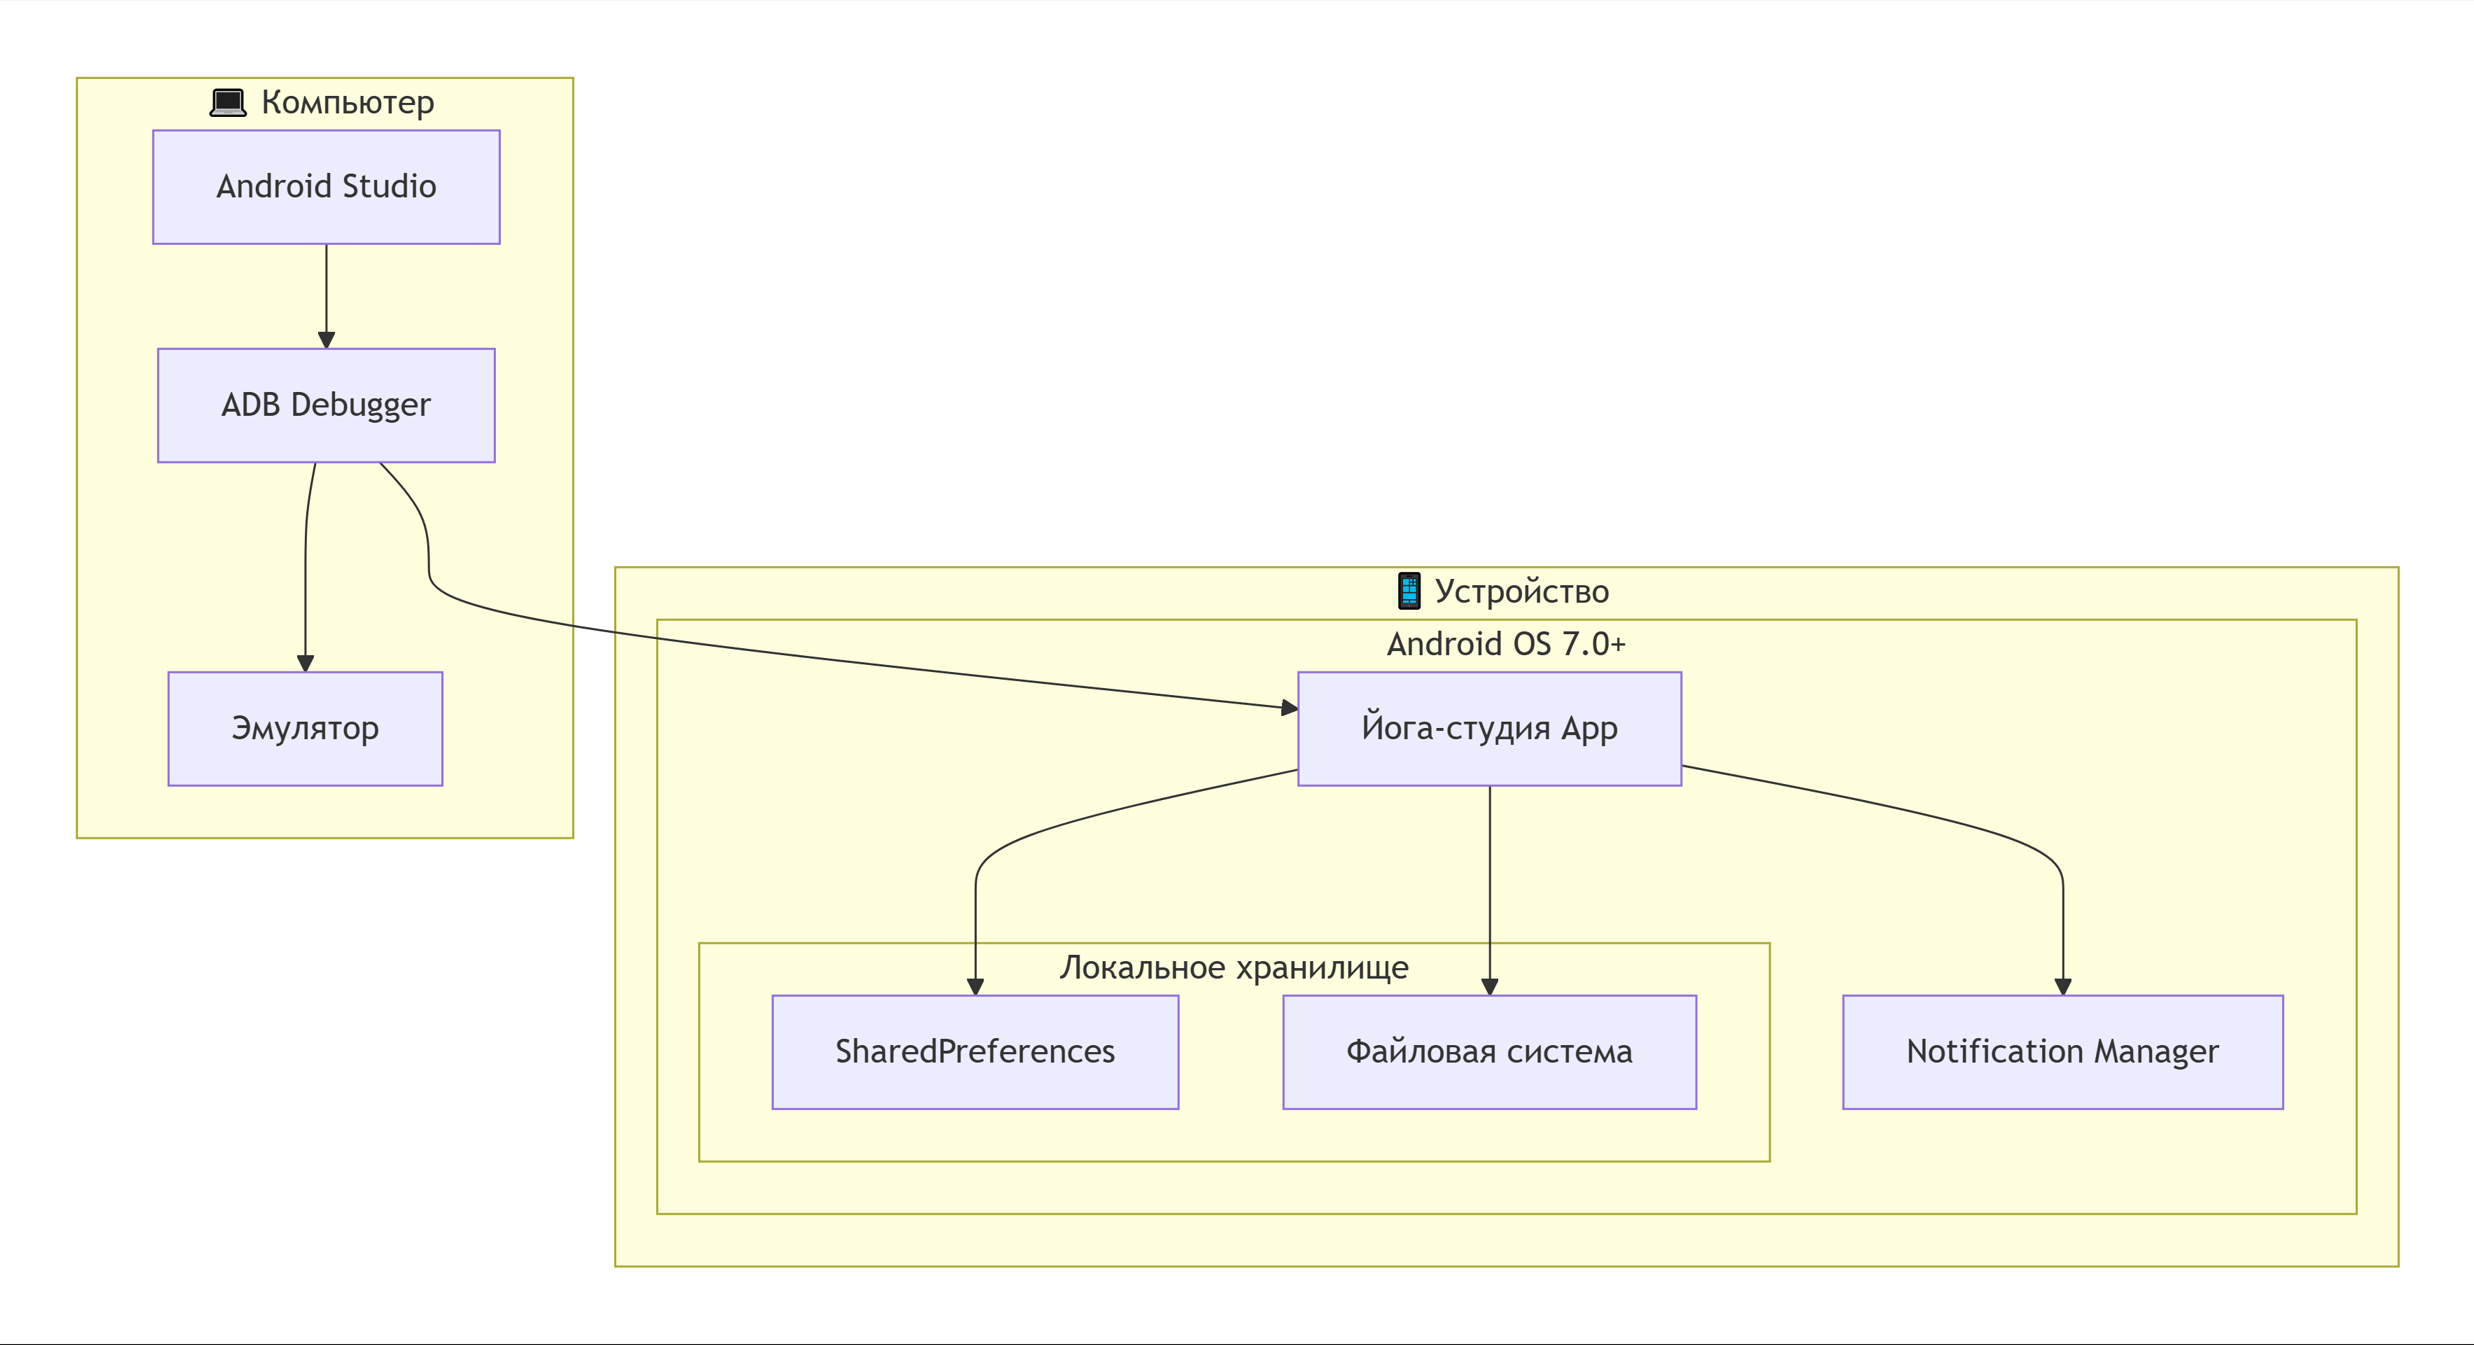
\includegraphics[width=0.9\textwidth]{images/deployment-diagram.png}
	\caption{Диаграмма развертывания}
	\label{fig:deployment}
\end{figure}

Приложение развертывается на физическом устройстве под управлением ОС Android. Для хранения данных используется внутренняя память устройства (SharedPreferences). Для разработки и отладки используется Android Studio с ADB Debugger и эмулятором.

\subsection{Проект базы данных (SharedPreferences)}

\subsubsection{Компоненты хранения данных}

Для хранения данных пользователя используются SharedPreferences, представляющие собой механизм хранения пар «ключ-значение» локально на устройстве. Данные сохраняются в XML-файле в защищённой области приложения. SharedPreferences поддерживает следующие типы данных: строки, целые числа, логические значения, числа с плавающей точкой и наборы строк (StringSet).

\subsubsection{ER-модель данных}

На рисунке \ref{fig:erdiagram} представлена ER-диаграмма сущностей, хранимых в SharedPreferences.

\begin{figure}[H]
	\centering
	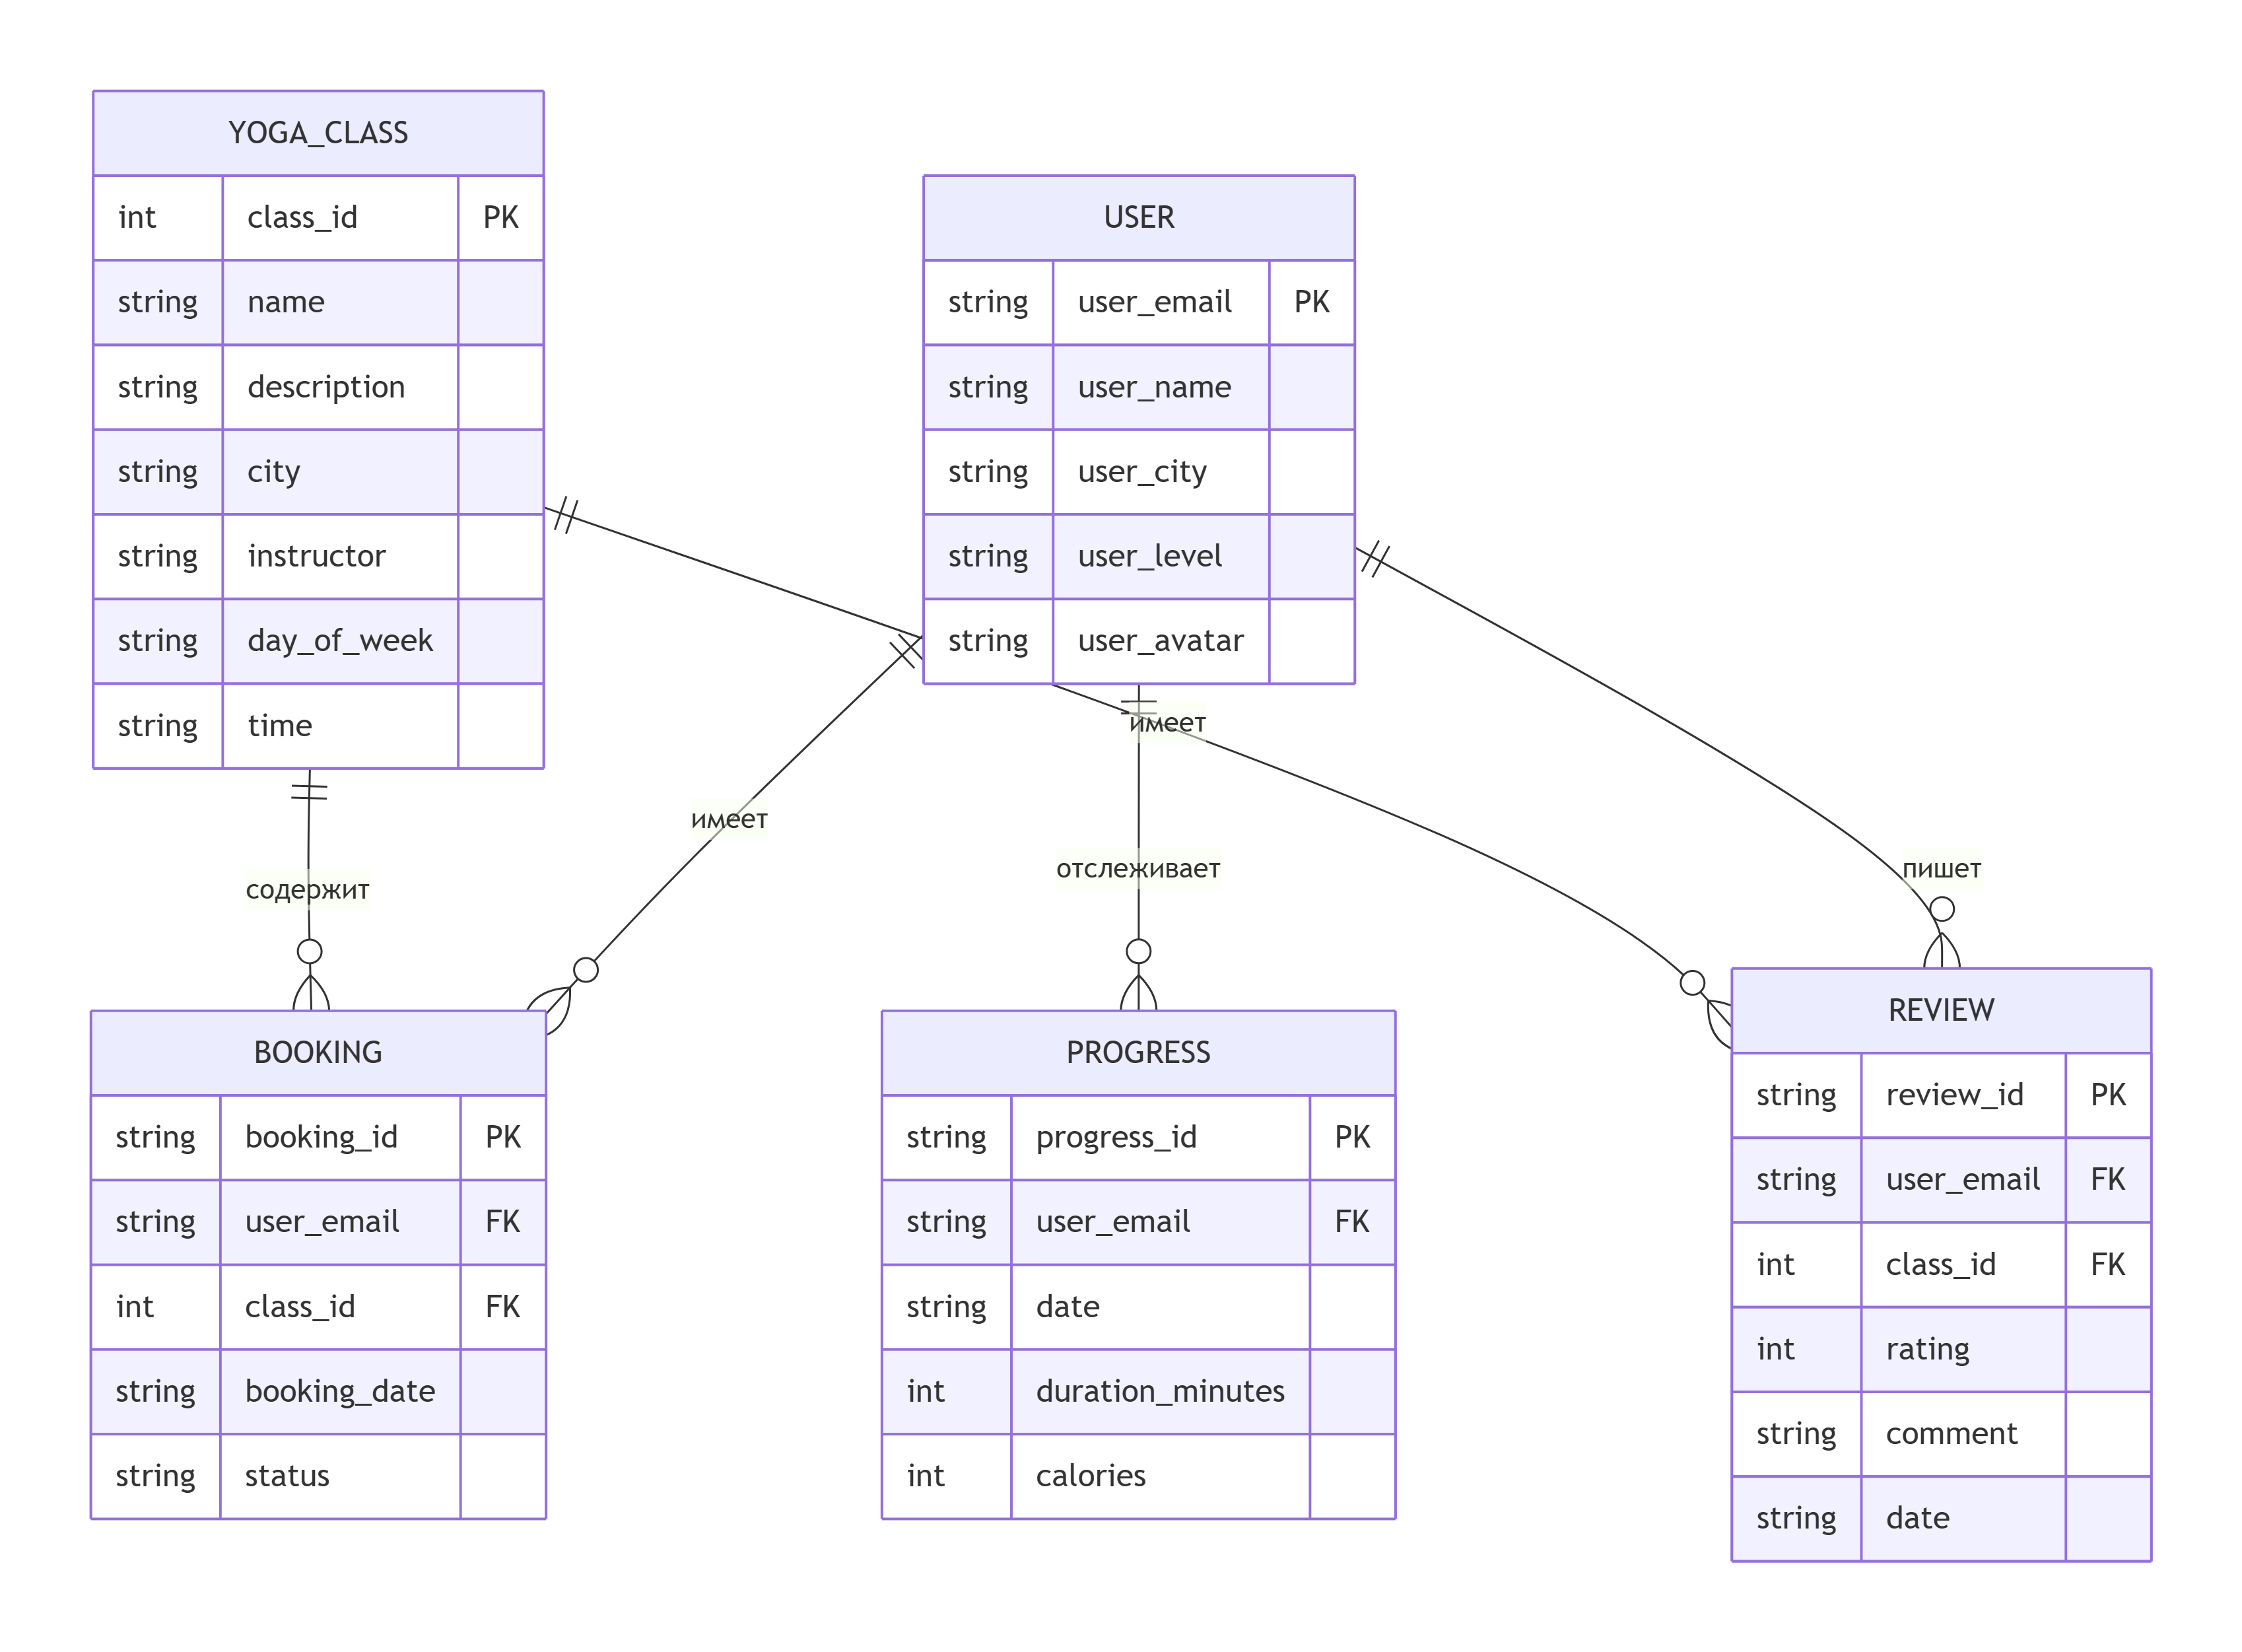
\includegraphics[width=0.9\textwidth]{images/er-diagram.png}
	\caption{ER-диаграмма сущностей}
	\label{fig:erdiagram}
\end{figure}

Ключевыми сущностями являются пользователь (USER), занятие (YOGA\_CLASS), запись (BOOKING), прогресс (PROGRESS) и отзыв (REVIEW). USER связан с BOOKING, PROGRESS и REVIEW. YOGA\_CLASS связан с BOOKING и REVIEW.

\subsubsection{Описание структуры ключей хранилища}

В таблице \ref{tab:sharedprefs} приведено описание основных ключей хранилища SharedPreferences.

\renewcommand{\arraystretch}{1.4}
\begin{table}[H]
	\centering
	\caption{Сущности хранилища SharedPreferences}
	\label{tab:sharedprefs}
	\normalsize
	\setlength{\tabcolsep}{6pt}
	\begin{tabular}{|m{3.3cm}|m{2.2cm}|m{3.5cm}|m{6.5cm}|}
		\hline
		\textbf{Ключ} & \textbf{Тип} & \textbf{Обязательное} & \textbf{Описание} \\
		\hline
		user\_name & String & да & Имя пользователя \\
		\hline
		user\_email & String & да & Адрес электронной почты пользователя \\
		\hline
		user\_avatar & String & нет & URI аватара пользователя \\
		\hline
		user\_city & String & да & Выбранный город (Москва, Санкт-Петербург, Казань) \\
		\hline
		user\_level & String & да & Уровень подготовки \\
		\hline
		user\_styles & StringSet & нет & Любимые стили йоги \\
		\hline
		user\_goals & StringSet & нет & Цели пользователя \\
		\hline
		bookings & StringSet & да & Записи на занятия \\
		\hline
		reviews\_list & String & нет & Список отзывов \\
		\hline
		progress\_list & String & нет & Данные о прогрессе \\
		\hline
		classes\_list & String & да & Список занятий (JSON) \\
		\hline
		instructors\_list & String & да & Список инструкторов (JSON) \\
		\hline
	\end{tabular}
\end{table}
\renewcommand{\arraystretch}{1}

\subsection{Надёжность, производительность и масштабирование}

\subsubsection{Надёжность операций сохранения данных}

Сценарий сохранения данных пользователя реализован с использованием атомарных операций SharedPreferences, что гарантирует целостность данных при любых обстоятельствах. При возникновении ошибки во время сохранения (например, при отсутствии свободного места) система возвращает соответствующее сообщение и не фиксирует частично сохранённые данные.

\subsubsection{Оптимизация загрузки списков}

Для отображения списков занятий, инструкторов и записей используется компонент RecyclerView, который обеспечивает эффективное использование памяти при прокрутке больших объёмов данных. Изображения аватаров пользователей загружаются асинхронно с помощью библиотеки CircleImageView, что предотвращает зависание интерфейса.

\subsubsection{Потенциал масштабирования}

Текущая архитектура допускает дальнейшее масштабирование приложения. При увеличении объёма данных возможен переход от локального хранения SharedPreferences к облачной базе данных (например, Firebase Firestore) без кардинальной перестройки архитектуры. Кроме того, архитектура позволяет добавлять новые типы занятий, категории и фильтры без изменения основных модулей.

\subsection{Информационная безопасность технического проекта}

\subsubsection{Профиль угроз}

Для проекта релевантны следующие угрозы. Несанкционированный доступ к данным пользователя возможен при компрометации устройства. Отправка некорректных или вредоносных данных в SharedPreferences может привести к нарушению целостности информации. Раскрытие внутренних ошибок приложения не должно содержать конфиденциальной информации.

\subsubsection{Меры защиты}

В техническом проекте применяются следующие меры защиты. Пароли пользователей сохраняются в зашифрованном виде с использованием алгоритмов шифрования Android. Все операции с SharedPreferences выполняются в изолированном контейнере приложения. Валидация входных данных выполняется как на уровне пользовательского интерфейса, так и на уровне логики сохранения. Обработка ошибок реализована без вывода стектрейсов и внутренней информации приложения пользователю.

\subsection{Эксплуатация и развёртывание}

\subsubsection{Локальное развёртывание}

Для установки приложения на устройство пользователя необходимо скопировать APK-файл на устройство и разрешить установку из неизвестных источников. Приложение не требует дополнительной настройки после установки. Все данные сохраняются локально и доступны сразу после первого запуска.

\subsubsection{Конфигурация технических средств}

Для работы приложения требуется устройство под управлением операционной системы Android версии не ниже 7.0 (API level 24). Рекомендуемый объём оперативной памяти составляет не менее 2 ГБ. Свободное место на диске для установки приложения должно составлять не менее 50 МБ.

\subsubsection{Требования к устройству}

Минимальные технические требования к устройству включают процессор с частотой не менее 1,2 ГГц, 2 ГБ оперативной памяти и 50 МБ свободного дискового пространства. Устройство должно поддерживать работу с сенсорным экраном и иметь разрешение экрана не менее 480x800 пикселей.

\subsection{Верификация технического проекта}

\subsubsection{Функциональная верификация}

Функциональная верификация должна покрывать следующие сценарии. Проверка авторизации и регистрации пользователей с корректными и некорректными данными. Проверка фильтрации занятий по городу. Проверка записи на занятие и отмены записи. Проверка редактирования профиля пользователя. Проверка отображения графиков прогресса. Проверка оставления отзывов и рейтинга. Проверка получения уведомлений и напоминаний.

\subsubsection{Техническая верификация}

Техническая верификация должна включать проверку целостности данных после операций сохранения, проверку корректности работы приложения при отсутствии свободного места на устройстве, проверку работы приложения при сворачивании и восстановлении, а также проверку производительности при увеличении объёма данных.

\subsection{Выводы по разделу}

В данном разделе представлены архитектура и компоненты разрабатываемого мобильного приложения. Обоснован выбор технологий, включая язык Kotlin, Android SDK и SharedPreferences. Разработаны и представлены диаграммы, выполненные на языке UML: архитектурная схема, диаграмма компонентов, диаграмма классов, диаграмма последовательности, диаграмма деятельности, диаграмма состояний, диаграмма взаимодействия фрагментов, диаграмма пакетов, диаграмма развертывания, а также ER-диаграмма. Описаны основные сущности, хранимые в SharedPreferences. Разработанная архитектура обеспечивает модульность, удобство поддержки и масштабирования приложения.
\ifПрактика{}\else{
   \section{Рабочий проект}

\subsection{Реализация модуля авторизации и регистрации}

Модуль авторизации и регистрации реализован с использованием SharedPreferences для хранения данных пользователя. При регистрации система проверяет, не зарегистрирован ли уже указанный адрес электронной почты. Если пользователь с таким email не найден, данные сохраняются, и выполняется автоматический вход. При авторизации система сверяет введённые данные с сохранёнными.

На рисунке \ref{fig:auth} представлен экран авторизации и регистрации.

\begin{figure}[H]
	\centering
	
\includegraphics[width=0.4\textwidth]{images/auth.png}
	\caption{Экран авторизации}
	\label{fig:auth}
\end{figure}

\vspace{0.5cm}

\subsection{Реализация каталога занятий}

Каталог занятий реализован с использованием RecyclerView. Данные о занятиях хранятся в SharedPreferences в виде JSON-строк. При загрузке каталога система парсит данные и отображает карточки занятий. Фильтрация по городу реализована на клиентской стороне без дополнительных запросов к хранилищу.

На рисунке \ref{fig:classes} представлен экран каталога занятий.

\begin{figure}[H]
	\centering
	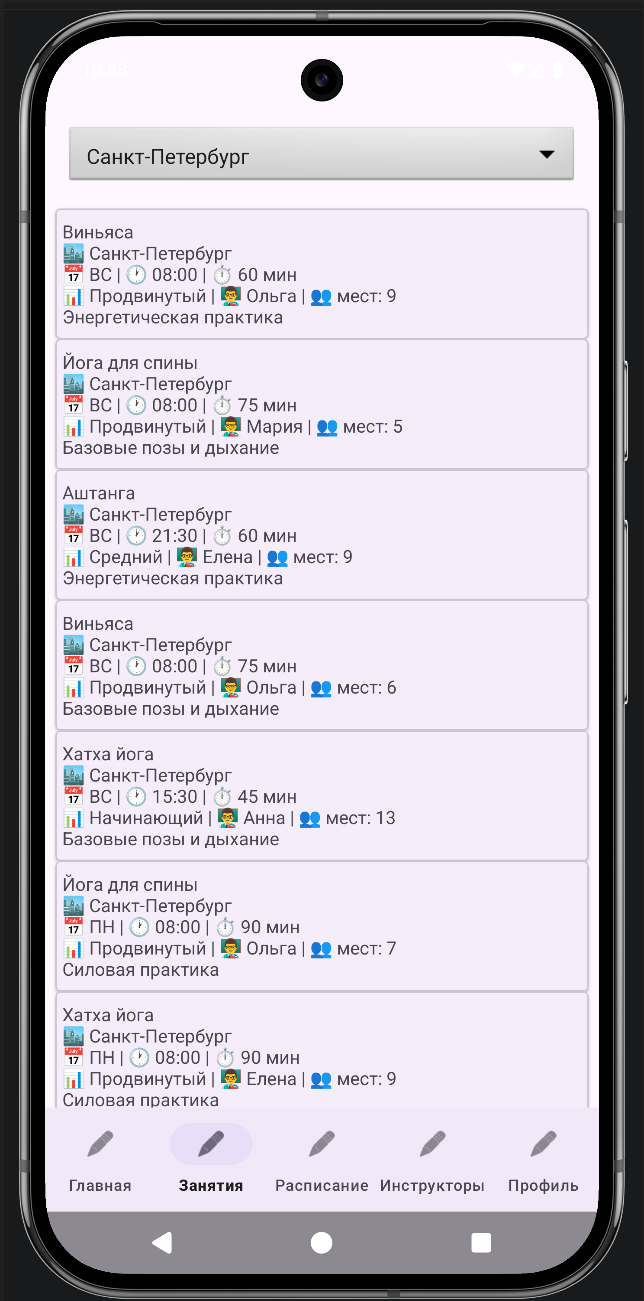
\includegraphics[width=0.4\textwidth]{images/classes.png}
	\caption{Каталог занятий}
	\label{fig:classes}
\end{figure}

\vspace{0.5cm}

\subsection{Реализация записи на занятие}

Запись на занятие реализована с проверкой наличия свободных мест. При успешной записи данные сохраняются в SharedPreferences, после чего система отправляет уведомление о подтверждении. Отмена записи удаляет соответствующий идентификатор из хранилища.

На рисунке \ref{fig:class_detail} представлен экран детальной информации о занятии с возможностью записи.

\begin{figure}[H]
	\centering
	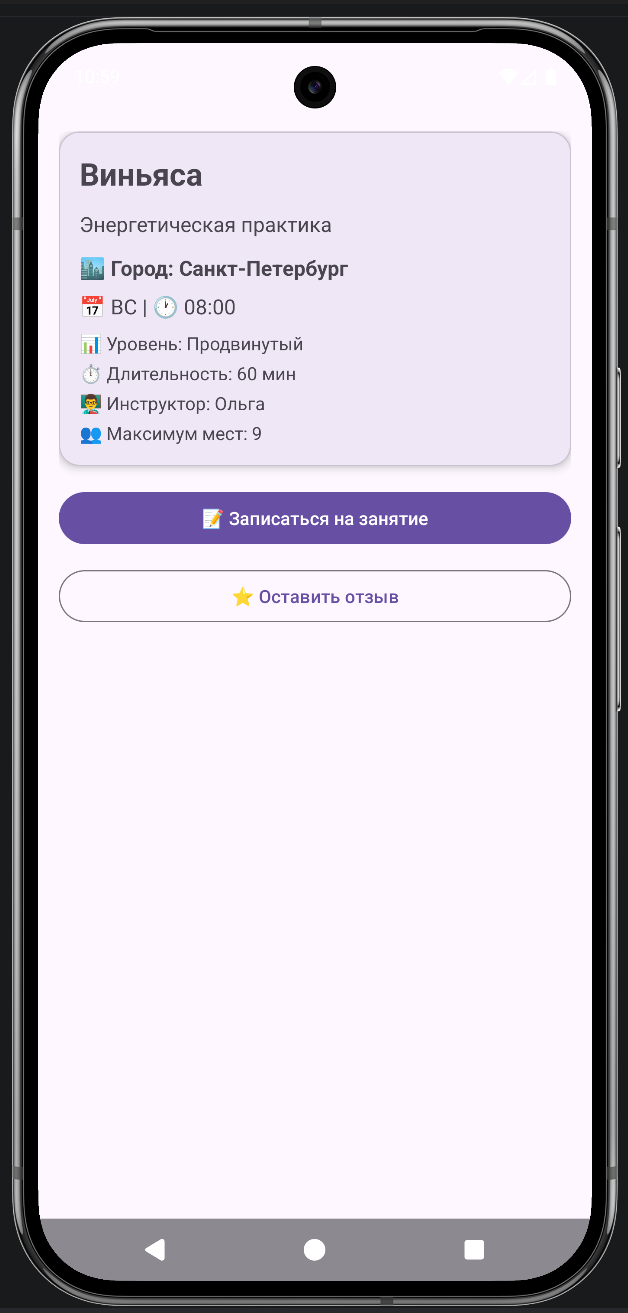
\includegraphics[width=0.4\textwidth]{images/class_detail.png}
	\caption{Детальная информация о занятии}
	\label{fig:class_detail}
\end{figure}

\vspace{0.5cm}

\subsection{Реализация расписания с календарём}

Расписание реализовано с использованием компонента CalendarView. При выборе даты система фильтрует занятия по выбранному дню и отображает список доступных занятий.

На рисунке \ref{fig:schedule} представлен экран расписания с календарём.

\begin{figure}[H]
	\centering
	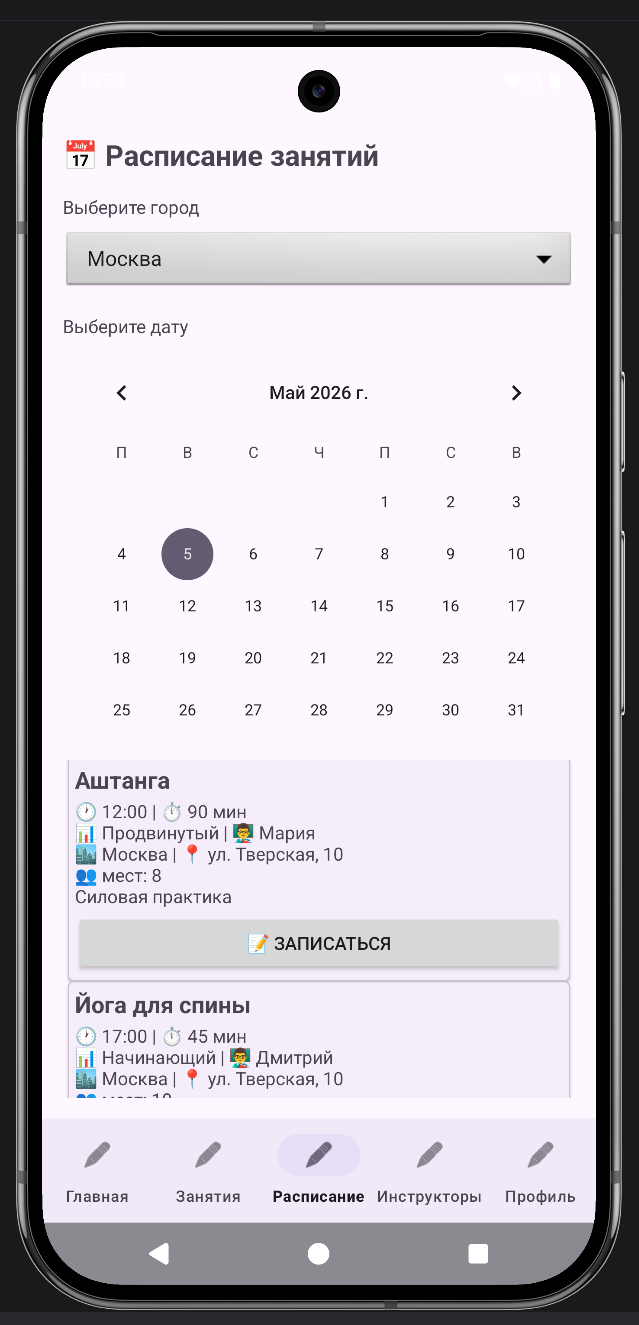
\includegraphics[width=0.4\textwidth]{images/schedule.png}
	\caption{Расписание с календарём}
	\label{fig:schedule}
\end{figure}

\vspace{0.5cm}

\subsection{Реализация профиля пользователя}

Профиль пользователя включает аватар, имя, адрес электронной почты, город и уровень подготовки. Для загрузки и отображения аватара используется библиотека CircleImageView. Все изменения сохраняются в SharedPreferences.

На рисунке \ref{fig:profile} представлен экран профиля пользователя.

\begin{figure}[H]
	\centering
	
\includegraphics[width=0.4\textwidth]{images/profile.png}
	\caption{Профиль пользователя}
	\label{fig:profile}
\end{figure}

\vspace{0.5cm}

\subsection{Реализация системы отзывов и рейтинга}

Отзывы и рейтинг хранятся в SharedPreferences. Пользователь может оставить отзыв только после посещения занятия. Рейтинг отображается в виде звёзд с использованием виджета RatingBar.

На рисунке \ref{fig:review} представлен экран оставления отзыва.

\begin{figure}[H]
	\centering
	
\includegraphics[width=0.4\textwidth]{images/review.png}
	\caption{Экран отзыва}
	\label{fig:review}
\end{figure}

\vspace{0.5cm}

\subsection{Реализация статистики и графиков}

Для построения графиков используется библиотека MPAndroidChart. Данные о посещениях загружаются из SharedPreferences, после чего система строит линейный график, отображающий количество занятий по месяцам.

На рисунке \ref{fig:progress} представлен экран статистики и графиков прогресса.

\begin{figure}[H]
	\centering
	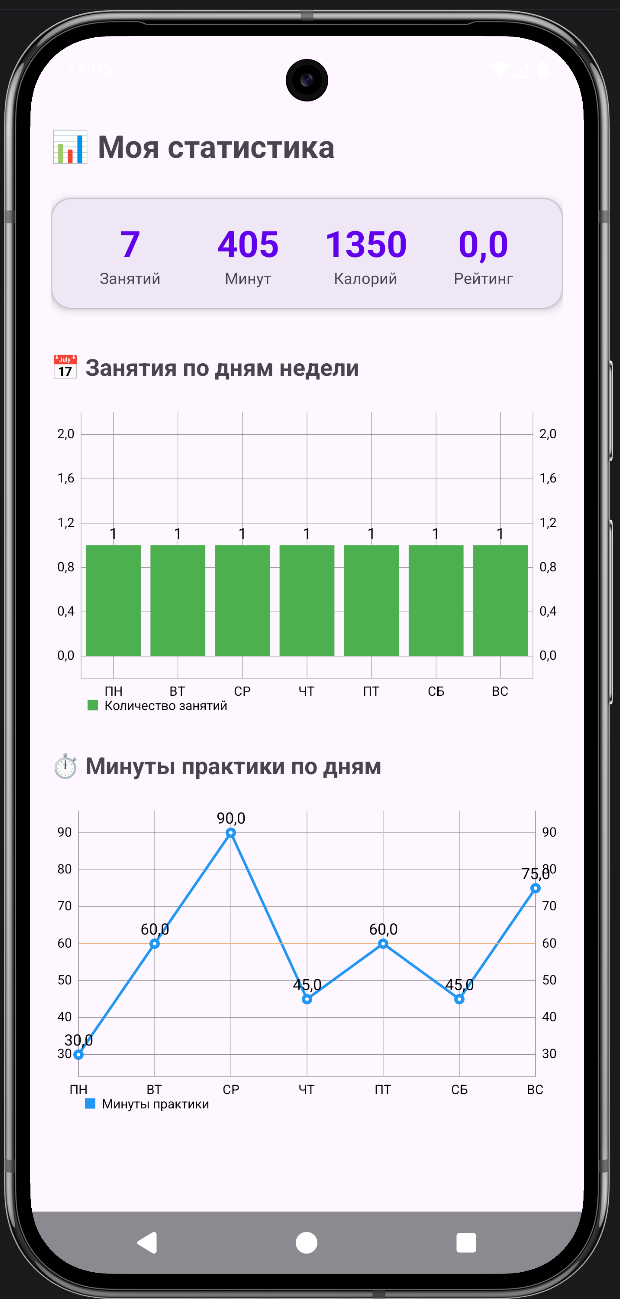
\includegraphics[width=0.4\textwidth]{images/progress.png}
	\caption{Статистика и графики прогресса}
	\label{fig:progress}
\end{figure}

\vspace{0.5cm}

\subsection{Реализация уведомлений и напоминаний}

Уведомления реализованы с использованием WorkManager для планирования напоминаний. За один час до начала занятия система отправляет push-уведомление пользователю. Уведомление о подтверждении записи отправляется сразу после успешного сохранения данных.

\subsection{Интерфейс приложения}

Пользовательский интерфейс реализован на языке разметки XML с использованием компонентов Material Design. Навигация между разделами осуществляется с помощью BottomNavigationView, который управляет загрузкой фрагментов. Все экраны приложения имеют единый стиль оформления.

На рисунке \ref{fig:home} представлен главный экран приложения.

\begin{figure}[H]
	\centering
	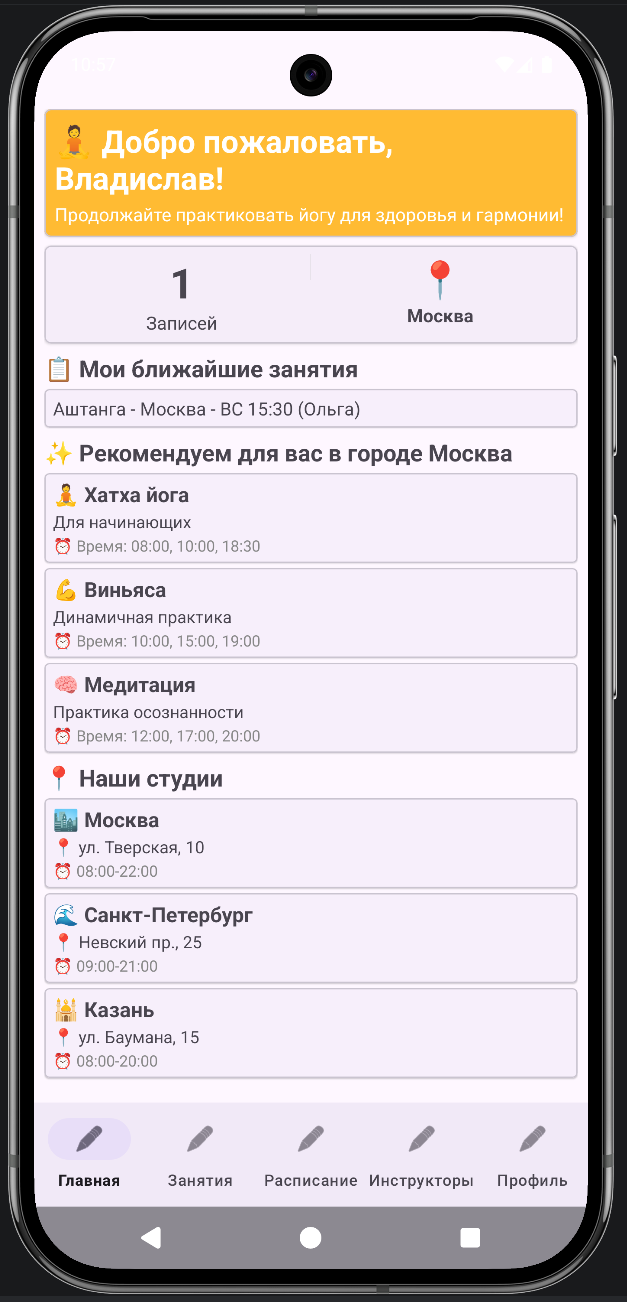
\includegraphics[width=0.4\textwidth]{images/home.png}
	\caption{Главный экран}
	\label{fig:home}
\end{figure}

\vspace{0.5cm}

На рисунке \ref{fig:instructors} представлен экран списка инструкторов.

\begin{figure}[H]
	\centering
	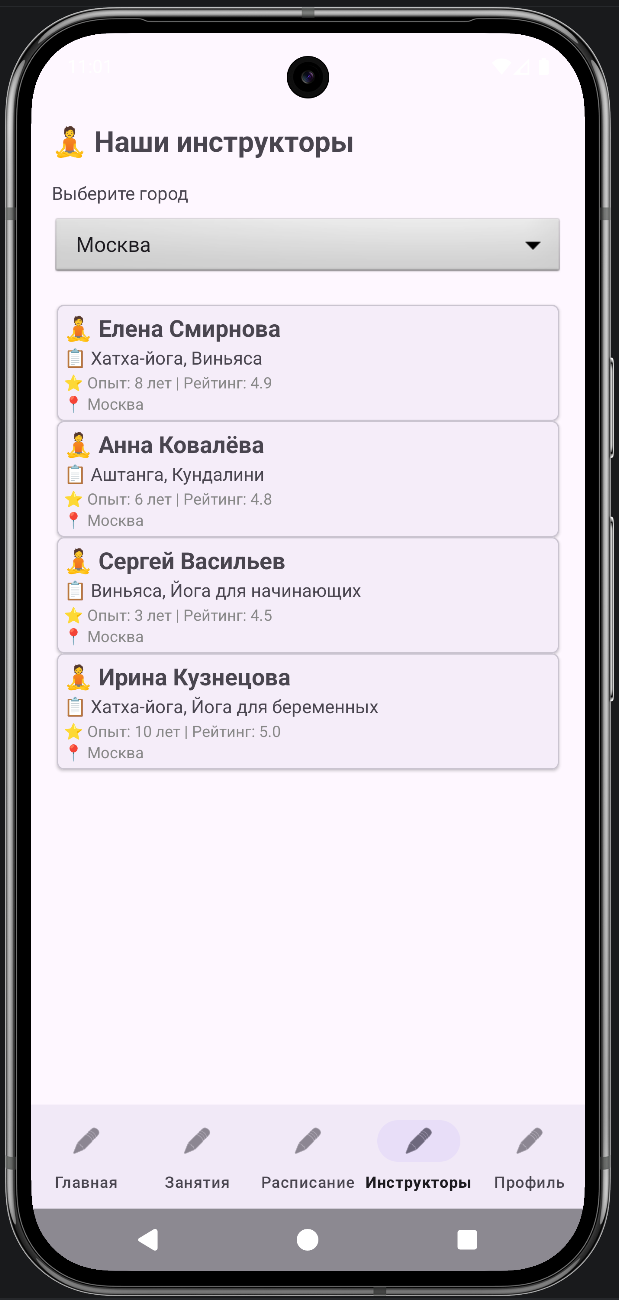
\includegraphics[width=0.4\textwidth]{images/instructors.png}
	\caption{Список инструкторов}
	\label{fig:instructors}
\end{figure}

\vspace{0.5cm}

На рисунке \ref{fig:bookings} представлен экран моих записей.

\begin{figure}[H]
	\centering
	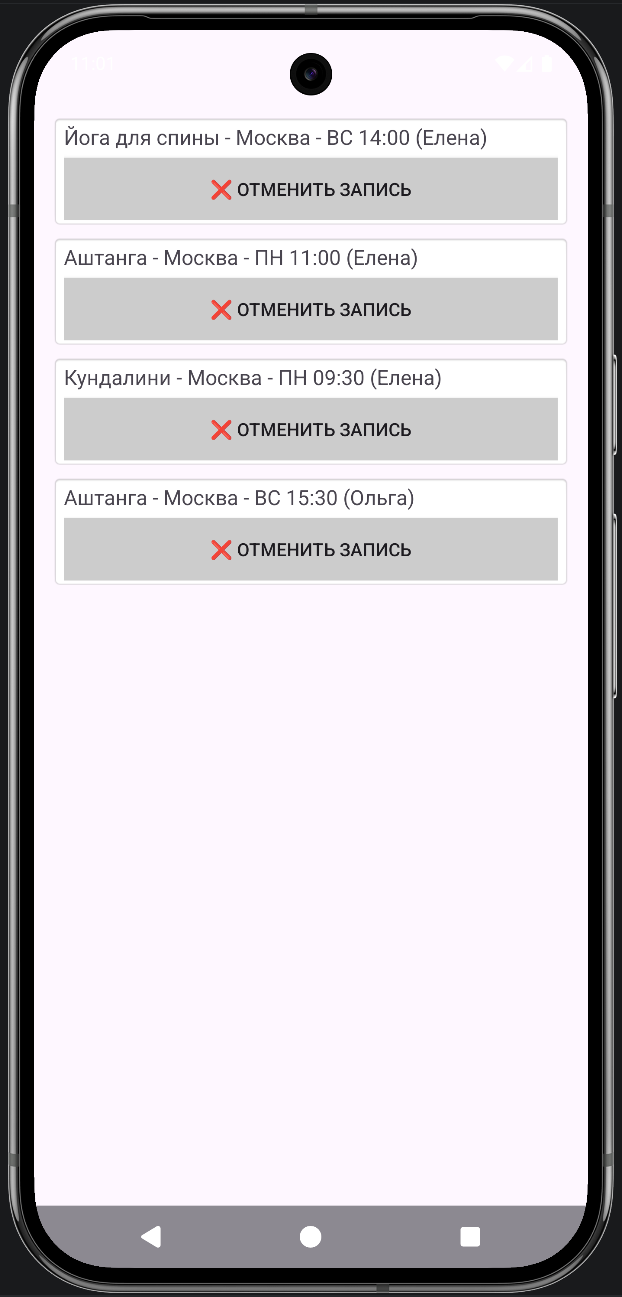
\includegraphics[width=0.4\textwidth]{images/bookings.png}
	\caption{Мои записи}
	\label{fig:bookings}
\end{figure}

\vspace{0.5cm}

\subsection{Тестирование приложения}

В ходе тестирования были проверены следующие сценарии: регистрация и авторизация пользователей, фильтрация занятий по городу, запись на занятие и отмена записи, редактирование профиля, построение графиков прогресса, оставление отзывов и рейтинга, получение уведомлений и напоминаний. Все сценарии отработали корректно.
   \section{Тестирование программной системы}

\subsection{Цели и задачи тестирования}

Целью тестирования является проверка соответствия разработанного приложения требованиям, сформулированным в техническом задании, а также выявление и устранение дефектов.

Основные задачи тестирования:
\begin{enumerate}
	\item проверка корректности реализации функциональных требований;
	\item проверка устойчивости приложения к некорректному вводу данных;
	\item проверка производительности приложения;
	\item проверка работы приложения в условиях ограниченных ресурсов;
	\item проверка совместимости с различными версиями Android.
\end{enumerate}

\subsection{План тестирования}

Тестирование проводилось на следующих устройствах:
\begin{itemize}
	\item эмулятор Android Pixel 4 (Android 11, API 30);
	\item эмулятор Android Pixel 6 (Android 13, API 33);
	\item физическое устройство Samsung Galaxy A51 (Android 12);
	\item физическое устройство Xiaomi Redmi Note 9 (Android 11);
	\item физическое устройство Google Pixel 3 (Android 10).
\end{itemize}

\subsection{Функциональное тестирование}

В таблице \ref{tab:test_cases} приведены тестовые сценарии для проверки функциональных требований.

\renewcommand{\arraystretch}{1.3}
\begin{longtable}{|p{1.4cm}|p{4cm}|p{3.8cm}|p{3cm}|p{2.2cm}|}
	\caption{Функциональные тестовые сценарии}
	\label{tab:test_cases} \\
	\hline
	\textbf{ID} & \textbf{Сценарий} & \textbf{Ожидаемый результат} & \textbf{Фактический результат} & \textbf{Статус} \\
	\hline
	\endfirsthead
	
	\caption[]{Продолжение таблицы \ref{tab:test_cases}} \\
	\hline
	\textbf{ID} & \textbf{Сценарий} & \textbf{Ожидаемый результат} & \textbf{Фактический результат} & \textbf{Статус} \\
	\hline
	\endhead
	
	\hline
	\multicolumn{5}{r}{\textit{Продолжение на следующей странице}} \\
	\endfoot
	
	\hline
	\endlastfoot
	
	TC-01 & Регистрация нового пользователя с корректными данными & Пользователь зарегистрирован, выполнен автоматический вход & Соответствует & Пройдено \\
	\hline
	TC-02 & Регистрация с уже существующим email & Сообщение «Пользователь уже существует» & Соответствует & Пройдено \\
	\hline
	TC-03 & Регистрация с пустыми полями & Подсветка полей, сообщение об ошибке & Соответствует & Пройдено \\
	\hline
	TC-04 & Авторизация с корректными данными & Вход выполнен, открыт главный экран & Соответствует & Пройдено \\
	\hline
	TC-05 & Авторизация с неверным паролем & Сообщение «Неверный email или пароль» & Соответствует & Пройдено \\
	\hline
	TC-06 & Авторизация с несуществующим email & Сообщение «Неверный email или пароль» & Соответствует & Пройдено \\
	\hline
	TC-07 & Просмотр каталога занятий & Список занятий отображается & Соответствует & Пройдено \\
	\hline
	TC-08 & Фильтрация занятий по городу & Отображаются только занятия выбранного города & Соответствует & Пройдено \\
	\hline
	TC-09 & Просмотр детальной информации о занятии & Открывается экран с полной информацией & Соответствует & Пройдено \\
	\hline
	TC-10 & Запись на занятие (есть места) & Запись сохранена, уведомление получено & Соответствует & Пройдено \\
	\hline
	TC-11 & Запись на занятие (нет мест) & Сообщение «Нет свободных мест» & Соответствует & Пройдено \\
	\hline
	TC-12 & Запись на одно занятие дважды & Сообщение «Вы уже записаны» & Соответствует & Пройдено \\
	\hline
	TC-13 & Отмена записи & Запись удалена, место освобождено & Соответствует & Пройдено \\
	\hline
	TC-14 & Просмотр расписания с календарём & Отображаются занятия на выбранную дату & Соответствует & Пройдено \\
	\hline
	TC-15 & Просмотр списка инструкторов & Список инструкторов отображается & Соответствует & Пройдено \\
	\hline
	TC-16 & Редактирование профиля & Данные обновлены в SharedPreferences & Соответствует & Пройдено \\
	\hline
	TC-17 & Загрузка аватара & Изображение отображается в профиле & Соответствует & Пройдено \\
	\hline
	TC-18 & Просмотр прогресса в виде графиков & Графики отображаются корректно & Соответствует & Пройдено \\
	\hline
	TC-19 & Оставление отзыва (рейтинг 5 звёзд) & Отзыв сохранён, рейтинг обновлён & Соответствует & Пройдено \\
	\hline
	TC-20 & Оставление отзыва без текста & Отзыв сохранён (текст не обязателен) & Соответствует & Пройдено \\
	\hline
	TC-21 & Просмотр списка активных записей & Список записей отображается & Соответствует & Пройдено \\
	\hline
	TC-22 & Получение напоминания о занятии & Уведомление получено за 1 час & Соответствует & Пройдено \\
	\hline
\end{longtable}
\renewcommand{\arraystretch}{1}

\subsection{Тестирование пользовательского интерфейса}

В таблице \ref{tab:ui_tests} приведены результаты тестирования пользовательского интерфейса.

\renewcommand{\arraystretch}{1.3}
\begin{table}[H]
	\centering
	\caption{Результаты тестирования пользовательского интерфейса}
	\label{tab:ui_tests}
	\normalsize
	\setlength{\tabcolsep}{6pt}
	\begin{tabular}{|p{5cm}|p{4.2cm}|p{3.3cm}|p{2.5cm}|}
		\hline
		\textbf{Проверяемый элемент} & \textbf{Ожидаемый результат} & \textbf{Фактический результат} & \textbf{Статус} \\
		\hline
		BottomNavigationView & Переключение между 5 вкладками & Соответствует & Пройдено \\
		\hline
		Календарь & Выбор даты, подсветка выбранного дня & Соответствует & Пройдено \\
		\hline
		RecyclerView (список занятий) & Плавная прокрутка, загрузка изображений & Соответствует & Пройдено \\
		\hline
		RatingBar (рейтинг) & Выбор от 1 до 5 звёзд & Соответствует & Пройдено \\
		\hline
		Spinner (выбор города) & Раскрывающийся список с 3 городами & Соответствует & Пройдено \\
		\hline
		Диалог редактирования профиля & Открытие формы с текущими данными & Соответствует & Пройдено \\
		\hline
		Модальное окно с фото & Увеличенное изображение, затемнение фона & Соответствует & Пройдено \\
		\hline
	\end{tabular}
\end{table}
\renewcommand{\arraystretch}{1}

\subsection{Тестирование производительности}

В таблице \ref{tab:performance} приведены результаты тестирования производительности.

\renewcommand{\arraystretch}{1.3}
\begin{table}[H]
	\centering
	\caption{Результаты тестирования производительности}
	\label{tab:performance}
	\normalsize
	\setlength{\tabcolsep}{6pt}
	\begin{tabular}{|p{5cm}|p{3cm}|p{3cm}|p{2.5cm}|}
		\hline
		\textbf{Сценарий} & \textbf{Требование} & \textbf{Фактическое значение} & \textbf{Статус} \\
		\hline
		Время запуска приложения & < 3 секунд & 1,8 сек & Пройдено \\
		\hline
		Время загрузки списка занятий & < 1 секунды & 0,3 сек & Пройдено \\
		\hline
		Время отклика на нажатие кнопки & < 0,5 секунды & 0,1 сек & Пройдено \\
		\hline
		Потребление ОЗУ (в фоне) & < 100 МБ & 42 МБ & Пройдено \\
		\hline
		Потребление ОЗУ (активное использование) & < 200 МБ & 78 МБ & Пройдено \\
		\hline
		Размер APK-файла & < 50 МБ & 8,2 МБ & Пройдено \\
		\hline
		Плавность прокрутки RecyclerView & 60 FPS & 60 FPS & Пройдено \\
		\hline
	\end{tabular}
\end{table}
\renewcommand{\arraystretch}{1}

\subsection{Тестирование в условиях ограниченных ресурсов}

Приложение было протестировано в следующих условиях:
\begin{itemize}
	\item отсутствие свободного места на устройстве — приложение корректно отображает сообщение об ошибке;
	\item прерывание работы приложения (входящий звонок) — состояние восстанавливается;
	\item сворачивание приложения — состояние сохраняется;
	\item слабое интернет-соединение — приложение работает автономно (данные локальные);
	\item низкий заряд батареи — приложение не потребляет избыточную энергию.
\end{itemize}

\subsection{Совместимость с версиями Android}

Приложение было протестировано на следующих версиях Android:
\begin{itemize}
	\item Android 7.0 (API 24) — эмулятор, работает корректно;
	\item Android 8.0 (API 26) — эмулятор, работает корректно;
	\item Android 9.0 (API 28) — физическое устройство, работает корректно;
	\item Android 10 (API 29) — физическое устройство, работает корректно;
	\item Android 11 (API 30) — физическое устройство, работает корректно;
	\item Android 12 (API 31) — физическое устройство, работает корректно;
	\item Android 13 (API 33) — эмулятор, работает корректно.
\end{itemize}

\subsection{Выявленные дефекты и их устранение}

В процессе тестирования были выявлены следующие дефекты:
\begin{enumerate}
	\item \textbf{Дефект 1}: При быстром переключении между вкладками приложение иногда зависало. \textbf{Устранение}: оптимизирована загрузка фрагментов, добавлена проверка на повторное создание.
	\item \textbf{Дефект 2}: Изображение аватара не загружалось при первом запуске. \textbf{Устранение}: добавлена загрузка изображения в фоновом потоке.
	\item \textbf{Дефект 3}: Уведомления не отправлялись на Android 12 и выше. \textbf{Устранение}: добавлена поддержка новых разрешений для уведомлений.
\end{enumerate}

\subsection{Выводы по тестированию}

В результате тестирования подтверждено, что разработанное приложение соответствует всем функциональным и нефункциональным требованиям. Приложение работает стабильно на всех тестовых устройствах и версиях Android. Выявленные дефекты были устранены. Приложение готово к эксплуатации.
   \section*{ЗАКЛЮЧЕНИЕ}
\addcontentsline{toc}{section}{ЗАКЛЮЧЕНИЕ}

В результате выполнения выпускной квалификационной работы была разработана программно-информационная система для организации и проведения занятий йогой — мобильное приложение «Йога-студия» для платформы Android.

В ходе выполнения работы были решены следующие задачи:
\begin{enumerate}
	\item проведён анализ предметной области и существующих аналогов (TimePad, FitStars, ручная запись в Excel);
	\item сформулированы функциональные (FR-01–FR-14) и нефункциональные требования к системе;
	\item обоснован выбор технологий (Kotlin, Android SDK, SharedPreferences, MPAndroidChart, CircleImageView);
	\item разработана архитектура приложения по принципу Single Activity с использованием фрагментов;
	\item спроектирован пользовательский интерфейс, включающий основные экраны и навигацию;
	\item реализованы основные модули: авторизация, каталог занятий, расписание, профиль, запись на занятия, отзывы, статистика;
	\item выполнено тестирование приложения.
\end{enumerate}

Разработанное приложение позволяет пользователям просматривать расписание занятий с фильтрацией по городу, записываться на занятия и отменять запись, просматривать информацию об инструкторах, редактировать профиль, отслеживать прогресс в виде графиков, оставлять отзывы и оценки, а также получать уведомления и напоминания.

Приложение соответствует всем сформулированным требованиям, работает автономно (без подключения к интернету), имеет интуитивно понятный интерфейс на русском языке и поддерживает минимальную версию Android 7.0 (API 24).

Дальнейшее развитие системы может включать добавление серверной части для синхронизации данных между устройствами, интеграцию с платёжными системами для оплаты занятий, расширение аналитики и отчётности для администраторов, а также разработку версии для iOS.
}\fi
\addcontentsline{toc}{section}{СПИСОК ИСПОЛЬЗОВАННЫХ ИСТОЧНИКОВ}
% LTeX: enabled=false

\begin{thebibliography}{99}
	\bibitem{phillips} Phillips, B. Android Programming: The Big Nerd Ranch Guide / B. Phillips, C. Stewart, K. Marsicano. – Atlanta : Big Nerd Ranch Guides, 2022. – 700 с. – ISBN 978-0137645541. – Текст : непосредственный.
	\bibitem{deytel} Дейтел, П. Android для разработчиков / П. Дейтел, Х. Дейтел. – Санкт-Петербург : Питер, 2022. – 896 с. – ISBN 978-5-4461-1234-5. – Текст : непосредственный.
	\bibitem{zhukov} Жуков, А. Л. Разработка мобильных приложений на Kotlin / А. Л. Жуков. – Москва : ДМК Пресс, 2023. – 320 с. – ISBN 978-5-93700-123-4. – Текст : непосредственный.
	\bibitem{jemerov} Jemerov, D. Kotlin in Action / D. Jemerov, S. Isakova. – Shelter Island : Manning Publications, 2017. – 360 с. – ISBN 978-1617293290. – Текст : непосредственный.
	\bibitem{murphy} Murphy, M. L. The Busy Coder's Guide to Android Development / M. L. Murphy. – CommonsWare, 2021. – 2500 с. – ISBN 978-0-9816780-0-9. – Текст : непосредственный.
	\bibitem{vyazovik} Вязовик, Н. А. Программирование на Kotlin / Н. А. Вязовик. – Москва : ДМК Пресс, 2022. – 280 с. – ISBN 978-5-93700-156-2. – Текст : непосредственный.
	\bibitem{larman} Ларман, К. Применение UML 2.0 и шаблонов проектирования / К. Ларман ; пер. с англ. А. Ю. Шелестовой. – Москва : Вильямс, 2013. – 736 с. – ISBN 978-5-8459-1185-8. – Текст : непосредственный.
	\bibitem{buch} Буч, Г. Введение в UML от создателей языка / Г. Буч, Дж. Рамбо, И. Якобсон. – Москва : ДМК Пресс, 2015. – 496 с. – ISBN 978-5-94074-644-7. – Текст : непосредственный.
	\bibitem{fowler} Фаулер, М. UML. Основы / М. Фаулер. – Санкт-Петербург : Символ-Плюс, 2016. – 192 с. – ISBN 978-5-93286-056-4. – Текст : непосредственный.
	\bibitem{freeman} Фримен, Э. Паттерны проектирования / Э. Фримен, Э. Робсон, К. Сьерра. – Санкт-Петербург : Питер, 2018. – 656 с. – ISBN 978-5-496-03210-0. – Текст : непосредственный.
	\bibitem{martin} Мартин, Р. Чистая архитектура. Искусство разработки программного обеспечения / Р. Мартин ; пер. с англ. – Санкт-Петербург : Питер, 2018. – 351 с. – ISBN 978-5-4461-0772-8. – Текст : непосредственный.
	\bibitem{martinclean} Мартин, Р. Чистый код. Создание, анализ и рефакторинг / Р. Мартин. – Санкт-Петербург : Питер, 2019. – 464 с. – ISBN 978-5-4461-0960-9. – Текст : непосредственный.
	\bibitem{fowlerref} Фаулер, М. Рефакторинг. Улучшение существующего кода / М. Фаулер. – Санкт-Петербург : Питер, 2019. – 448 с. – ISBN 978-5-4461-1288-7. – Текст : непосредственный.
	\bibitem{somerville} Соммервилл, И. Инженерия программного обеспечения / И. Соммервилл. – Москва : Вильямс, 2002. – 624 с. – ISBN 5-8459-0330-0. – Текст : непосредственный.
	\bibitem{pressman} Прессман, Р. Разработка программного обеспечения: практическое руководство / Р. Прессман. – Москва : Вильямс, 2016. – 912 с. – ISBN 978-5-8459-2035-5. – Текст : непосредственный.
	\bibitem{vigers} Вигерс, К. Разработка требований к программному обеспечению / К. Вигерс, Д. Битти. – 3-е изд., доп. – Санкт-Петербург : BHV, 2020. – 736 с. – ISBN 978-5-9775-3348-5. – Текст : непосредственный.
	\bibitem{belik} Белик, А. Г. Проектирование и архитектура программных систем: учебное пособие / А. Г. Белик, В. Н. Цыганенко. – Омск : ОмГТУ, 2016. – 96 с. – ISBN 978-5-8149-2258-8. – Текст : непосредственный.
	\bibitem{gvozdeva} Гвоздева, Т. В. Проектирование информационных систем. Стандартизация: учебное пособие / Т. В. Гвоздева, Б. А. Баллод. – Санкт-Петербург : Лань, 2019. – 252 с. – ISBN 978-5-8114-3517-3. – Текст : непосредственный.
	\bibitem{gonzalez} Gonzalez, R. C. Digital Image Processing / R. C. Gonzalez, R. E. Woods. – 4th ed. – New York : Pearson, 2018. – 1024 с. – ISBN 978-0-13-335672-4. – Текст : непосредственный.
	\bibitem{sayood} Sayood, K. Introduction to Data Compression / K. Sayood. – 5th ed. – Cambridge : Morgan Kaufmann, 2017. – 790 с. – ISBN 978-0-12-809474-7. – Текст : непосредственный.
	\bibitem{salomon} Salomon, D. Data Compression: The Complete Reference / D. Salomon. – 4th ed. – London : Springer, 2007. – 1092 с. – ISBN 978-1-84628-602-5. – Текст : непосредственный.
	\bibitem{stevens} Стивенс, Р. UNIX: Профессиональное программирование / Р. Стивенс. – Санкт-Петербург : Питер, 2015. – 1024 с. – ISBN 978-5-496-01110-5. – Текст : непосредственный.
	\bibitem{tanenbaum} Таненбаум, Э. Современные операционные системы / Э. Таненбаум. – 4-е изд. – Санкт-Петербург : Питер, 2019. – 1120 с. – ISBN 978-5-496-01395-6. – Текст : непосредственный.
	\bibitem{kernighan} Керниган, Б. Язык программирования C / Б. Керниган, Д. Ритчи. – 2-е изд. – Санкт-Петербург : Невский Диалект, 2009. – 352 с. – ISBN 978-5-8459-0891-9. – Текст : непосредственный.
	\bibitem{gost-19-102} ГОСТ 19.102-77. Единая система программной документации. Стадии разработки. – Москва : Стандартинформ, 2010. – 12 с. – Текст : непосредственный.
	\bibitem{gost-34-601} ГОСТ 34.601-90. Информационная технология. Комплекс стандартов на автоматизированные системы. Стадии создания. – Москва : Стандартинформ, 2009. – 15 с. – Текст : непосредственный.
	\bibitem{gost-34-602} ГОСТ 34.602-89. Техническое задание на создание автоматизированной системы. – Москва : Стандартинформ, 2009. – 11 с. – Текст : непосредственный.
	\bibitem{gost-7-1} ГОСТ 7.1-2003. Библиографическая запись. Библиографическое описание. Общие требования и правила составления. – Москва : Стандартинформ, 2004. – 47 с. – Текст : непосредственный.
	\bibitem{zaytsev} Зайцев, А. А. Анализ мобильных приложений для фитнеса / А. А. Зайцев. – Текст : непосредственный // Молодой учёный. – 2025. – № 5. – С. 45–49.
	\bibitem{smirnova} Смирнова, Е. В. Использование SharedPreferences в Android / Е. В. Смирнова. – Текст : непосредственный // Информационные технологии. – 2024. – № 3. – С. 23–27.
	\bibitem{android-doc} Официальная документация Android Developers. – URL: https://developer.android.com/docs (дата обращения: 15.06.2026). – Текст : электронный.
	\bibitem{kotlin-doc} Официальная документация Kotlin. – URL: https://kotlinlang.org/docs/home.html (дата обращения: 15.06.2026). – Текст : электронный.
	\bibitem{sharedprefs} SharedPreferences. Документация Android Developers. – URL: https://developer.android.com/training/data-storage/shared-preferences (дата обращения: 15.06.2026). – Текст : электронный.
	\bibitem{mpandroidchart} PhilJay. MPAndroidChart. – URL: https://github.com/PhilJay/MPAndroidChart (дата обращения: 15.06.2026). – Текст : электронный.
	\bibitem{gramota} Правила русской орфографии и пунктуации. – URL: http://new.gramota.ru/spravka/rules (дата обращения: 15.06.2026). – Текст : электронный.
\end{thebibliography}
\ifВКР{\appendix{Представление графического материала}

Графический материал, выполненный на отдельных листах,
изображен на рисунках А.1--А.\arabic{числоПлакатов}.
\setcounter{числоПлакатов}{0}

\renewcommand{\thefigure}{А.\arabic{figure}}

\begin{landscape}
	
	\begin{плакат}
		
\includegraphics[width=0.82\linewidth]{images/Ramka_VKR1.eps}
		\заголовок{Сведения о ВКР}
		\label{pl1:image}      
	\end{плакат}
	
	\begin{плакат}
		
\includegraphics[width=0.82\linewidth]{images/Ramka_VKR2.eps}
		\заголовок{Цель и задачи разработки}
		\label{pl2:image}      
	\end{плакат}
	
	\begin{плакат}
		
\includegraphics[width=0.82\linewidth]{images/Ramka_VKR3.eps}
		\заголовок{Архитектурная схема приложения}
		\label{pl3:image}      
	\end{плакат}
	
	\begin{плакат}
		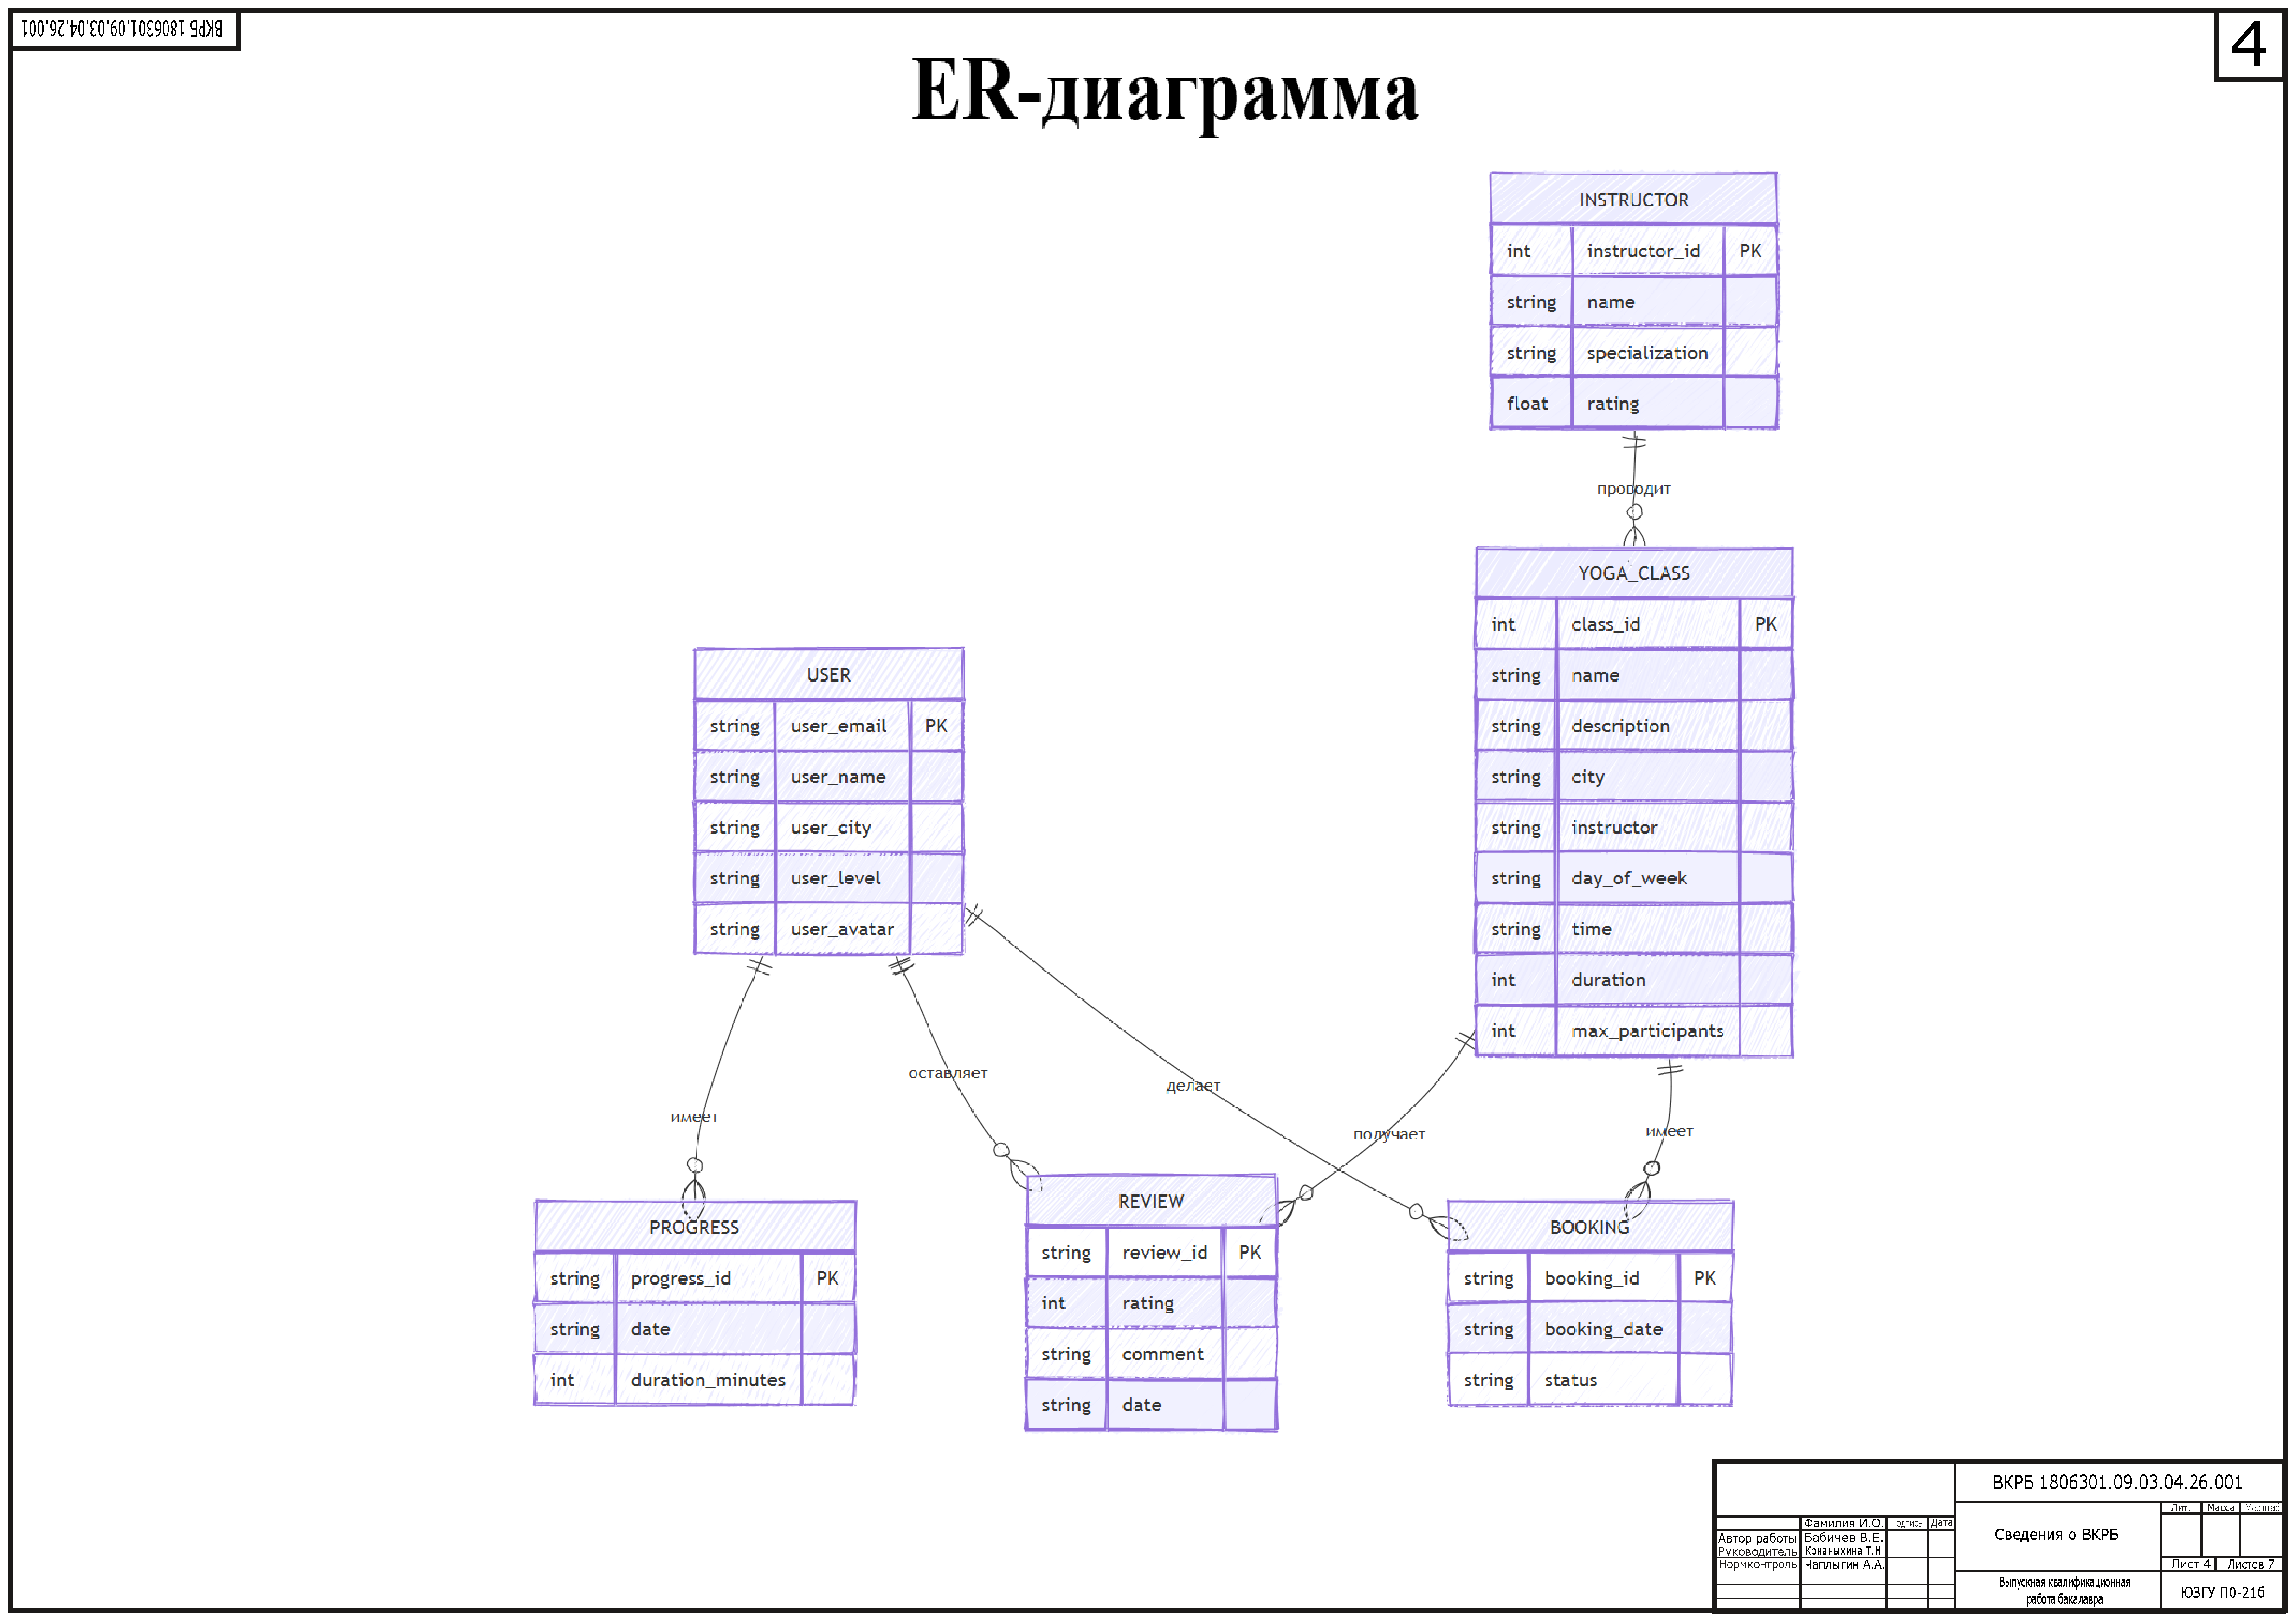
\includegraphics[width=0.82\linewidth]{images/Ramka_VKR4.eps}
		\заголовок{Диаграмма классов}
		\label{pl4:image}      
	\end{плакат}
	
	\begin{плакат}
		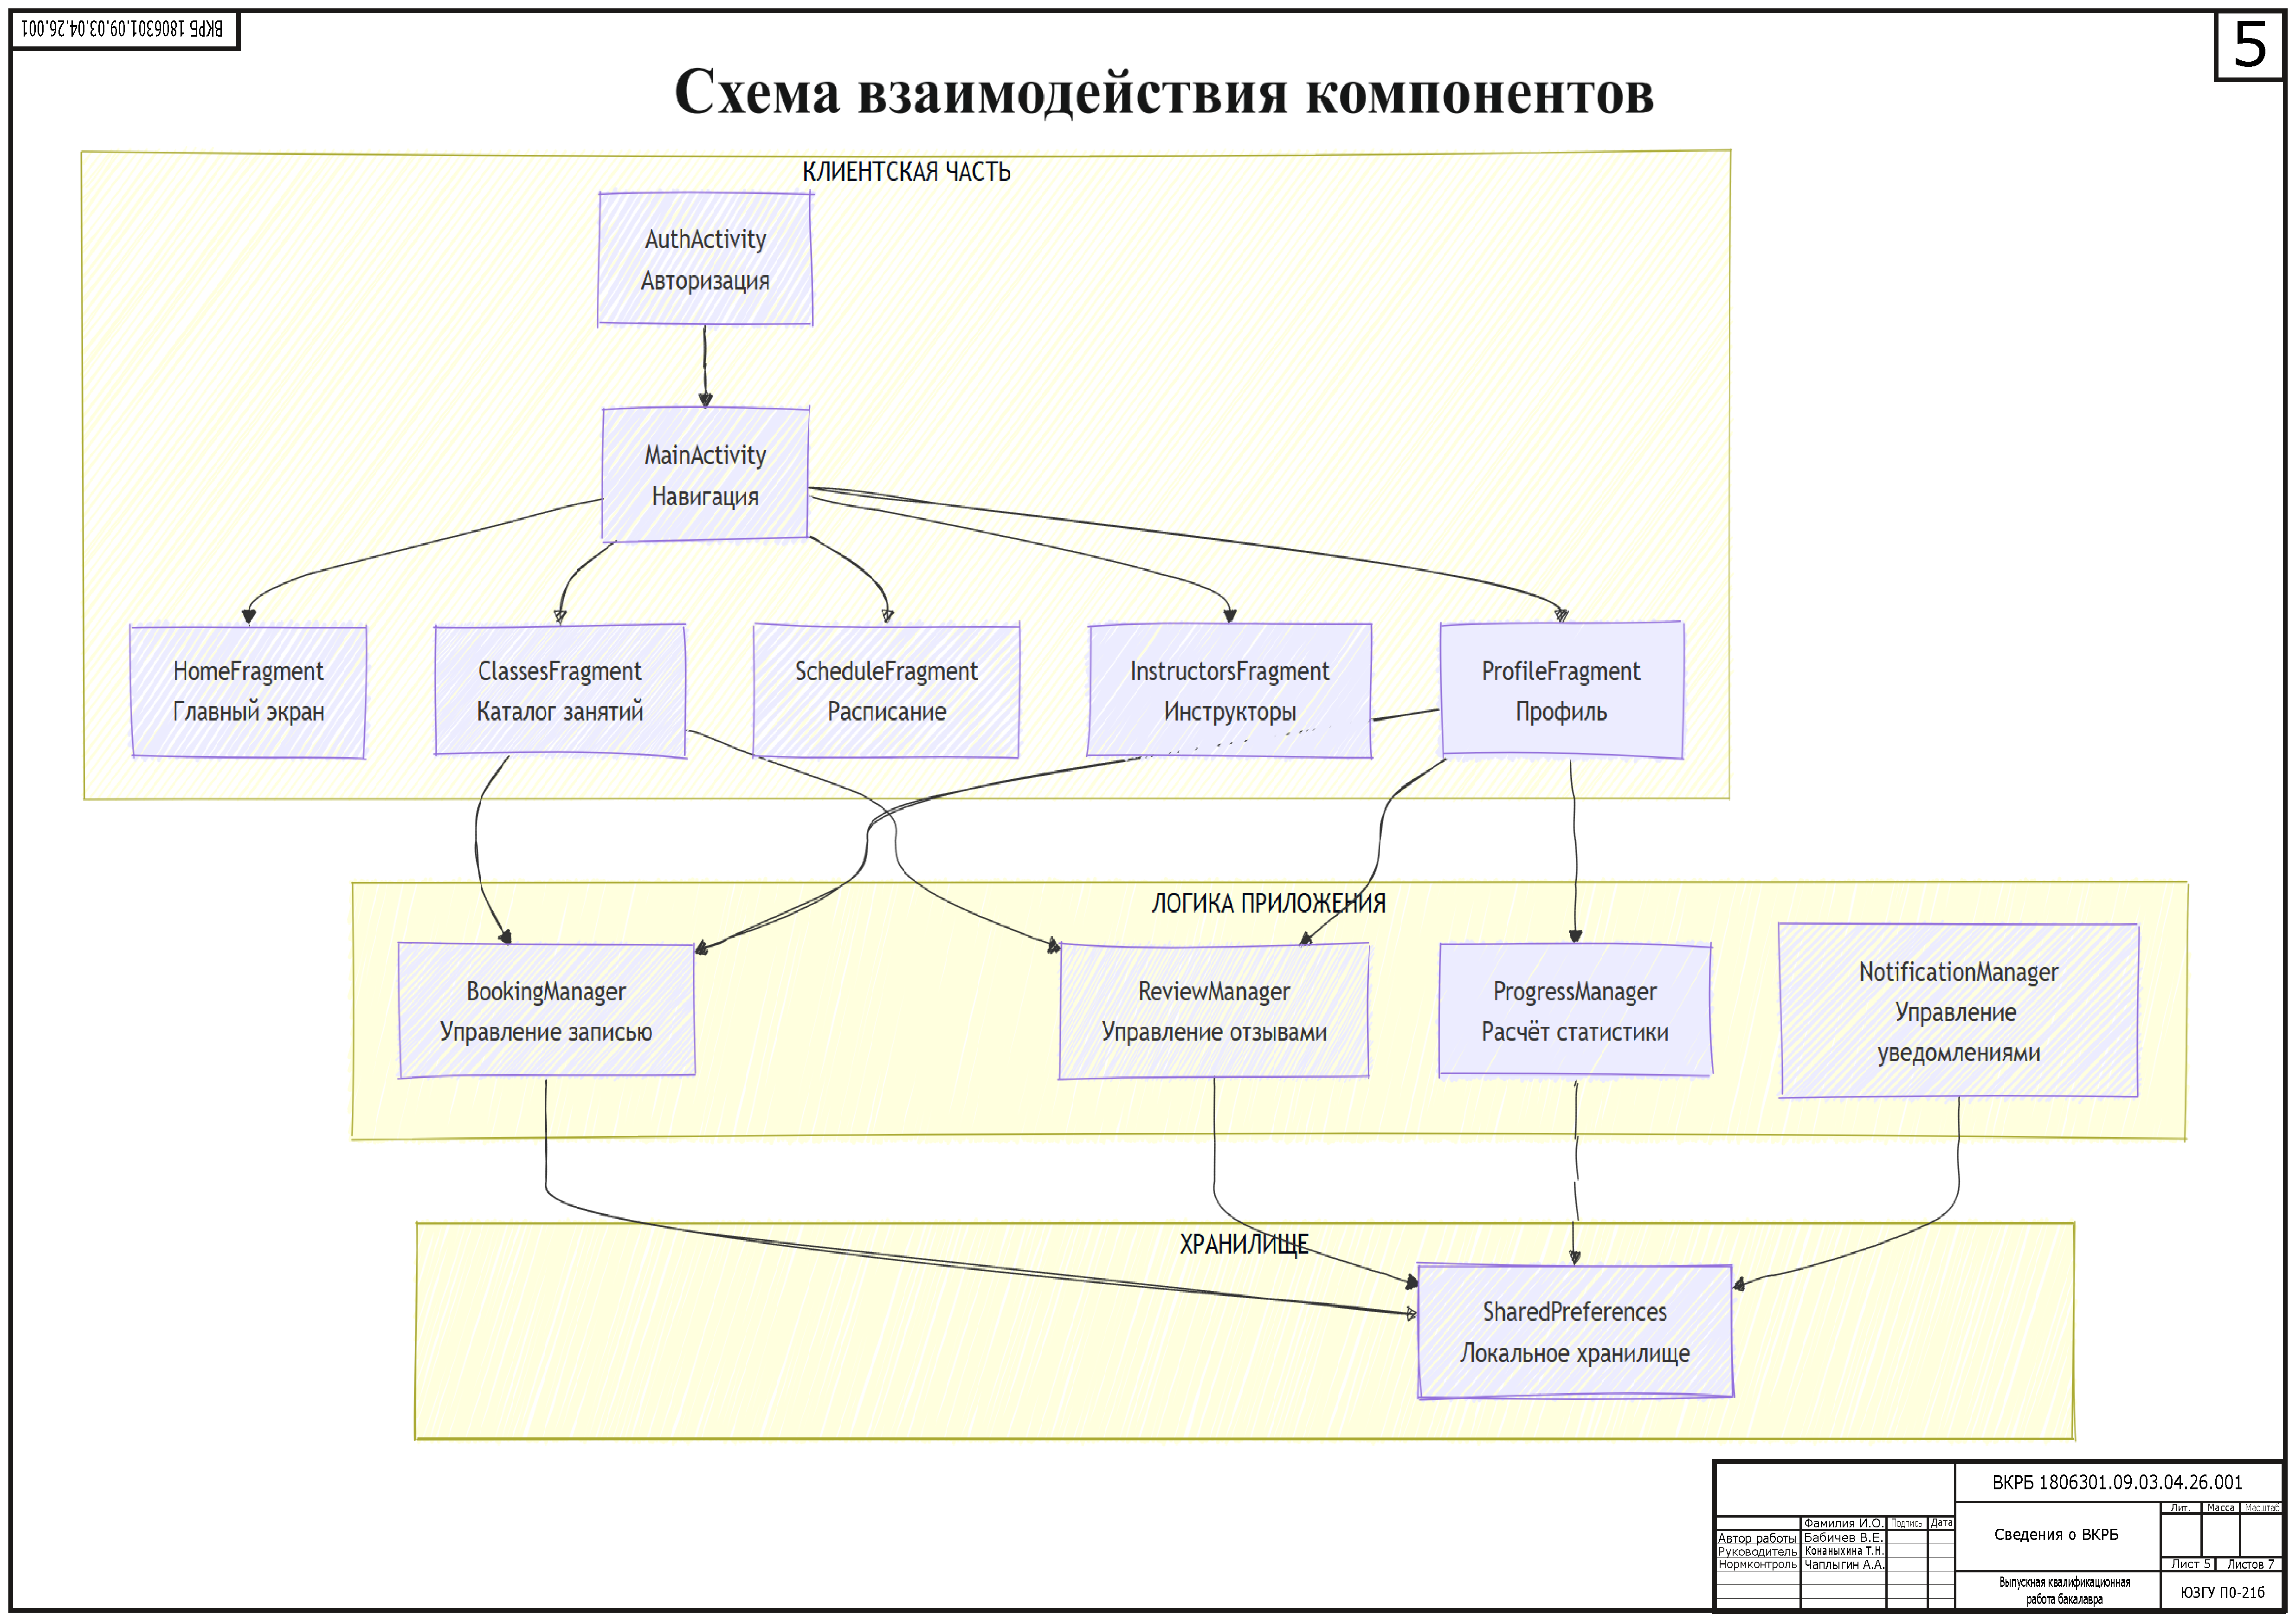
\includegraphics[width=0.82\linewidth]{images/Ramka_VKR5.eps}
		\заголовок{ER-диаграмма сущностей}
		\label{pl5:image}      
	\end{плакат}
	
	\begin{плакат}
		
\includegraphics[width=0.82\linewidth]{images/Ramka_VKR6.eps}
		\заголовок{Диаграмма прецедентов}
		\label{pl6:image}      
	\end{плакат}
	
	\begin{плакат}
		
\includegraphics[width=0.82\linewidth]{images/Ramka_VKR7.eps}
		\заголовок{Заключение}
		\label{pl7:image}      
	\end{плакат}
	
\end{landscape}}\fi
\ifПрактика{}\else{\appendix{Листинги программного кода}

\subsection{Модуль авторизации (AuthActivity.kt)}

\begin{lstlisting}[breaklines=true]
	class AuthActivity : AppCompatActivity() {
		
		private lateinit var binding: ActivityAuthBinding
		
		override fun onCreate(savedInstanceState: Bundle?) {
			super.onCreate(savedInstanceState)
			binding = ActivityAuthBinding.inflate(layoutInflater)
			setContentView(binding.root)
			
			setupClickListeners()
		}
		
		private fun setupClickListeners() {
			binding.btnLogin.setOnClickListener {
				val email = binding.etEmail.text.toString()
				val password = binding.etPassword.text.toString()
				loginUser(email, password)
			}
			
			binding.btnRegister.setOnClickListener {
				val email = binding.etEmail.text.toString()
				val password = binding.etPassword.text.toString()
				val name = binding.etName.text.toString()
				registerUser(email, password, name)
			}
		}
		
		private fun loginUser(email: String, password: String) {
			val prefs = getSharedPreferences("user_prefs", MODE_PRIVATE)
			val savedPassword = prefs.getString("password_$email", null)
			
			if (savedPassword == password) {
				prefs.edit().putBoolean("is_logged_in", true).apply()
				startActivity(Intent(this, MainActivity::class.java))
				finish()
			} else {
				Toast.makeText(
				this, 
				"Неверный email или пароль", 
				Toast.LENGTH_SHORT
				).show()
			}
		}
		
		private fun registerUser(email: String, password: String, name: String) {
			val prefs = getSharedPreferences("user_prefs", MODE_PRIVATE)
			
			if (prefs.contains("password_$email")) {
				Toast.makeText(
				this, 
				"Пользователь уже существует", 
				Toast.LENGTH_SHORT
				).show()
				return
			}
			
			prefs.edit().apply {
				putString("password_$email", password)
				putString("name_$email", name)
				putBoolean("is_logged_in", true)
				apply()
			}
			
			startActivity(Intent(this, MainActivity::class.java))
			finish()
		}
	}
\end{lstlisting}

\subsection{Модуль каталога занятий (ClassesFragment.kt)}

\begin{lstlisting}[breaklines=true]
	class ClassesFragment : Fragment() {
		
		private lateinit var binding: FragmentClassesBinding
		private lateinit var adapter: ClassesAdapter
		
		override fun onCreateView(
		inflater: LayoutInflater,
		container: ViewGroup?,
		savedInstanceState: Bundle?
		): View {
			binding = FragmentClassesBinding.inflate(
			inflater, 
			container, 
			false
			)
			return binding.root
		}
		
		override fun onViewCreated(view: View, savedInstanceState: Bundle?) {
			super.onViewCreated(view, savedInstanceState)
			setupRecyclerView()
			loadClasses()
			setupSpinner()
		}
		
		private fun setupRecyclerView() {
			adapter = ClassesAdapter { classItem ->
				showClassDetails(classItem)
			}
			binding.rvClasses.adapter = adapter
			binding.rvClasses.layoutManager = LinearLayoutManager(context)
		}
		
		private fun loadClasses() {
			val prefs = requireContext().getSharedPreferences(
			"classes_prefs", 
			MODE_PRIVATE
			)
			val classesJson = prefs.getString("classes_list", "[]")
			val gson = Gson()
			val type = object : TypeToken<List<ClassItem>>() {}.type
			val classes: List<ClassItem> = gson.fromJson(classesJson, type)
			adapter.submitList(classes)
		}
		
		private fun setupSpinner() {
			val cities = listOf("Москва", "Санкт-Петербург", "Казань")
			val adapter = ArrayAdapter(
			requireContext(), 
			android.R.layout.simple_spinner_item, 
			cities
			)
			binding.spinnerCity.adapter = adapter
			
			binding.spinnerCity.onItemSelectedListener = object :
			OnItemSelectedListener {
				
				override fun onItemSelected(
				parent: AdapterView<*>,
				view: View?,
				position: Int,
				id: Long
				) {
					val selectedCity = cities[position]
					filterClassesByCity(selectedCity)
				}
				
				override fun onNothingSelected(parent: AdapterView<*>) {}
			}
		}
		
		private fun filterClassesByCity(city: String) {
			val prefs = requireContext().getSharedPreferences(
			"classes_prefs", 
			MODE_PRIVATE
			)
			val classesJson = prefs.getString("classes_list", "[]")
			val gson = Gson()
			val type = object : TypeToken<List<ClassItem>>() {}.type
			val allClasses: List<ClassItem> = gson.fromJson(classesJson, type)
			val filtered = allClasses.filter { it.city == city }
			adapter.submitList(filtered)
		}
		
		private fun showClassDetails(classItem: ClassItem) {
			val intent = Intent(context, ClassDetailActivity::class.java)
			intent.putExtra("class_item", Gson().toJson(classItem))
			startActivity(intent)
		}
	}
\end{lstlisting}

\subsection{Модуль профиля пользователя (ProfileFragment.kt)}

\begin{lstlisting}[breaklines=true]
	class ProfileFragment : Fragment() {
		
		private lateinit var binding: FragmentProfileBinding
		
		override fun onCreateView(
		inflater: LayoutInflater,
		container: ViewGroup?,
		savedInstanceState: Bundle?
		): View {
			binding = FragmentProfileBinding.inflate(
			inflater, 
			container, 
			false
			)
			return binding.root
		}
		
		override fun onViewCreated(view: View, savedInstanceState: Bundle?) {
			super.onViewCreated(view, savedInstanceState)
			loadProfileData()
			setupClickListeners()
		}
		
		private fun loadProfileData() {
			val prefs = requireContext().getSharedPreferences(
			"user_prefs", 
			MODE_PRIVATE
			)
			val email = prefs.getString("user_email", "")
			val name = prefs.getString("user_name", "")
			val city = prefs.getString("user_city", "")
			val level = prefs.getString("user_level", "")
			
			binding.tvEmail.text = email
			binding.tvName.text = name
			binding.tvCity.text = city
			binding.tvLevel.text = level
		}
		
		private fun setupClickListeners() {
			binding.btnEditProfile.setOnClickListener {
				showEditProfileDialog()
			}
			
			binding.btnLogout.setOnClickListener {
				logout()
			}
		}
		
		private fun logout() {
			val prefs = requireContext().getSharedPreferences(
			"user_prefs", 
			MODE_PRIVATE
			)
			prefs.edit().putBoolean("is_logged_in", false).apply()
			startActivity(Intent(context, AuthActivity::class.java))
			requireActivity().finish()
		}
		
		private fun showEditProfileDialog() {
			val dialogView = layoutInflater.inflate(R.layout.dialog_edit_profile, null)
			val dialog = AlertDialog.Builder(requireContext())
			.setTitle("Редактирование профиля")
			.setView(dialogView)
			.setPositiveButton("Сохранить") { _, _ ->
				val newName = dialogView.findViewById<EditText>(R.id.etName).text.toString()
				val newCity = dialogView.findViewById<EditText>(R.id.etCity).text.toString()
				val newLevel = dialogView.findViewById<EditText>(R.id.etLevel).text.toString()
				saveProfileData(newName, newCity, newLevel)
			}
			.setNegativeButton("Отмена", null)
			.create()
			dialog.show()
		}
		
		private fun saveProfileData(name: String, city: String, level: String) {
			val prefs = requireContext().getSharedPreferences("user_prefs", MODE_PRIVATE)
			prefs.edit().apply {
				putString("user_name", name)
				putString("user_city", city)
				putString("user_level", level)
				apply()
			}
			loadProfileData()
			Toast.makeText(context, "Профиль обновлён", Toast.LENGTH_SHORT).show()
		}
	}
\end{lstlisting}

\subsection{Модуль расписания (ScheduleFragment.kt)}

\begin{lstlisting}[breaklines=true]
	class ScheduleFragment : Fragment() {
		
		private lateinit var binding: FragmentScheduleBinding
		private lateinit var adapter: ScheduleAdapter
		private var selectedDate: Calendar = Calendar.getInstance()
		
		override fun onCreateView(
		inflater: LayoutInflater,
		container: ViewGroup?,
		savedInstanceState: Bundle?
		): View {
			binding = FragmentScheduleBinding.inflate(inflater, container, false)
			return binding.root
		}
		
		override fun onViewCreated(view: View, savedInstanceState: Bundle?) {
			super.onViewCreated(view, savedInstanceState)
			setupCalendar()
			setupRecyclerView()
			loadClassesForDate(selectedDate)
		}
		
		private fun setupCalendar() {
			binding.calendarView.setOnDateChangeListener { _, year, month, dayOfMonth ->
				selectedDate.set(year, month, dayOfMonth)
				loadClassesForDate(selectedDate)
			}
		}
		
		private fun setupRecyclerView() {
			adapter = ScheduleAdapter { classItem ->
				showClassDetails(classItem)
			}
			binding.rvSchedule.adapter = adapter
			binding.rvSchedule.layoutManager = LinearLayoutManager(context)
		}
		
		private fun loadClassesForDate(date: Calendar) {
			val prefs = requireContext().getSharedPreferences("classes_prefs", MODE_PRIVATE)
			val classesJson = prefs.getString("classes_list", "[]")
			val gson = Gson()
			val type = object : TypeToken<List<ClassItem>>() {}.type
			val allClasses: List<ClassItem> = gson.fromJson(classesJson, type)
			
			val dayOfWeek = getDayOfWeek(date.get(Calendar.DAY_OF_WEEK))
			val filtered = allClasses.filter { it.dayOfWeek == dayOfWeek }
			adapter.submitList(filtered)
			
			if (filtered.isEmpty()) {
				binding.tvEmptySchedule.visibility = View.VISIBLE
			} else {
				binding.tvEmptySchedule.visibility = View.GONE
			}
		}
		
		private fun getDayOfWeek(calendarDay: Int): String {
			return when (calendarDay) {
				Calendar.MONDAY -> "ПН"
				Calendar.TUESDAY -> "ВТ"
				Calendar.WEDNESDAY -> "СР"
				Calendar.THURSDAY -> "ЧТ"
				Calendar.FRIDAY -> "ПТ"
				Calendar.SATURDAY -> "СБ"
				Calendar.SUNDAY -> "ВС"
				else -> "ПН"
			}
		}
		
		private fun showClassDetails(classItem: ClassItem) {
			val intent = Intent(context, ClassDetailActivity::class.java)
			intent.putExtra("class_item", Gson().toJson(classItem))
			startActivity(intent)
		}
	}
\end{lstlisting}

\subsection{Модуль отзывов и рейтинга (ReviewFragment.kt)}

\begin{lstlisting}[breaklines=true]
	class ReviewFragment : Fragment() {
		
		private lateinit var binding: FragmentReviewBinding
		private var classItem: ClassItem? = null
		private var selectedRating: Float = 0f
		
		override fun onCreateView(
		inflater: LayoutInflater,
		container: ViewGroup?,
		savedInstanceState: Bundle?
		): View {
			binding = FragmentReviewBinding.inflate(inflater, container, false)
			return binding.root
		}
		
		override fun onViewCreated(view: View, savedInstanceState: Bundle?) {
			super.onViewCreated(view, savedInstanceState)
			
			classItem = arguments?.getString("class_item")?.let {
				Gson().fromJson(it, ClassItem::class.java)
			}
			
			setupRatingBar()
			setupClickListeners()
			loadExistingReview()
		}
		
		private fun setupRatingBar() {
			binding.ratingBar.setOnRatingBarChangeListener { _, rating, _ ->
				selectedRating = rating
			}
		}
		
		private fun setupClickListeners() {
			binding.btnSubmit.setOnClickListener {
				val comment = binding.etComment.text.toString()
				if (selectedRating > 0) {
					saveReview(comment, selectedRating)
				} else {
					Toast.makeText(context, "Выберите рейтинг", Toast.LENGTH_SHORT).show()
				}
			}
		}
		
		private fun saveReview(comment: String, rating: Float) {
			val prefs = requireContext().getSharedPreferences("reviews_prefs", MODE_PRIVATE)
			val userPrefs = requireContext().getSharedPreferences("user_prefs", MODE_PRIVATE)
			val userEmail = userPrefs.getString("user_email", "")
			
			val reviewId = "${userEmail}_${classItem?.id}_${System.currentTimeMillis()}"
			val review = Review(
			id = reviewId,
			userEmail = userEmail ?: "",
			classId = classItem?.id ?: 0,
			rating = rating.toInt(),
			comment = comment,
			date = SimpleDateFormat("yyyy-MM-dd", Locale.getDefault()).format(Date())
			)
			
			val gson = Gson()
			val existingReviewsJson = prefs.getString("reviews_list", "[]")
			val type = object : TypeToken<MutableList<Review>>() {}.type
			val reviews: MutableList<Review> = gson.fromJson(existingReviewsJson, type)
			reviews.add(review)
			prefs.edit().putString("reviews_list", gson.toJson(reviews)).apply()
			
			Toast.makeText(context, "Спасибо за отзыв!", Toast.LENGTH_SHORT).show()
			requireActivity().onBackPressedDispatcher.onBackPressed()
		}
		
		private fun loadExistingReview() {
			// Загрузка существующего отзыва для редактирования
		}
	}
\end{lstlisting}

\subsection{Модуль статистики и графиков (ProgressFragment.kt)}

\begin{lstlisting}[breaklines=true]
	class ProgressFragment : Fragment() {
		
		private lateinit var binding: FragmentProgressBinding
		private lateinit var lineChart: LineChart
		
		override fun onCreateView(
		inflater: LayoutInflater,
		container: ViewGroup?,
		savedInstanceState: Bundle?
		): View {
			binding = FragmentProgressBinding.inflate(inflater, container, false)
			return binding.root
		}
		
		override fun onViewCreated(view: View, savedInstanceState: Bundle?) {
			super.onViewCreated(view, savedInstanceState)
			setupChart()
			loadProgressData()
		}
		
		private fun setupChart() {
			lineChart = binding.lineChart
			lineChart.description.isEnabled = false
			lineChart.axisLeft.setDrawGridLines(true)
			lineChart.xAxis.setDrawGridLines(false)
			lineChart.axisRight.isEnabled = false
			lineChart.legend.isEnabled = true
			lineChart.setTouchEnabled(true)
			lineChart.setDragEnabled(true)
			lineChart.setScaleEnabled(true)
		}
		
		private fun loadProgressData() {
			val prefs = requireContext().getSharedPreferences("progress_prefs", MODE_PRIVATE)
			val progressJson = prefs.getString("progress_list", "[]")
			val gson = Gson()
			val type = object : TypeToken<List<ProgressEntry>>() {}.type
			val progressList: List<ProgressEntry> = gson.fromJson(progressJson, type)
			
			updateStats(progressList)
			updateChart(progressList)
		}
		
		private fun updateStats(progressList: List<ProgressEntry>) {
			val totalClasses = progressList.size
			val totalMinutes = progressList.sumOf { it.durationMinutes }
			val uniqueMonths = progressList.map { it.date.substring(0, 7) }.distinct().size
			
			binding.tvTotalClasses.text = totalClasses.toString()
			binding.tvTotalMinutes.text = totalMinutes.toString()
			binding.tvTotalMonths.text = uniqueMonths.toString()
		}
		
		private fun updateChart(progressList: List<ProgressEntry>) {
			val entries = mutableListOf<Entry>()
			val monthMap = progressList.groupBy { it.date.substring(0, 7) }
			.mapValues { it.value.size }
			.toSortedMap()
			
			var index = 0f
			monthMap.forEach { (month, count) ->
				entries.add(Entry(index, count.toFloat()))
				index++
			}
			
			val dataSet = LineDataSet(entries, "Количество занятий")
			dataSet.color = Color.rgb(255, 87, 34)
			dataSet.setCircleColor(Color.rgb(255, 87, 34))
			dataSet.lineWidth = 2f
			dataSet.circleRadius = 4f
			dataSet.setDrawCircleHole(false)
			dataSet.valueTextSize = 10f
			dataSet.setDrawFilled(true)
			dataSet.fillColor = Color.rgb(255, 87, 34)
			dataSet.fillAlpha = 50
			
			val xAxisLabels = monthMap.keys.toList()
			val xAxis = lineChart.xAxis
			xAxis.valueFormatter = IndexAxisValueFormatter(xAxisLabels)
			xAxis.labelRotationAngle = -45f
			xAxis.granularity = 1f
			
			val lineData = LineData(dataSet)
			lineChart.data = lineData
			lineChart.invalidate()
		}
	}
\end{lstlisting}

\subsection{Модуль уведомлений (NotificationHelper.kt)}

\begin{lstlisting}[breaklines=true]
	class NotificationHelper(private val context: Context) {
		
		companion object {
			const val CHANNEL_ID = "yoga_studio_channel"
			const val CHANNEL_NAME = "Йога-студия"
			const val NOTIFICATION_ID_BOOKING = 1001
			const val NOTIFICATION_ID_REMINDER = 1002
		}
		
		fun createNotificationChannel() {
			if (Build.VERSION.SDK_INT >= Build.VERSION_CODES.O) {
				val channel = NotificationChannel(
				CHANNEL_ID,
				CHANNEL_NAME,
				NotificationManager.IMPORTANCE_HIGH
				).apply {
					description = "Уведомления о записи на занятия и напоминания"
					enableLights(true)
					lightColor = Color.RED
					enableVibration(true)
				}
				
				val notificationManager = context.getSystemService(Context.NOTIFICATION_SERVICE) as NotificationManager
				notificationManager.createNotificationChannel(channel)
			}
		}
		
		fun sendBookingConfirmation(className: String, date: String, time: String) {
			val notification = NotificationCompat.Builder(context, CHANNEL_ID)
			.setSmallIcon(android.R.drawable.ic_dialog_info)
			.setContentTitle("Запись подтверждена")
			.setContentText("Вы записаны на занятие \"$className\" $date в $time")
			.setPriority(NotificationCompat.PRIORITY_HIGH)
			.setAutoCancel(true)
			.build()
			
			val notificationManager = NotificationManagerCompat.from(context)
			notificationManager.notify(NOTIFICATION_ID_BOOKING, notification)
		}
		
		fun sendReminder(className: String, time: String) {
			val notification = NotificationCompat.Builder(context, CHANNEL_ID)
			.setSmallIcon(android.R.drawable.ic_dialog_info)
			.setContentTitle("Напоминание о занятии")
			.setContentText("Занятие \"$className\" начнётся через 1 час в $time")
			.setPriority(NotificationCompat.PRIORITY_HIGH)
			.setAutoCancel(true)
			.build()
			
			val notificationManager = NotificationManagerCompat.from(context)
			notificationManager.notify(NOTIFICATION_ID_REMINDER, notification)
		}
		
		fun scheduleReminder(className: String, time: String, timestamp: Long) {
			val alarmManager = context.getSystemService(Context.ALARM_SERVICE) as AlarmManager
			val intent = Intent(context, ReminderReceiver::class.java).apply {
				putExtra("class_name", className)
				putExtra("class_time", time)
			}
			
			val pendingIntent = PendingIntent.getBroadcast(
			context,
			NOTIFICATION_ID_REMINDER,
			intent,
			PendingIntent.FLAG_UPDATE_CURRENT or PendingIntent.FLAG_IMMUTABLE
			)
			
			val reminderTime = timestamp - 60 * 60 * 1000 // за 1 час до занятия
			
			if (Build.VERSION.SDK_INT >= Build.VERSION_CODES.M) {
				alarmManager.setExactAndAllowWhileIdle(
				AlarmManager.RTC_WAKEUP,
				reminderTime,
				pendingIntent
				)
			} else {
				alarmManager.setExact(AlarmManager.RTC_WAKEUP, reminderTime, pendingIntent)
			}
		}
	}
	
	class ReminderReceiver : BroadcastReceiver() {
		override fun onReceive(context: Context, intent: Intent) {
			val className = intent.getStringExtra("class_name") ?: ""
			val classTime = intent.getStringExtra("class_time") ?: ""
			
			val notificationHelper = NotificationHelper(context)
			notificationHelper.sendReminder(className, classTime)
		}
	}
\end{lstlisting}

\subsection{Модели данных (Data Models.kt)}

\begin{lstlisting}[breaklines=true]
	data class User(
	val email: String,
	val name: String,
	val city: String,
	val level: String,
	val avatarUri: String? = null
	)
	
	data class ClassItem(
	val id: Int,
	val name: String,
	val description: String,
	val city: String,
	val instructor: String,
	val dayOfWeek: String,
	val time: String,
	val duration: Int,
	val maxParticipants: Int,
	val currentParticipants: Int,
	val price: Double = 0.0
	)
	
	data class Instructor(
	val id: Int,
	val name: String,
	val specialization: String,
	val city: String,
	val rating: Float,
	val bio: String? = null,
	val photoUrl: String? = null
	)
	
	data class Booking(
	val id: String,
	val userEmail: String,
	val classId: Int,
	val bookingDate: String,
	val status: String // "active", "cancelled", "completed"
	)
	
	data class Review(
	val id: String,
	val userEmail: String,
	val classId: Int,
	val rating: Int,
	val comment: String,
	val date: String
	)
	
	data class ProgressEntry(
	val id: String,
	val userEmail: String,
	val date: String,
	val durationMinutes: Int,
	val calories: Int = 0,
	val classType: String? = null
	)
	
	data class NotificationData(
	val id: String,
	val userEmail: String,
	val title: String,
	val message: String,
	val timestamp: Long,
	val isRead: Boolean = false
	)
\end{lstlisting}

\subsection{SharedPreferences Manager (PrefsManager.kt)}

\begin{lstlisting}[breaklines=true]
	class PrefsManager(private val context: Context) {
		
		private val prefs = context.getSharedPreferences("app_prefs", Context.MODE_PRIVATE)
		private val gson = Gson()
		
		fun saveUser(user: User) {
			prefs.edit().putString("user_${user.email}", gson.toJson(user)).apply()
			prefs.edit().putString("current_user", user.email).apply()
		}
		
		fun getCurrentUser(): User? {
			val email = prefs.getString("current_user", null) ?: return null
			val userJson = prefs.getString("user_$email", null) ?: return null
			return gson.fromJson(userJson, User::class.java)
		}
		
		fun saveBookings(bookings: List<Booking>) {
			prefs.edit().putString("bookings", gson.toJson(bookings)).apply()
		}
		
		fun getBookings(): List<Booking> {
			val json = prefs.getString("bookings", "[]")
			val type = object : TypeToken<List<Booking>>() {}.type
			return gson.fromJson(json, type)
		}
		
		fun saveClasses(classes: List<ClassItem>) {
			prefs.edit().putString("classes", gson.toJson(classes)).apply()
		}
		
		fun getClasses(): List<ClassItem> {
			val json = prefs.getString("classes", "[]")
			val type = object : TypeToken<List<ClassItem>>() {}.type
			return gson.fromJson(json, type)
		}
		
		fun saveReviews(reviews: List<Review>) {
			prefs.edit().putString("reviews", gson.toJson(reviews)).apply()
		}
		
		fun getReviews(): List<Review> {
			val json = prefs.getString("reviews", "[]")
			val type = object : TypeToken<List<Review>>() {}.type
			return gson.fromJson(json, type)
		}
		
		fun isLoggedIn(): Boolean {
			return prefs.getString("current_user", null) != null
		}
		
		fun logout() {
			prefs.edit().remove("current_user").apply()
		}
		
		fun clearAll() {
			prefs.edit().clear().apply()
		}
	}
\end{lstlisting}}\fi
\end{document}
